% presentacion.tex — presentación final del proyecto PI3 (25 de septiembre de 2026).
%
% Ningún número del proyecto está tecleado aquí: todos entran por los fragmentos
% que genera experiments/make_presentation.py bajo
% results/figures/presentation/fragments/, y las figuras de datos salen del mismo
% script. Para regenerar todo, ver presentation/README.md.
%
% Compilación (dos pasadas cada una, desde presentation/):
%   lualatex presentacion.tex                                   -> presentacion.pdf
%   lualatex -jobname=presentacion_notas "\def\shownotes{1}% presentacion.tex — presentación final del proyecto PI3 (25 de septiembre de 2026).
%
% Ningún número del proyecto está tecleado aquí: todos entran por los fragmentos
% que genera experiments/make_presentation.py bajo
% results/figures/presentation/fragments/, y las figuras de datos salen del mismo
% script. Para regenerar todo, ver presentation/README.md.
%
% Compilación (dos pasadas cada una, desde presentation/):
%   lualatex presentacion.tex                                   -> presentacion.pdf
%   lualatex -jobname=presentacion_notas "\def\shownotes{1}% presentacion.tex — presentación final del proyecto PI3 (25 de septiembre de 2026).
%
% Ningún número del proyecto está tecleado aquí: todos entran por los fragmentos
% que genera experiments/make_presentation.py bajo
% results/figures/presentation/fragments/, y las figuras de datos salen del mismo
% script. Para regenerar todo, ver presentation/README.md.
%
% Compilación (dos pasadas cada una, desde presentation/):
%   lualatex presentacion.tex                                   -> presentacion.pdf
%   lualatex -jobname=presentacion_notas "\def\shownotes{1}% presentacion.tex — presentación final del proyecto PI3 (25 de septiembre de 2026).
%
% Ningún número del proyecto está tecleado aquí: todos entran por los fragmentos
% que genera experiments/make_presentation.py bajo
% results/figures/presentation/fragments/, y las figuras de datos salen del mismo
% script. Para regenerar todo, ver presentation/README.md.
%
% Compilación (dos pasadas cada una, desde presentation/):
%   lualatex presentacion.tex                                   -> presentacion.pdf
%   lualatex -jobname=presentacion_notas "\def\shownotes{1}\input{presentacion.tex}"
%                                                               -> presentacion_notas.pdf
\documentclass[aspectratio=169,11pt]{beamer}

\usetheme[numbering=fraction,progressbar=none,block=fill,background=light]{metropolis}
\usepackage[spanish,es-noshorthands,es-nodecimaldot]{babel}
\usepackage{amsmath,amssymb}
\usepackage{booktabs}
\usepackage{array}
\usepackage{tikz}
\usetikzlibrary{arrows.meta,positioning,calc,patterns,decorations.pathreplacing,shapes.geometric}
\usepackage{pgfpages}
\usepackage{appendixnumberbeamer}

% notas del orador: activadas con \def\shownotes{1} antes de \input
\ifdefined\shownotes
  \setbeameroption{show notes on second screen=right}
  \setbeamertemplate{note page}[plain]
  \setbeamerfont{note page}{size=\scriptsize}
\fi

% ---------------------------------------------------------------- colores
% Los tres órdenes llevan el mismo color en toda la presentación, y son los mismos
% tres valores hexadecimales que experiments/make_presentation.py usa en las
% figuras. Ninguno se lee como bueno o malo. La intersección se raya, nunca lleva
% un cuarto color.
\definecolor{philu}{HTML}{2A6FB0}
\definecolor{phils}{HTML}{C98A2B}
\definecolor{phicw}{HTML}{7A4FA3}
\definecolor{coefcol}{HTML}{B03A2E}
\definecolor{gris}{HTML}{6A6A6A}
\definecolor{grisclaro}{HTML}{DDDDDD}
\setbeamercolor{alerted text}{fg=coefcol}
\setbeamerfont{title}{size=\Large}

\newcommand{\plu}{\textcolor{philu}{$\phi_{lu}$}}
\newcommand{\pls}{\textcolor{phils}{$\phi_{ls}$}}
\newcommand{\pcw}{\textcolor{phicw}{$\phi_{cw}$}}
\newcommand{\Xlu}{\textcolor{philu}{$X_{lu}$}}
\newcommand{\Xls}{\textcolor{phils}{$X_{ls}$}}
\newcommand{\Xcw}{\textcolor{phicw}{$X_{cw}$}}
\newcommand{\coef}[1]{\textcolor{coefcol}{\boldsymbol{#1}}}
\newcommand{\marca}[1]{\textcolor{coefcol}{\boldsymbol{#1}}}
\newcommand{\cita}[1]{\textcolor{gris}{\small #1}}
\newcommand{\refuno}{[1] Costa, Osuna-Gómez y Chalco-Cano (2024)}
\newcommand{\refdieciseis}{[16] Mondal, Ghosh y Kim (2026)}

% ---------------------------------------------------------------- números generados
\graphicspath{{../results/figures/presentation/}}
\input{../results/figures/presentation/fragments/numbers.tex}
\input{../results/figures/presentation/fragments/notas.tex}

\title{Técnicas de Optimización Intervalar basadas en Inteligencia Computacional}
\subtitle{¿Cuánto cambia la respuesta cuando lo único que cambia es el orden?}
\author{Francisco Rodríguez-Carretero Roldán}
\institute{Tutores: Antonio Beato Moreno y Rafaela Osuna Gómez · Universidad de Sevilla}
\date{25 de septiembre de 2026 · Proyecto PI3, julio--septiembre 2026}

\begin{document}

% ================================================================ portada
\begin{frame}[plain]
  \vspace{-6mm}\titlepage
\end{frame}

% ================================================================ BLOQUE A
% ---------------------------------------------------------------- 1
\begin{frame}{Optimizar con varios objetivos: no hay un ganador, hay un conjunto}
  \begin{columns}[T]
    \begin{column}{0.52\textwidth}
      \centering
      \begin{tikzpicture}[scale=0.55]
        \draw[-{Stealth}] (0,0) -- (10.5,0) node[below left] {coste};
        \draw[-{Stealth}] (0,0) -- (0,9.5) node[below right,rotate=0] {riesgo};
        % dominados
        \foreach \x/\y in {3/7, 5/6, 6/4.5, 8/4, 4/6.5, 7/3.5, 9/5, 2.5/8.5, 5.5/8, 8.5/6.5, 3.5/5.5, 6.5/6}
          \fill[gris!60] (\x,\y) circle (0.14);
        % no dominados
        \draw[dashed,gris] plot[smooth] coordinates {(1,8) (2,5.5) (3.5,4) (5,3) (7,2.2) (9,1.8)};
        \foreach \x/\y in {1/8, 2/5.5, 3.5/4, 5/3, 7/2.2, 9/1.8}
          \fill[philu] (\x,\y) circle (0.2);
        \node[philu,align=left,font=\small] at (7.6,7.8) {conjunto eficiente\\(frente de Pareto)};
        \node[gris,font=\small] at (6.2,1.2) {dominados};
      \end{tikzpicture}
    \end{column}
    \begin{column}{0.46\textwidth}
      Bajar el coste sube el riesgo: no hay una solución única, existe un conjunto
      de soluciones eficientes.
      \begin{block}{Dominancia}
        $A$ domina a $B$ si $A$ es igual o mejor que $B$ en \textbf{todos} los
        objetivos y estrictamente mejor en \textbf{al menos uno}.
      \end{block}
      \vspace{2mm}
      Una solución es \textbf{eficiente} si nadie la domina.\\[2mm]
    \end{column}
  \end{columns}
  \NotaI
\end{frame}

% ---------------------------------------------------------------- 2
\begin{frame}{Bajo incertidumbre, los intervalos no siempre se ordenan intuitivamente}
  \centering
  \begin{tikzpicture}[scale=0.66]
    % el intervalo [38, 45]
    \begin{scope}
      \draw[thick] (0,0) -- (7,0);
      \draw[very thick,philu] (1,0) -- (6,0);
      \draw[very thick,philu] (1,-0.15) -- (1,0.15) node[above] {$38$};
      \draw[very thick,philu] (6,-0.15) -- (6,0.15) node[above] {$45$};
      \fill[philu] (3.5,0) circle (0.07) node[above,text=black] {centro $41.5$};
      \draw[decorate,decoration={brace,mirror,amplitude=4pt}] (1,-0.3) -- (3.5,-0.3)
        node[midway,below=4pt,font=\small,text=black] {semianchura $3.5$};
      \draw[decorate,decoration={brace,mirror,amplitude=4pt}] (1,-1.1) -- (6,-1.1)
        node[midway,below=4pt,font=\small,text=black] {anchura $7$};
      \node[right,font=\small,gris,align=left,text width=4.8cm] at (7.6,0.2) {``el coste no es $40$, es $[38, 45]$''};
    \end{scope}
    % A = [1.5, 5], B = [3, 7.5]
    \begin{scope}[yshift=-4.6cm]
      \draw[-{Stealth}] (0,0) -- (10,0) node[right] {$\mathbb{R}$};
      \foreach \x in {0,1,...,9} \draw (\x,-0.08) -- (\x,0.08) node[below=2pt,font=\scriptsize] {\x};
      \draw[very thick,philu] (1.5,0.5) -- (5,0.5) node[midway,above,font=\small] {$A = [1.5, 5]$};
      \draw[very thick,phicw] (3,1.5) -- (7.5,1.5) node[midway,above,font=\small] {$B = [3, 7.5]$};
      \node[right,font=\small,align=left,text width=4.8cm] at (10.6,0.9) {$A$ empieza y acaba antes:\\ aquí $A$ parece menor.};
    \end{scope}
    \begin{scope}[yshift=-8.2cm]
      \draw[-{Stealth}] (0,0) -- (10,0) node[right] {$\mathbb{R}$};
      \foreach \x in {0,1,...,9} \draw (\x,-0.08) -- (\x,0.08);
      \draw[very thick,philu] (1,0.5) -- (10,0.5) node[midway,above,font=\small] {$A = [1, 10]$};
      \draw[very thick,phicw] (4,1.5) -- (5,1.5) node[midway,above,font=\small] {$B = [4, 5]$};
      \node[right,font=\small,align=left,text width=4.8cm] at (10.6,0.9) {\textbf{¿Cuál es menor?}\\ No hay respuesta.};
    \end{scope}
  \end{tikzpicture}
  \NotaII
\end{frame}

% ---------------------------------------------------------------- 3
\begin{frame}{Una familia entera de órdenes, con un parámetro que dice cuál usas: $\phi$}
  \begin{columns}[c,onlytextwidth]
    \begin{column}{0.27\textwidth}
      \centering
      \begin{tikzpicture}[node distance=3.5mm,every node/.style={font=\small}]
        \node[draw,rounded corners,minimum height=7mm] (in) {$[\,l,\,u\,]$};
        \node[draw,rounded corners,fill=grisclaro,minimum height=7mm,right=of in] (phi) {$\phi$};
        \node[draw,rounded corners,minimum height=7mm,right=of phi] (out) {$(a,\,b)$};
        \draw[-{Stealth}] (in) -- (phi);
        \draw[-{Stealth}] (phi) -- (out);
      \end{tikzpicture}\\[1mm]
      {\small\color{gris} dos reales sí se comparan}
    \end{column}
    \begin{column}{0.71\textwidth}
      \footnotesize\setlength{\tabcolsep}{4pt}
      \begin{tabular}{@{}lll@{}}
        \toprule
        orden & fórmula & qué mira \\
        \midrule
        \plu\ (Ejemplo 2.2) & $[l,u]\mapsto(l,\;u)$ & inferior y superior \\
        \pls\ (Ejemplo 2.3) & $[l,u]\mapsto(l,\;u-l)$ & inferior y \textbf{anchura} \\
        \pcw\ (Ejemplo 2.4) & $[l,u]\mapsto\bigl(\tfrac{l+u}{2},\;\tfrac{u-l}{2}\bigr)$ & centro y \textbf{semianchura} \\
        \bottomrule
      \end{tabular}
    \end{column}
  \end{columns}
  \vspace{4mm}
  \begin{columns}[T]
    \begin{column}{0.48\textwidth}
      \begin{block}{La analogía}
        $\phi$ es la función \texttt{key} de un \texttt{sort}: cambias la
        \texttt{key}, cambia el orden.
      \end{block}
    \end{column}
    \begin{column}{0.48\textwidth}
      \begin{block}{La regla}
        $m$ objetivos intervalares $\to$ $2m$ objetivos reales, y un problema
        real ya se sabe resolver.
      \end{block}
    \end{column}
  \end{columns}
  \vspace{2mm}
  \cita{Ejemplos 2.2, 2.3 y 2.4 de \refuno. Los tres son válidos}
  \NotaIII
\end{frame}

% ---------------------------------------------------------------- 4
\begin{frame}{}
  \vspace{8mm}
  \begin{center}
    {\LARGE\bfseries Si cambio el orden y no cambio nada más,\\[3mm]
     ¿cambia la respuesta? ¿Y cuánto?}
  \end{center}
\end{frame}

% ---------------------------------------------------------------- 5
\begin{frame}{Lo primero que probé fue lo obvio, y no medía nada}
  \centering
  \begin{tikzpicture}[scale=0.82,font=\scriptsize]
    \begin{scope}
      \draw[-{Stealth},gris] (0,-0.4) -- (4.4,-0.4);
      \fill[gris!25] plot[smooth,domain=0.3:4.1] ({\x},{1.5-0.35*\x+0.09*\x*\x+0.45})
        -- plot[smooth,domain=4.1:0.3] ({\x},{1.5-0.35*\x+0.09*\x*\x-0.45}) -- cycle;
      \draw[very thick,philu] plot[smooth,domain=0.3:4.1] ({\x},{1.5-0.35*\x+0.09*\x*\x});
      \draw[<->,coefcol,thick] (3.1,{1.5-0.35*3.1+0.09*3.1*3.1-0.45}) -- (3.1,{1.5-0.35*3.1+0.09*3.1*3.1+0.45})
        node[midway,right=1.2mm,coefcol] {$2\varepsilon$};
      \node[gris,font=\scriptsize,align=center] at (2.2,-1.25) {un margen de error \textbf{siempre igual}};
    \end{scope}
    \begin{scope}[xshift=5.6cm,yshift=1.3cm,font=\small]
      \node[philu] at (0,0.8) {\plu};
      \node[phils] at (0,0) {\pls};
      \node[phicw] at (0,-0.8) {\pcw};
      \node[anchor=west] at (0.4,0.8) {$(f-\varepsilon,\; f+\varepsilon)$};
      \node[anchor=west] at (0.4,0) {$(f-\varepsilon,\; \coef{2\varepsilon})$};
      \node[anchor=west] at (0.4,-0.8) {$(f,\; \coef{\varepsilon})$};
      \node[coefcol,font=\scriptsize,align=center] at (1.6,-1.6) {nunca cambian};
    \end{scope}
    \begin{scope}[xshift=11.2cm,yshift=1.3cm,font=\scriptsize]
      \draw[very thick,phils,fill=phils!12] (0,0) circle (1.25);
      \draw[very thick,philu,dashed] (0,0) circle (1.25);
      \draw[very thick,phicw,dotted] (0,0) circle (1.25);
      \node[align=center] at (0,0) {los tres dan\\la misma\\respuesta};
    \end{scope}
    \draw[-{Stealth},gris,thick] (9.3,1.3) -- (9.8,1.3);
  \end{tikzpicture}

  \vspace{1mm}
  \begin{minipage}{0.84\textwidth}
    \begin{block}{La regla que saqué de aquí}
      La incertidumbre tiene que depender de algo que el valor central no
      controle. Si el ancho se puede calcular a partir del centro, los tres
      órdenes se vuelven el mismo.
    \end{block}
  \end{minipage}
  \NotaV
\end{frame}

% ---------------------------------------------------------------- 6
\begin{frame}{El problema p1, sin incertidumbre todavía: acercarse a dos sitios a la vez}
  \centering
  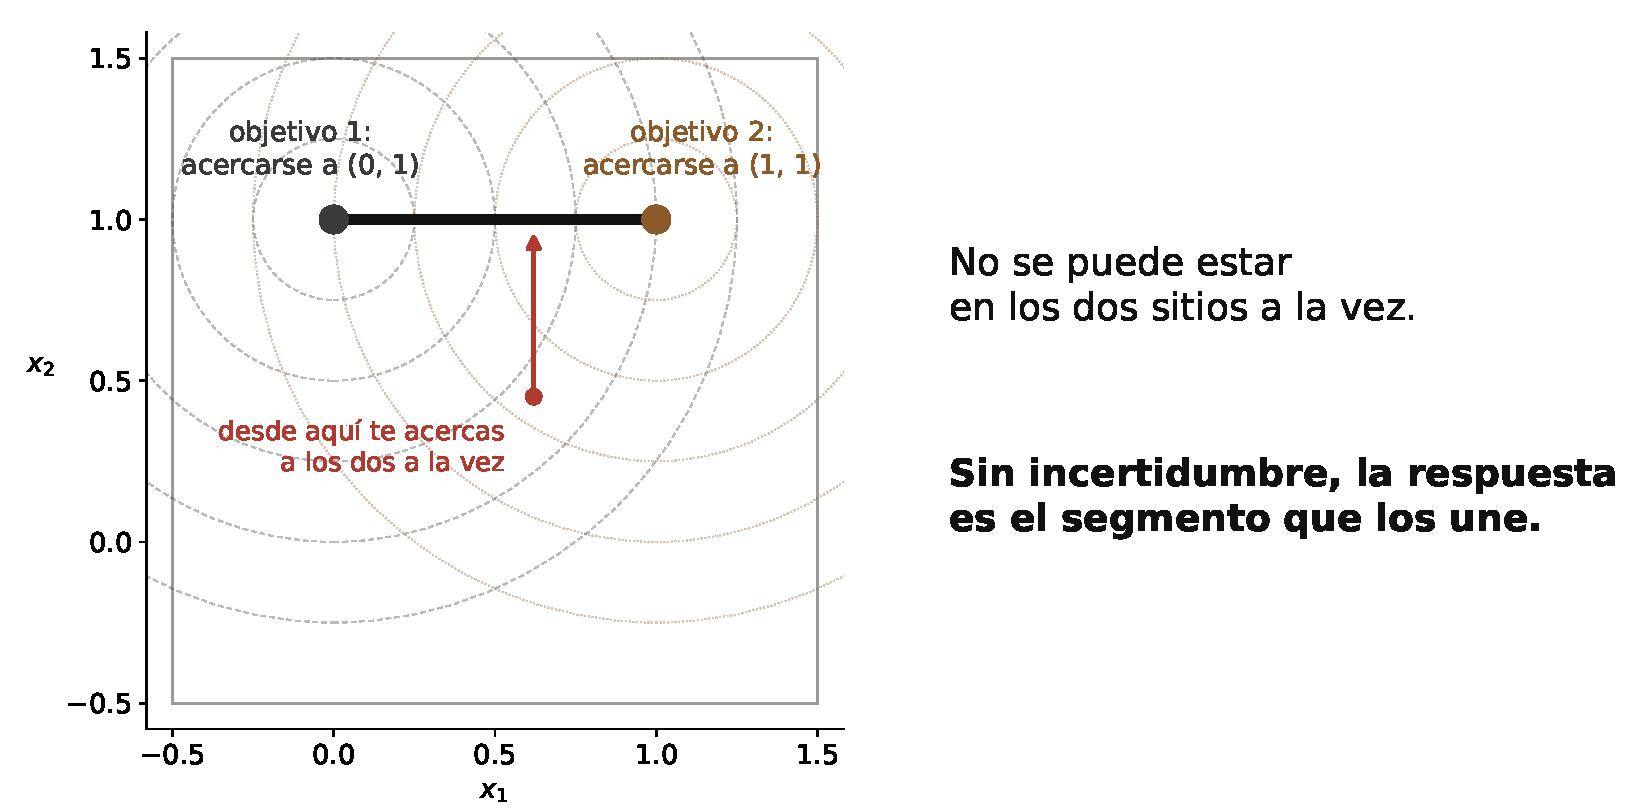
\includegraphics[width=0.99\textwidth,height=0.70\textheight,keepaspectratio]{p1_crisp.pdf}

  \vspace{-2mm}
  {\footnotesize Dos variables, un problema que se puede resolver a mano.}
  \NotaVI
\end{frame}

% ---------------------------------------------------------------- 7
\begin{frame}{p1, tres órdenes, tres respuestas distintas}
  \centering
  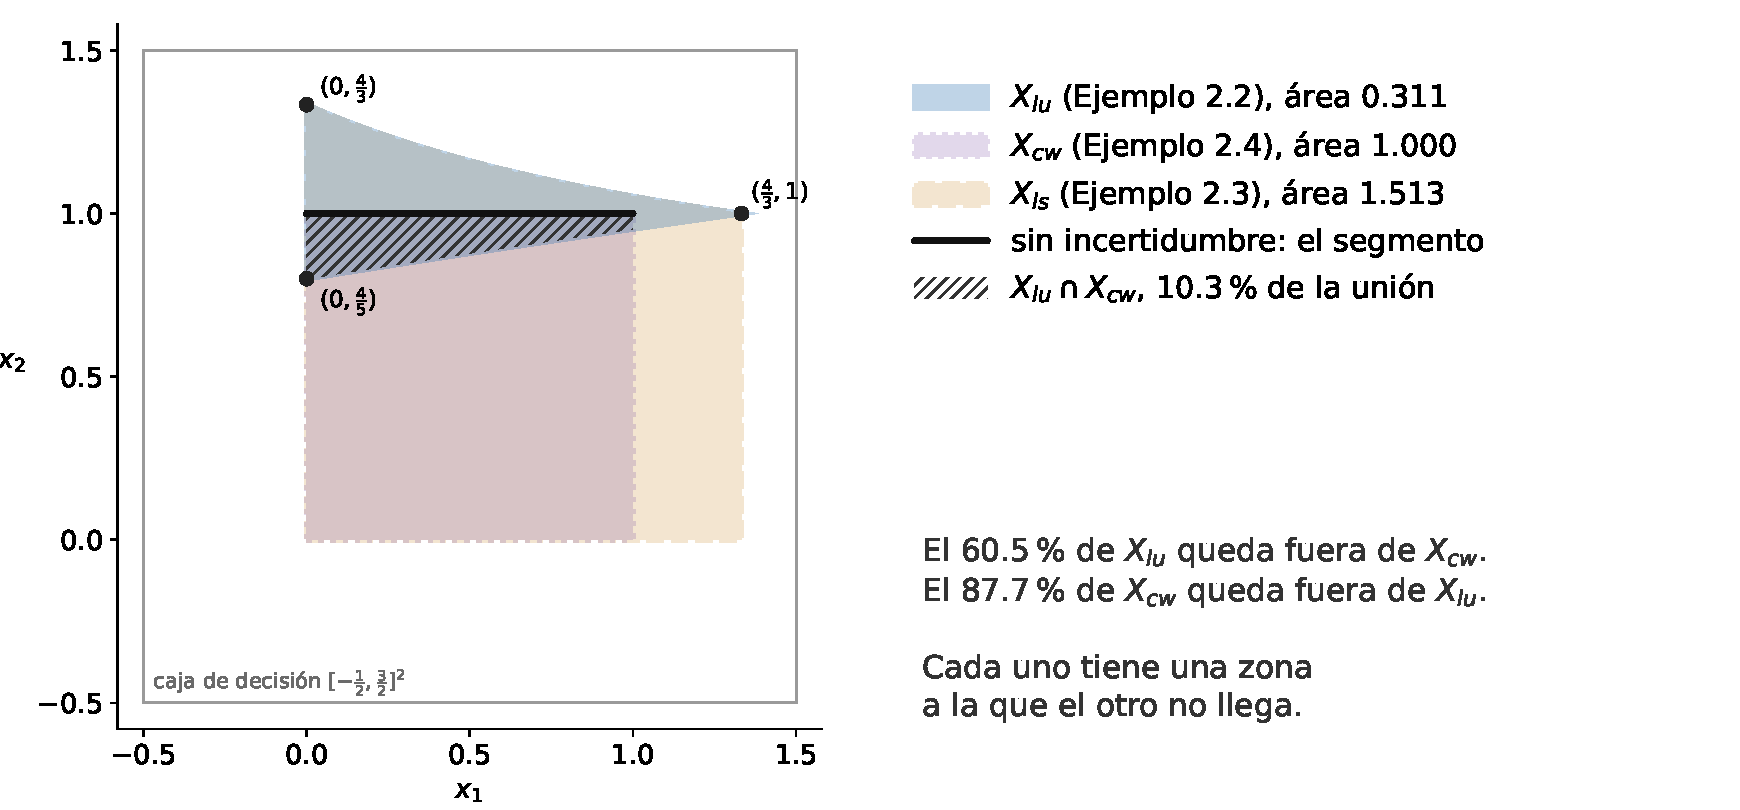
\includegraphics[width=0.98\textwidth,height=0.70\textheight,keepaspectratio]{p1_regiones.pdf}

  \vspace{-2mm}
  {\footnotesize De todo lo que podrían tener en común, sólo comparten el
  \textbf{\pUnionShare\,\%}. \cita{Y esto no lo ha calculado un ordenador: son las tres fórmulas dibujadas.}}
  \NotaVII
\end{frame}

% ---------------------------------------------------------------- 8
\begin{frame}{Y sé cuánto se equivoca lo que uso para medir}
  \centering
  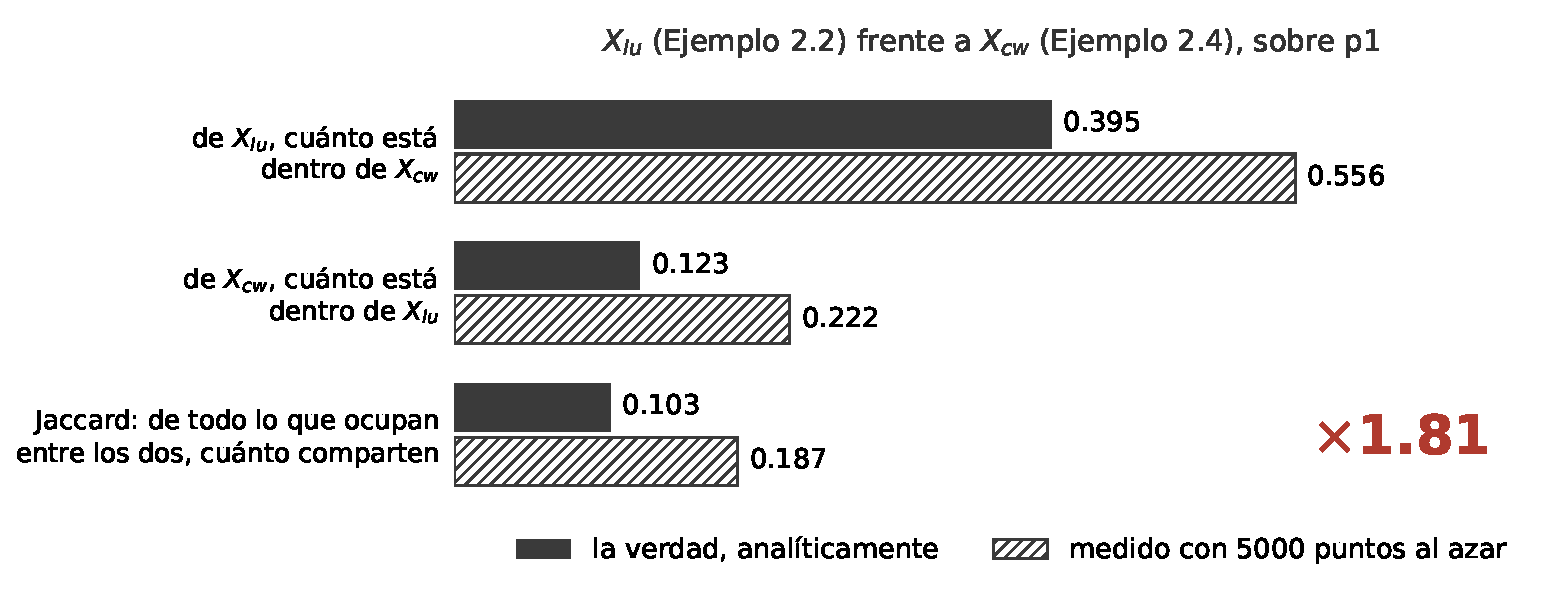
\includegraphics[width=0.97\textwidth,height=0.68\textheight,keepaspectratio]{instrumento.pdf}

  \vspace{-1mm}
  {\small Siempre en la misma dirección: al medir con puntos al azar, los dos
  órdenes salen \textbf{más parecidos de lo que son}.}
  \NotaVIII
\end{frame}

% ---------------------------------------------------------------- 9
\begin{frame}{Y ahora, p2, problemas de referencia del campo}
  \begin{columns}[T,onlytextwidth]
    \begin{column}{0.49\textwidth}
      \centering
      {\large\textbf{\ZdtName}} \quad \cita{\ZdtSize}\\[1mm]
      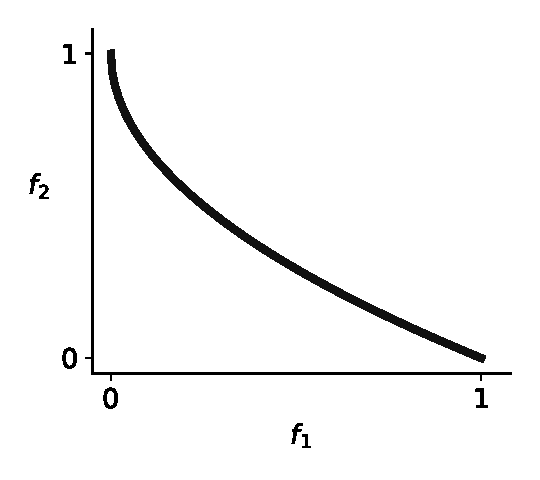
\includegraphics[height=0.33\textheight]{zdt1_frente.pdf}\\[-2mm]
      {\scriptsize $\ZdtF$\\[1mm] $\ZdtG$\\[0.5mm] \phantom{$\ZdtG$}}
    \end{column}
    \begin{column}{0.49\textwidth}
      \centering
      {\large\textbf{\DtlzName}} \quad \cita{\DtlzSize}\\[1mm]
      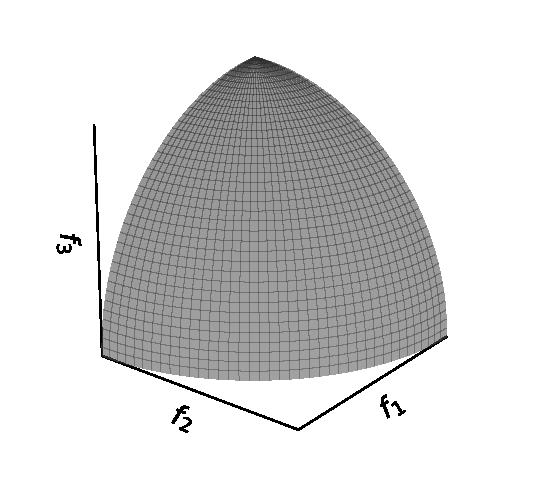
\includegraphics[height=0.33\textheight]{dtlz2_frente.pdf}\\[-2mm]
      {\scriptsize $\DtlzFone$\\[0.5mm] $\DtlzFtwo$\\[0.5mm] $\DtlzFthree$\\[1mm] $\DtlzG$}
    \end{column}
  \end{columns}
  \vspace{1mm}
  \begin{center}
    {\scriptsize Y a cada objetivo, su banda: \quad
    $\ZdtR$ \quad y \quad $\DtlzR$,\\[1mm]
    con $\marca{x_d}$ una variable que no está en el centro
    \cita{($\ZdtDrivers$ y $\DtlzDrivers$)} --- la regla de antes.}
  \end{center}
  \NotaIX
\end{frame}

% ---------------------------------------------------------------- 10
\begin{frame}{En p2: lo que te daba un orden, desaparece con el otro}
  \begin{columns}[c,onlytextwidth]
    \begin{column}{0.30\textwidth}
      \centering
      \begin{tikzpicture}[font=\tiny,scale=0.85,
          caja/.style={draw,rounded corners,minimum height=5mm,minimum width=18mm,align=center},
          filtro/.style={draw,rounded corners,minimum height=5mm,minimum width=13mm,align=center,thick},
          node distance=2.5mm and 4mm]
        \node[caja] (sample) {5000 puntos\\al azar};
        \node[caja,below=of sample] (eval) {una sola\\evaluación};
        \node[filtro,draw=phils,below=9mm of eval,xshift=4mm] (fls) {\pls};
        \node[filtro,draw=philu,below=of fls] (flu) {\plu};
        \node[filtro,draw=phicw,below=of flu] (fcw) {\pcw};
        \draw[-{Stealth}] (sample) -- (eval);
        % un carril a la izquierda, para que ninguna flecha cruce un cuadro
        \coordinate (lane) at ([xshift=-5mm]fls.west);
        \draw (eval.south) -- ++(0,-3mm) -| (lane);
        \draw (lane) -- (lane|-fcw.west);
        \draw[-{Stealth}] (lane|-fls.west) -- (fls.west);
        \draw[-{Stealth}] (lane|-flu.west) -- (flu.west);
        \draw[-{Stealth}] (lane|-fcw.west) -- (fcw.west);
        \node[below=3mm of fcw,align=center,gris,xshift=-2mm] {la misma lista, filtrada tres veces:\\lo único que cambia es el orden};
      \end{tikzpicture}
    \end{column}
    \begin{column}{0.68\textwidth}
      \centering
      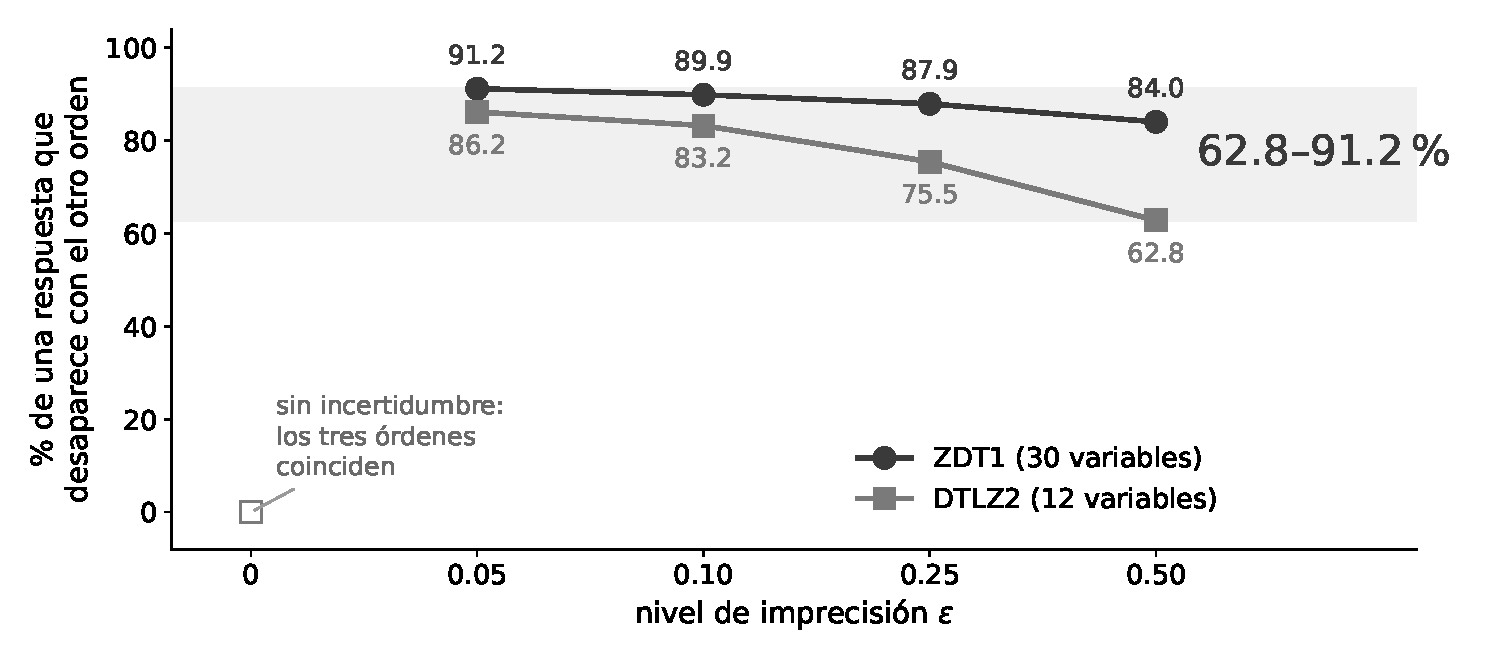
\includegraphics[width=0.98\textwidth,height=0.62\textheight,keepaspectratio]{benchmarks.pdf}
    \end{column}
  \end{columns}
  {\footnotesize Y como sé que mi medida dice que se parecen más de lo que se parecen, esto es un \textbf{mínimo}:
  \\ La diferencia real es mayor.}
  \NotaX
\end{frame}

% ---------------------------------------------------------------- 11
\begin{frame}{Y el tercero no lo he construido yo: está publicado}
  \centering
  \vspace{-2mm}
  {\footnotesize $\IBKone$,\quad $\IBKtwo$,\quad $x\in\IBKbox$}

  \vspace{-1mm}
  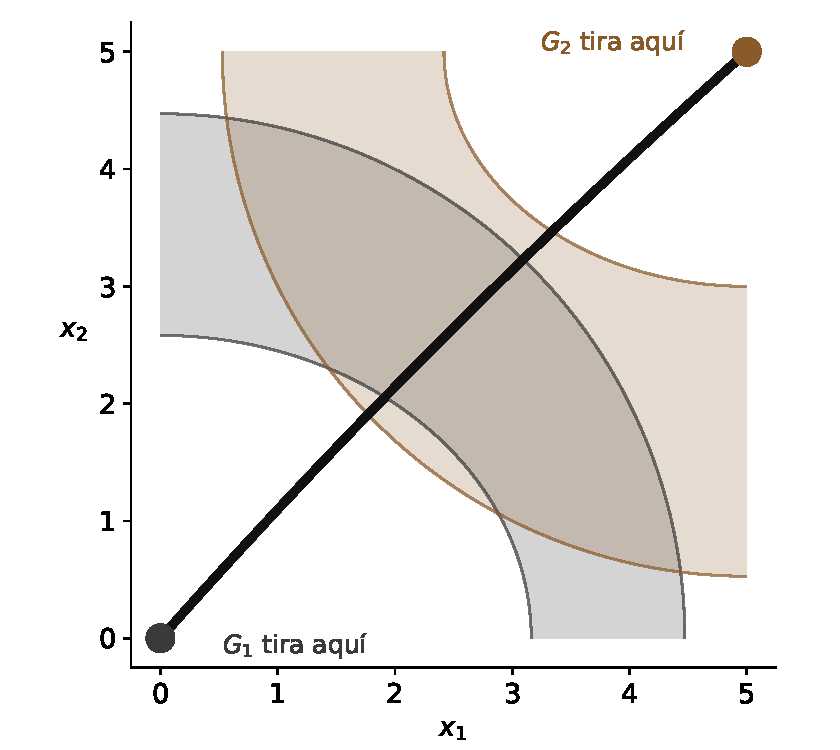
\includegraphics[height=0.69\textheight,keepaspectratio]{ibk1_crisp.pdf}

  \vspace{-1mm}
  {\footnotesize Cada objetivo vale un intervalo.}
  \NotaXI
\end{frame}

% ---------------------------------------------------------------- 12
\begin{frame}{Tres órdenes, tres respuestas: otra vez, y sin tocar el problema}
  \centering
  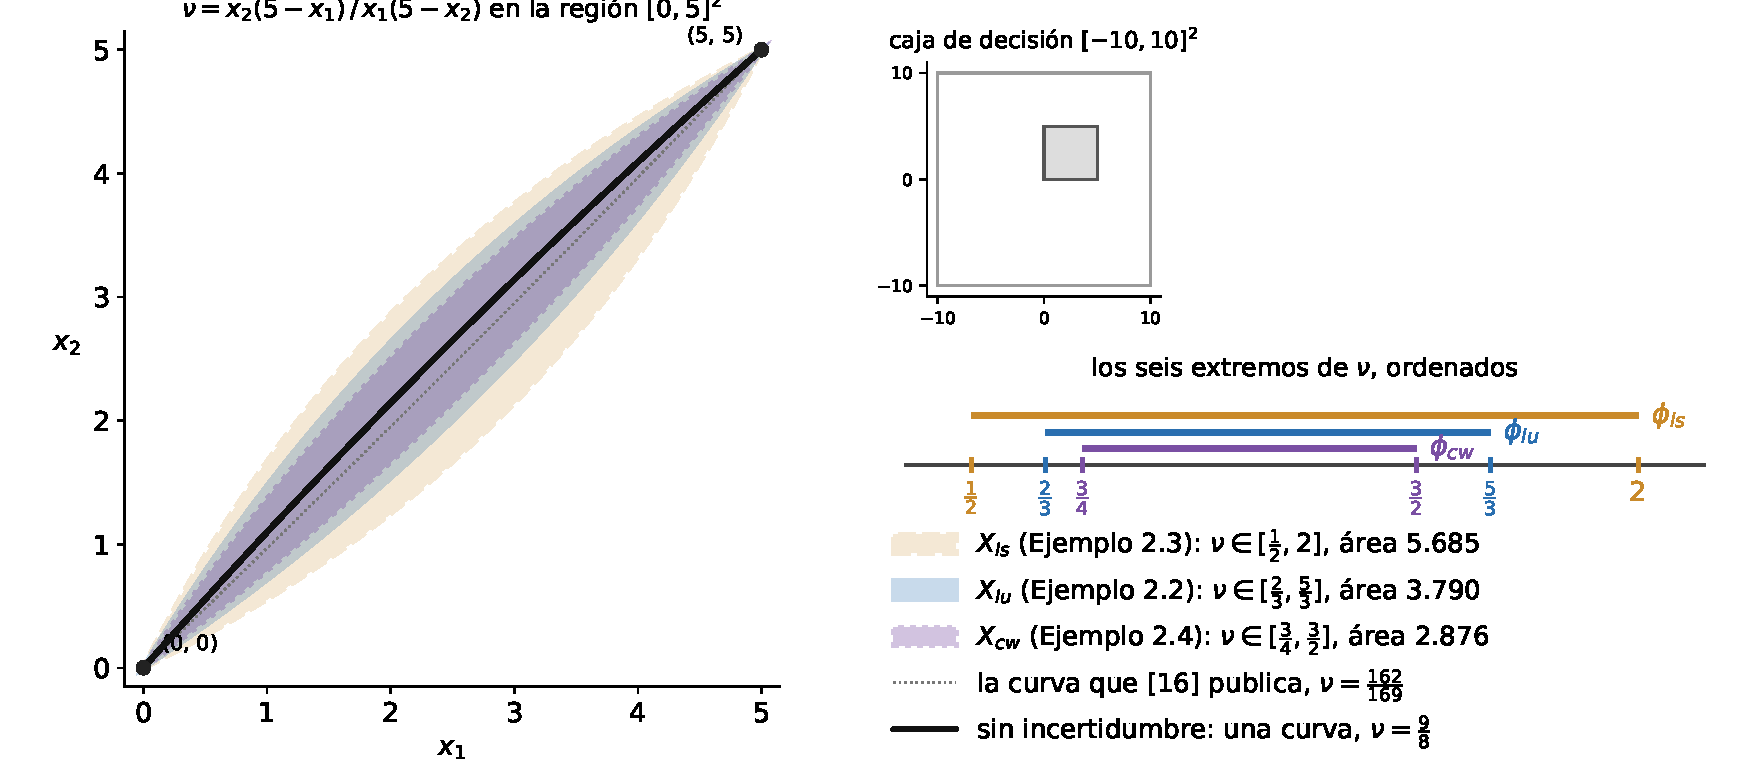
\includegraphics[width=0.98\textwidth,height=0.63\textheight,keepaspectratio]{ibk1_cunas.pdf}

  \vspace{-2mm}
  {\footnotesize Aquí las tres se meten una dentro de otra en vez de cruzarse: el
  \bMinInt--\bMaxInt\,\% de antes no vale aquí.\\ Lo que sí es
  exacto: el \textbf{\iLsOutsideCw\,\%} de la mayor queda fuera de la menor.}
  \NotaXII
\end{frame}

% ---------------------------------------------------------------- 13
\begin{frame}{Y de paso: el punto que publican como óptimo no lo es}
  \centering
  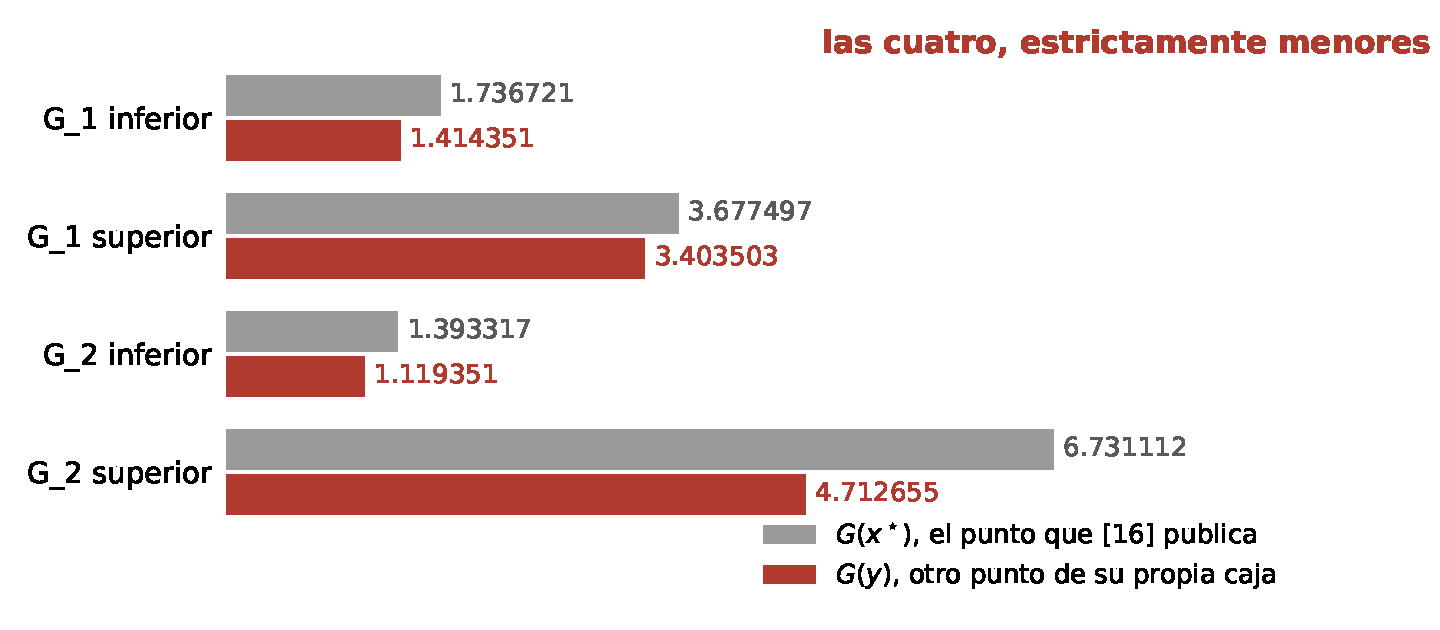
\includegraphics[width=0.88\textwidth,height=0.70\textheight,keepaspectratio]{contraejemplo.pdf}

  \vspace{-1mm}
  {\small Los de arriba son sus números; los de abajo salen con una calculadora
  en dos minutos.\\ \cita{Y los tres algoritmos lo encuentran.}}
  \NotaXIII
\end{frame}

% ---------------------------------------------------------------- cierre
\begin{frame}{Conclusiones}
  \vspace{4mm}
  \begin{center}
    \begin{minipage}{0.88\textwidth}
      {\large Elegir el orden no es un detalle de cómo montas el problema:\\
      \textbf{si no que condiciona la respuesta}.}
    \end{minipage}
  \end{center}
  \vspace{8mm}
  \begin{columns}[T,onlytextwidth]
    \begin{column}{0.32\textwidth}
      \centering
      {\LARGE\textbf{\pUnionShare\,\%}}\\[3mm]
      {\small es todo lo que dos órdenes\\ tienen en común}\\[2mm]
    \end{column}
    \begin{column}{0.32\textwidth}
      \centering
      {\LARGE\textbf{\bMinInt--\bMaxInt\,\%}}\\[3mm]
      {\small de tu respuesta desaparece\\ si te pasas al otro orden}\\[2mm]
    \end{column}
    \begin{column}{0.32\textwidth}
      \centering
      {\LARGE\textbf{\iLsOutsideCw\,\%}}\\[3mm]
      {\small de la respuesta mayor\\ se queda fuera de la menor}\\[2mm]
    \end{column}
  \end{columns}
  \vspace{7mm}
  \begin{center}
    \cita{Y siempre depende del problema: cada cifra viene de un problema concreto.}
  \end{center}
  \NotaXIV
\end{frame}

% ---------------------------------------------------------------- líneas futuras
\begin{frame}{Líneas futuras}
  \vspace{10mm}
  \begin{center}
    \begin{minipage}{0.82\textwidth}
      {\large
      \textbf{La curva de sensibilidad}: ir pasando poco a poco de un orden a
      otro, y ver cómo se mueve la respuesta.\\[8mm]
      \textbf{La aplicación a optimización de carteras}}
    \end{minipage}
  \end{center}
  \NotaXV
\end{frame}

\begin{frame}[plain]
  \vspace{10mm}
  \begin{center}
    {\Huge Gracias}\\[10mm]
  \end{center}
\end{frame}
\end{document}"
%                                                               -> presentacion_notas.pdf
\documentclass[aspectratio=169,11pt]{beamer}

\usetheme[numbering=fraction,progressbar=none,block=fill,background=light]{metropolis}
\usepackage[spanish,es-noshorthands,es-nodecimaldot]{babel}
\usepackage{amsmath,amssymb}
\usepackage{booktabs}
\usepackage{array}
\usepackage{tikz}
\usetikzlibrary{arrows.meta,positioning,calc,patterns,decorations.pathreplacing,shapes.geometric}
\usepackage{pgfpages}
\usepackage{appendixnumberbeamer}

% notas del orador: activadas con \def\shownotes{1} antes de \input
\ifdefined\shownotes
  \setbeameroption{show notes on second screen=right}
  \setbeamertemplate{note page}[plain]
  \setbeamerfont{note page}{size=\scriptsize}
\fi

% ---------------------------------------------------------------- colores
% Los tres órdenes llevan el mismo color en toda la presentación, y son los mismos
% tres valores hexadecimales que experiments/make_presentation.py usa en las
% figuras. Ninguno se lee como bueno o malo. La intersección se raya, nunca lleva
% un cuarto color.
\definecolor{philu}{HTML}{2A6FB0}
\definecolor{phils}{HTML}{C98A2B}
\definecolor{phicw}{HTML}{7A4FA3}
\definecolor{coefcol}{HTML}{B03A2E}
\definecolor{gris}{HTML}{6A6A6A}
\definecolor{grisclaro}{HTML}{DDDDDD}
\setbeamercolor{alerted text}{fg=coefcol}
\setbeamerfont{title}{size=\Large}

\newcommand{\plu}{\textcolor{philu}{$\phi_{lu}$}}
\newcommand{\pls}{\textcolor{phils}{$\phi_{ls}$}}
\newcommand{\pcw}{\textcolor{phicw}{$\phi_{cw}$}}
\newcommand{\Xlu}{\textcolor{philu}{$X_{lu}$}}
\newcommand{\Xls}{\textcolor{phils}{$X_{ls}$}}
\newcommand{\Xcw}{\textcolor{phicw}{$X_{cw}$}}
\newcommand{\coef}[1]{\textcolor{coefcol}{\boldsymbol{#1}}}
\newcommand{\marca}[1]{\textcolor{coefcol}{\boldsymbol{#1}}}
\newcommand{\cita}[1]{\textcolor{gris}{\small #1}}
\newcommand{\refuno}{[1] Costa, Osuna-Gómez y Chalco-Cano (2024)}
\newcommand{\refdieciseis}{[16] Mondal, Ghosh y Kim (2026)}

% ---------------------------------------------------------------- números generados
\graphicspath{{../results/figures/presentation/}}
% generated by experiments/make_presentation.py; do not edit.
% one \newcommand per number, each with the file and key it was read from.
% pRho: src/problems_tier0.py p1_default_params rho
\newcommand{\pRho}{\tfrac{1}{4}}
% pOffset: src/problems_tier0.py p1_default_params, the constant term of the half-width
\newcommand{\pOffset}{\tfrac{1}{8}}
% pBoxLo: src/problems_tier0.py p1_lower
\newcommand{\pBoxLo}{-\tfrac{1}{2}}
% pBoxHi: src/problems_tier0.py p1_upper
\newcommand{\pBoxHi}{\tfrac{3}{2}}
% pAreaLu: results/tier0/exact_regions_p1.csv area,lu
\newcommand{\pAreaLu}{0.311}
% pAreaLs: results/tier0/exact_regions_p1.csv area,ls
\newcommand{\pAreaLs}{1.513}
% pAreaCw: results/tier0/exact_regions_p1.csv area,cw
\newcommand{\pAreaCw}{1.000}
% pUnionShare: results/tier0/exact_regions_p1.csv overlap_union_share,lu,cw (in %)
\newcommand{\pUnionShare}{10.3}
% pLuOutsideCw: results/tier0/exact_regions_p1.csv 1 - coverage_a_in_b,lu,cw (in %)
\newcommand{\pLuOutsideCw}{60.5}
% pCwOutsideLu: results/tier0/exact_regions_p1.csv 1 - coverage_b_in_a,lu,cw (in %)
\newcommand{\pCwOutsideLu}{87.7}
% pCovLuCwExact: results/tier0/exact_regions_p1.csv coverage_a_in_b,lu,cw
\newcommand{\pCovLuCwExact}{0.395}
% pCovCwLuExact: results/tier0/exact_regions_p1.csv coverage_b_in_a,lu,cw
\newcommand{\pCovCwLuExact}{0.123}
% pJacExact: results/tier0/exact_regions_p1.csv overlap_union_share,lu,cw
\newcommand{\pJacExact}{0.103}
% pCovLuCwMeas: results/tier0/instrument_error_p1.csv (lu,cw; delta 0.0; n_evals 5000) measured_median, metric coverage_a_in_b
\newcommand{\pCovLuCwMeas}{0.556}
% pCovLuCwErr: results/tier0/instrument_error_p1.csv (lu,cw; delta 0.0; n_evals 5000) measured/exact, metric coverage_a_in_b
\newcommand{\pCovLuCwErr}{+40.8\,\%}
% pCovLuCwErrLarge: results/tier0/table_2_measured.csv decision block (lu,cw; delta 0.0; n_evals 20000) median/exact, metric coverage_a_in_b
\newcommand{\pCovLuCwErrLarge}{+27.7\,\%}
% pCovCwLuMeas: results/tier0/instrument_error_p1.csv (lu,cw; delta 0.0; n_evals 5000) measured_median, metric coverage_b_in_a
\newcommand{\pCovCwLuMeas}{0.222}
% pCovCwLuErr: results/tier0/instrument_error_p1.csv (lu,cw; delta 0.0; n_evals 5000) measured/exact, metric coverage_b_in_a
\newcommand{\pCovCwLuErr}{+81.0\,\%}
% pCovCwLuErrLarge: results/tier0/table_2_measured.csv decision block (lu,cw; delta 0.0; n_evals 20000) median/exact, metric coverage_b_in_a
\newcommand{\pCovCwLuErrLarge}{+48.6\,\%}
% pJacMeas: results/tier0/instrument_error_p1.csv (lu,cw; delta 0.0; n_evals 5000) measured_median, metric overlap via jaccard = dice/(2-dice)
\newcommand{\pJacMeas}{0.187}
% pJacErr: results/tier0/instrument_error_p1.csv (lu,cw; delta 0.0; n_evals 5000) measured/exact, metric overlap
\newcommand{\pJacErr}{$\times$1.81}
% pJacErrLarge: results/tier0/table_2_measured.csv decision block (lu,cw; delta 0.0; n_evals 20000) median/exact, metric overlap
\newcommand{\pJacErrLarge}{$\times$1.49}
% pJacFactorPlain: results/tier0/instrument_error_p1.csv (lu,cw; delta 0.0; n_evals 5000) jaccard measured/exact
\newcommand{\pJacFactorPlain}{1.81}
% pJacFactorLargePlain: results/tier0/table_2_measured.csv decision block (lu,cw; delta 0.0; n_evals 20000) jaccard measured/exact
\newcommand{\pJacFactorLargePlain}{1.49}
% bMinPct: results/tier1/table_2_measured_eps_{0.05,0.1,0.25,0.5}.csv decision block, lu,cw, finding, coverage_b_in_a, n_evals 5000, delta 0.0: min over the eight cells of 1 - median (in %)
\newcommand{\bMinPct}{62.8}
% bMaxPct: results/tier1/table_2_measured_eps_{0.05,0.1,0.25,0.5}.csv decision block, lu,cw, finding, coverage_b_in_a, n_evals 5000, delta 0.0: max over the eight cells of 1 - median (in %)
\newcommand{\bMaxPct}{91.2}
% bMinInt: results/tier1/table_2_measured_eps_{0.05,0.1,0.25,0.5}.csv decision block, lu,cw, finding, coverage_b_in_a, n_evals 5000, delta 0.0: min, rounded to the integer
\newcommand{\bMinInt}{63}
% bMaxInt: results/tier1/table_2_measured_eps_{0.05,0.1,0.25,0.5}.csv decision block, lu,cw, finding, coverage_b_in_a, n_evals 5000, delta 0.0: max, rounded to the integer
\newcommand{\bMaxInt}{91}
% bZdtVars: src/problems_tier1.py zdt1_n_vars
\newcommand{\bZdtVars}{30}
% bDtlzVars: src/problems_tier1.py dtlz2_n_vars
\newcommand{\bDtlzVars}{12}
% cZdtCardCw: results/tier1/table_2_measured_eps_{0.05,0.1,0.25,0.5}.csv decision block, lu,cw, finding, coverage_b_in_a, n_evals 5000, delta 0.0: cardinality_b, constant over the four eps
\newcommand{\cZdtCardCw}{257}
% cZdtCardLu: results/tier1/table_2_measured_eps_{0.05,0.1,0.25,0.5}.csv decision block, lu,cw, finding, coverage_b_in_a, n_evals 5000, delta 0.0: cardinality_a over eps 0.05, 0.1, 0.25, 0.5
\newcommand{\cZdtCardLu}{26\,\to\,36\,\to\,53\,\to\,68}
% cDtlzCardCw: results/tier1/table_2_measured_eps_{0.05,0.1,0.25,0.5}.csv decision block, lu,cw, finding, coverage_b_in_a, n_evals 5000, delta 0.0: cardinality_b, constant over the four eps
\newcommand{\cDtlzCardCw}{1813}
% cDtlzCardLu: results/tier1/table_2_measured_eps_{0.05,0.1,0.25,0.5}.csv decision block, lu,cw, finding, coverage_b_in_a, n_evals 5000, delta 0.0: cardinality_a over eps 0.05, 0.1, 0.25, 0.5
\newcommand{\cDtlzCardLu}{278\,\to\,351\,\to\,575\,\to\,980}
% ZdtName: src/problems_tier1.py zdt1_interval
\newcommand{\ZdtName}{ZDT1}
% ZdtSize: src/problems_tier1.py zdt1_n_vars, zdt1_n_obj
\newcommand{\ZdtSize}{30 variables, 2 objetivos}
% ZdtF: src/problems_tier1.py evaluate_zdt1, [2] equations (6) and (7)
\newcommand{\ZdtF}{f_1 = x_1, \qquad f_2 = g\,\Bigl(1 - \sqrt{f_1/g}\,\Bigr)}
% ZdtG: src/problems_tier1.py evaluate_zdt1, g with m - 1 = zdt1_n_vars - 1
\newcommand{\ZdtG}{g = 1 + \dfrac{9}{29}\sum_{i \geq 2} x_i}
% ZdtR: src/problems_tier1.py zdt1_half_width
\newcommand{\ZdtR}{r_i = \varepsilon\,\bigl( (\marca{x_d} - \tfrac{1}{2})^2 + \tfrac{1}{20} \bigr)}
% ZdtDrivers: src/problems_tier1.py zdt1_width_drivers, as 1-based names
\newcommand{\ZdtDrivers}{x_{30}, x_{29}}
% DtlzName: src/problems_tier1.py dtlz2_interval
\newcommand{\DtlzName}{DTLZ2}
% DtlzSize: src/problems_tier1.py dtlz2_n_vars, dtlz2_n_obj
\newcommand{\DtlzSize}{12 variables, 3 objetivos}
% DtlzFone: src/problems_tier1.py evaluate_dtlz2, [3] equation (9) at M = 3
\newcommand{\DtlzFone}{f_1 = (1+g)\cos\tfrac{\pi x_1}{2}\cos\tfrac{\pi x_2}{2}}
% DtlzFtwo: src/problems_tier1.py evaluate_dtlz2, [3] equation (9) at M = 3
\newcommand{\DtlzFtwo}{f_2 = (1+g)\cos\tfrac{\pi x_1}{2}\sin\tfrac{\pi x_2}{2}}
% DtlzFthree: src/problems_tier1.py evaluate_dtlz2, [3] equation (9) at M = 3
\newcommand{\DtlzFthree}{f_3 = (1+g)\sin\tfrac{\pi x_1}{2}}
% DtlzG: src/problems_tier1.py evaluate_dtlz2, g over the tail
\newcommand{\DtlzG}{g = \sum_{i \geq 3} (x_i - \tfrac{1}{2})^2}
% DtlzR: src/problems_tier1.py dtlz2_half_width
\newcommand{\DtlzR}{r_i = \varepsilon\,\marca{x_d}}
% DtlzDrivers: src/problems_tier1.py dtlz2_width_drivers, as 1-based names
\newcommand{\DtlzDrivers}{x_{12}, x_{11}, x_{10}}
% IBKone: src/problems_native.py ibk1_coefficients[0]
\newcommand{\IBKone}{G_1 = \coef{[0.1, 0.2]}\, x_1^2 + \coef{[0.1, 0.3]}\, x_2^2}
% IBKtwo: src/problems_native.py ibk1_coefficients[1], ibk1_shift
\newcommand{\IBKtwo}{G_2 = \coef{[0.1, 0.3]}\, (x_1 - 5)^2 + \coef{[0.1, 0.5]}\, (x_2 - 5)^2}
% IBKbox: src/problems_native.py ibk1_lower, ibk1_upper
\newcommand{\IBKbox}{[-10, 10]^2}
% IBKratiosOne: computed from ibk1_coefficients[0]: (b-a)/(a+b) per term
\newcommand{\IBKratiosOne}{\tfrac{1}{3} frente a \tfrac{1}{2}}
% IBKratiosTwo: computed from ibk1_coefficients[1]: (b-a)/(a+b) per term
\newcommand{\IBKratiosTwo}{\tfrac{1}{2} frente a \tfrac{2}{3}}
% iAreaLu: results/part2/exact_regions_ibk1.csv area,lu
\newcommand{\iAreaLu}{3.790}
% iBandLuLo: results/part2/exact_regions_ibk1.csv band_lower,lu
\newcommand{\iBandLuLo}{\tfrac{2}{3}}
% iBandLuHi: results/part2/exact_regions_ibk1.csv band_upper,lu
\newcommand{\iBandLuHi}{\tfrac{5}{3}}
% iAreaLs: results/part2/exact_regions_ibk1.csv area,ls
\newcommand{\iAreaLs}{5.685}
% iBandLsLo: results/part2/exact_regions_ibk1.csv band_lower,ls
\newcommand{\iBandLsLo}{\tfrac{1}{2}}
% iBandLsHi: results/part2/exact_regions_ibk1.csv band_upper,ls
\newcommand{\iBandLsHi}{2}
% iAreaCw: results/part2/exact_regions_ibk1.csv area,cw
\newcommand{\iAreaCw}{2.876}
% iBandCwLo: results/part2/exact_regions_ibk1.csv band_lower,cw
\newcommand{\iBandCwLo}{\tfrac{3}{4}}
% iBandCwHi: results/part2/exact_regions_ibk1.csv band_upper,cw
\newcommand{\iBandCwHi}{\tfrac{3}{2}}
% iOrderedEnds: results/part2/exact_regions_ibk1.csv the six band ends, sorted
\newcommand{\iOrderedEnds}{\tfrac{1}{2} < \tfrac{2}{3} < \tfrac{3}{4} < \tfrac{3}{2} < \tfrac{5}{3} < 2}
% iLsOutsideCw: results/part2/exact_regions_ibk1.csv 1 - coverage_a_in_b,ls,cw (in %)
\newcommand{\iLsOutsideCw}{49.4}
% iCovLsCw: results/part2/exact_regions_ibk1.csv coverage_a_in_b,ls,cw
\newcommand{\iCovLsCw}{0.506}
% iNuCurve: docs/part2/f2_ibk1_derivation.md section 4.1, nu of equation (25)'s curve
\newcommand{\iNuCurve}{\tfrac{162}{169}}
% iCritRatio: docs/part2/f2_ibk1_derivation.md section 4.3, critical set measure over X_lu's
\newcommand{\iCritRatio}{4.24}
% iNuCrisp: computed from src/problems_native.py's coefficients and checked against docs/part2/f2_ibk1_derivation.md section 3.3
\newcommand{\iNuCrisp}{\tfrac{9}{8}}
% IVUone: [16] appendix A problem 2, as docs/part2/f7_ivu2_derivation.md transcribes it
\newcommand{\IVUone}{G_1 = \coef{[1, 1.5]}\, \marca{x_1} + \coef{[1, 1.5]}\, \marca{x_2} + \coef{[1, 1]}}
% IVUtwo: [16] appendix A problem 2, as docs/part2/f7_ivu2_derivation.md transcribes it
\newcommand{\IVUtwo}{G_2 = \coef{[1, 1.5]}\, x_1^2 + \coef{[2, 3]}\, x_2^2 - \coef{[1, 1]}}
% IVUbox: [16] appendix A problem 2, as docs/part2/f7_ivu2_derivation.md transcribes it
\newcommand{\IVUbox}{[-4, 4]^2}
% dXstar: [16] Table 1 page 20, as docs/part2/f2_ibk1_derivation.md section 4.2 (re-computed here in exact rationals from src/problems_native.py's coefficients and asserted equal)
\newcommand{\dXstar}{(3.914930, 1.428474)}
% dY: docs/part2/f2_ibk1_derivation.md section 4.2 (re-computed here in exact rationals from src/problems_native.py's coefficients and asserted equal)
\newcommand{\dY}{(2.8975, 2.3975)}
% dMinMargin: docs/part2/f2_ibk1_derivation.md section 4.2 (re-computed here in exact rationals from src/problems_native.py's coefficients and asserted equal): the smallest of the four margins
\newcommand{\dMinMargin}{0.274}
% dConfigs: results/part2/dominators_summary.csv: number of rows (solver x phi x budget)
\newcommand{\dConfigs}{18}
% dConfigsWithDominator: results/part2/dominators_summary.csv: rows with seeds_with_a_dominator == n_seeds
\newcommand{\dConfigsWithDominator}{18}
% dWidestMargin: results/part2/dominators_summary.csv: max of widest_margin_over_seeds
\newcommand{\dWidestMargin}{0.270}
% iJacFactorMin: results/part2/instrument_error_ibk1.csv, metric overlap, delta 0.0, jaccard = dice/(2-dice), measured/exact over the three pairs (min)
\newcommand{\iJacFactorMin}{1.01}
% iJacFactorMax: results/part2/instrument_error_ibk1.csv, metric overlap, delta 0.0, jaccard = dice/(2-dice), measured/exact over the three pairs (max)
\newcommand{\iJacFactorMax}{1.48}
% aCorrProportional: docs/part1/a1_uncertainty_model.md part 1, the proportional width, corr(centre, width)
\newcommand{\aCorrProportional}{+1.0000}
% rWidthValuesTrue: docs/explicacion_proyecto.md section 10.3
\newcommand{\rWidthValuesTrue}{46}
% rWidthValuesSeen: docs/explicacion_proyecto.md section 10.3
\newcommand{\rWidthValuesSeen}{210}
% rGridPoints: docs/explicacion_proyecto.md section 10.5
\newcommand{\rGridPoints}{40401}
% rFixedCoverage: instrument_error_p1.csv, instrument_error_ibk1.csv, table_2_measured_eps_*.csv: every check row with a containment-fixed direction
\newcommand{\rFixedCoverage}{1.000000}
% rFixedRange: same rows: q3 - q1
\newcommand{\rFixedRange}{0}
% rFixedRows: same rows: how many were checked
\newcommand{\rFixedRows}{28}
% rSatConfigs: results/tier1/rank_one_summary.csv: nsga2 rows with eps > 0 at n_evals 5000
\newcommand{\rSatConfigs}{24}
% rGenerations: results/tier1/rank_one_summary.csv: n_generations
\newcommand{\rGenerations}{50}

% generated by experiments/make_presentation.py from presentation/guion.txt
% one command per slide, in order; presentacion.tex uses them inside \note{}.
\newcommand{\NotaI}{\note{Optimizar es buscar el mejor valor de algo. Con un objetivo hay una respuesta: un punto. En la práctica casi nunca hay uno solo: quieres bajar el coste y bajar el riesgo, y se contradicen. Como optimizar un programa para que sea rápido y gaste poca memoria: no existe el mejor programa. Cuando hay varios objetivos ya no hay un ganador único: hay un conjunto de soluciones que no se pueden mejorar en un objetivo sin empeorar otro. Se llama conjunto eficiente, o frente de Pareto. La regla que lo define es la dominancia, la de la caja. Esto es todo lo que hace falta saber de optimización multiobjetivo}}
\newcommand{\NotaII}{\note{En la realidad no sabemos los valores exactos de las variables. El coste no es 40, es entre 38 y 45: hay un error de medida, hay parámetros que varían, información incompleta. Un intervalo es eso. Tres palabras que hay que fijar ya: centro, semianchura y anchura. Y los objetivos ahora son intervalos, dejan de poder ordenarse. Con A=(1’5 , 5) y =(3,7’5) A parece menor. Pero con A igual a uno a diez y B igual a cuatro a cinco, A puede ser mejor o mucho peor. No hay respuesta. No es un problema técnico: es que no existe una única forma correcta de ordenar intervalos. Existen muchas, y cada una es una decisión sobre qué te importa.}}
\newcommand{\NotaIII}{\note{El primer artículo de Rafaela … , hizo algo elegante: en vez de proponer un orden, describió toda la familia de órdenes posibles, con un parámetro que dice cuál estás usando. Ese parámetro es fi. Un fi coge un intervalo y devuelve dos números reales, que sí se pueden comparar. Los tres que el artículo nombra: fi\_Lu, compara mejor caso con mejor caso y peor con peor fi\_Ls, extremo inferior y anchura; fi\_cw, centro y semianchura. Los tres son válidos, distintos, y cada uno da un conjunto eficiente distinto. Analogía: fi es la función clave de un sort. La regla: m objetivos intervalares se convierten en dos m objetivos reales, y eso ya se sabe resolver con NSGA-II o PSO. El artículo demuestra que resolver el transformado equivale a resolver el original}}
\newcommand{\NotaIV}{\note{Y con esto ya puedo decir qué es lo que me pregunto, que es una sola cosa: si cambio el orden y no cambio nada más, ¿cambia la respuesta? ¿Y cuánto? Hay otra pregunta que la gente hace enseguida y que yo no contesto: cuál de los tres órdenes es el bueno. No la contesto porque no se puede con lo que tengo delante. Cada orden mira el problema a su manera, y para decir cuál acierta haría falta saber qué pasa de verdad después, en la realidad. Estos problemas de prueba no lo dicen. Prefiero decirlo yo ahora y no que se quede la duda.}}
\newcommand{\NotaV}{\note{Lo primero que hice fue lo obvio, y salió mal. Es el hallazgo del que más he aprendido. Cogí un problema normal y le puse un margen de error fijo arriba y abajo: en vez de un número, un intervalo de ancho siempre igual. Parece sensato y es inútil. Si todos los intervalos tienen el mismo ancho, dos de los tres órdenes están mirando un número que nunca cambia. Y un dato que es siempre el mismo no sirve para ordenar nada: es como ordenar una lista de gente por el número siete. Resultado: los tres órdenes daban exactamente el mismo conjunto, y encima el mismo que si no hubiera incertidumbre. Y no lo deduje, lo medí: los tres conjuntos salieron con los mismos puntos, uno por uno. De aquí sale la regla que gobierna todo lo demás: la incertidumbre tiene que depender de algo que el valor central no controle. Si el ancho se puede calcular a partir del centro, los tres órdenes se vuelven el mismo. Si hubiera montado el estudio sin darme cuenta de esto, todas mis tablas habrían salido llenas de unos y habría concluido que el orden da igual. Que es justo lo contrario de la verdad.}}
\newcommand{\NotaVI}{\note{Antes de enseñaros lo que sale, un minuto con el problema, porque si no la siguiente imagen no se entiende. Me construí un problema de dos variables, a medida, para poder resolverlo a mano. Los dos objetivos son lo mismo: acércate a un punto. Uno te pide acercarte a éste y el otro a éste de aquí. Si sólo tuviera el primero, la respuesta sería ese punto, y ya está. Si sólo tuviera el segundo, el otro. Pero no puedo estar en los dos sitios a la vez. Y fijaos en lo que pasa con cualquier punto que no esté en la línea: si tiro hacia la línea me acerco a los dos objetivos a la vez, así que ese punto no puede ser una respuesta, porque hay otro mejor en todo. Conclusión: sin incertidumbre, la respuesta de este problema es exactamente el segmento que une los dos puntos. Una línea. Quedaos con esa línea, porque ahora le voy a meter la incertidumbre y vamos a ver qué le pasa.}}
\newcommand{\NotaVII}{\note{Así que me construí un problema a medida, con dos variables, para poder resolverlo a mano. Tiene dos objetivos, y la gracia está en el cruce: la incertidumbre de cada objetivo depende de la variable del otro. Que es la regla de antes, aplicada. Y como todo es cuadrático, las condiciones de optimalidad se convierten en un sistema de ecuaciones que se resuelve con papel y lápiz. Usando el Teorema 3.3 y el Ejemplo 3.9 del artículo de Rafaela — sus propios resultados, aplicados, no inventados por mí — saco la respuesta exacta bajo cada uno de los tres órdenes. Y esto es lo que sale. Esto no es lo que me ha devuelto un ordenador: son las tres fórmulas dibujadas. No hay muestreo ni algoritmo dentro. Los dos ejes son las dos variables. El cuadrado es la respuesta con un orden, la región grande con otro, la lente con el tercero. Mismo problema, mismos datos; lo único que cambia es el orden. Y mirad lo que pasa: la lente y el cuadrado no se contienen. La lente sube por arriba, donde el cuadrado no llega; el cuadrado ocupa todo lo de abajo, donde la lente no llega. Cada uno tiene una zona a la que el otro no alcanza. De todo lo que podrían tener en común, sólo comparten el diez por ciento. Y esto es exacto, medido sobre las fórmulas. Si alguien está eligiendo entre soluciones, cambiar de orden le cambia casi toda la lista.}}
\newcommand{\NotaVIII}{\note{Ahora, en un problema así yo tengo la respuesta exacta. Pero en un problema de verdad no la voy a tener: voy a tener lo que me devuelva el ordenador. Así que aproveché: tengo las dos cosas a la vez, lo exacto y lo medido, y las puse una al lado de la otra. Esto es algo que casi ningún trabajo tiene: sé cuánto se equivoca mi propio instrumento. Y se equivoca siempre en la misma dirección: dice que los dos órdenes se parecen más de lo que se parecen. Donde de verdad comparten un diez por ciento, él dice dieciocho. La razón es fácil de ver: cuando pruebas puntos al azar, encuentras primero los fáciles, y los fáciles son justo los que están en la zona común. Lo que pertenece a un solo conjunto está en los bordes y cuesta más pillarlo. Ese factor, casi el doble, es de este problema. No lo llevo a ningún otro sitio ni corrijo ningún número con él.}}
\newcommand{\NotaIX}{\note{Hasta aquí todo ha sido un problema de dos variables que me inventé yo. Toca salir a problemas de verdad. Éstos son dos de los que se usan como referencia en el campo: ZDT1 y DTLZ2. No son míos: están publicados y todo el mundo los conoce. El primero tiene treinta variables y dos objetivos, y su respuesta, sin incertidumbre, es esa curva. El segundo tiene doce variables y tres objetivos, y su respuesta es ese trozo de esfera. Fijaos en el salto: antes la respuesta era un segmento en un plano que cabía en una imagen; aquí ya no puedo dibujar el espacio de las soluciones, porque tiene treinta dimensiones. A los dos les pongo una banda de incertidumbre encima, con la regla del principio: la anchura la mueve una variable que no está en el centro. Está marcada en rojo. Y el parámetro épsilon es cuánta imprecisión les meto. Voy a probar cuatro niveles.}}
\newcommand{\NotaX}{\note{Aquí está el método, y es lo que hace que el número de la derecha valga algo. Va de arriba abajo, por el esquema de la izquierda. Uno: cojo cinco mil puntos al azar dentro de la caja. Al azar de verdad, sin mirar los objetivos y sin usar nada de lo que sé del problema. Dos: evalúo esos cinco mil puntos una sola vez. Cada punto me devuelve sus intervalos, uno por objetivo, y esa lista ya no se vuelve a tocar. Tres: cojo esa única lista y la filtro tres veces. En cada pasada uso uno de los tres órdenes: comparo los puntos entre sí con ese criterio y me quedo con los que no domina nadie. Tres pasadas sobre la misma lista, tres subconjuntos. Y aquí está la gracia: los tres salen de los mismos puntos y de los mismos números; lo único distinto es el criterio con el que comparo. Así que cualquier diferencia entre ellos es del orden y de nada más. Si lanzara un algoritmo evolutivo tres veces, una con cada orden, cambiaría dos cosas a la vez: el criterio, que es lo que quiero medir, y por dónde busca el algoritmo. Saldrían mezcladas y no podría separarlas. Por eso probar al azar no es el rival flojo: es el instrumento con el que mido. NSGA-II y el PSO multiobjetivo sí están en el trabajo, pero en otro sitio: comprobando que los solvers llegan a donde la derivación dice, y en la última diapositiva. Y esto es lo que sale: entre el sesenta y tres y el noventa y uno por ciento de lo que te daba un orden desaparece si te pasas al otro. Y como ya sé que mi instrumento exagera el parecido, esto es un mínimo: la diferencia real es mayor. No están inflados a mi favor, sino en mi contra. Abajo a la izquierda, la comprobación: sin incertidumbre, los tres órdenes vuelven a dar lo mismo.}}
\newcommand{\NotaXI}{\note{Llegados aquí alguien puede decirme, con toda la razón: claro, te has construido tú el problema para que salga lo que querías. Y es verdad, y por eso está medido y escrito. Así que el tercer problema no lo he tocado yo. Está publicado por otros autores, para otra cosa, antes de que yo empezara. Y es intervalar de origen: los intervalos están en los propios coeficientes, ahí arriba, entre corchetes. Yo no elegí ni cuánto valen ni de qué variable dependen. Por dentro es el mismo tipo de problema que el mío: dos objetivos, y cada uno te pide acercarte a una esquina. Uno tira hacia el cero y el otro hacia el cinco cinco. Con una diferencia que se ve en el dibujo: como los coeficientes son intervalos, un objetivo ya no vale un número. Pedirle que valga dos no te da una curva, te da esa banda sombreada. Y como antes: si quito la incertidumbre y me quedo con los valores centrales, la respuesta es una sola curva, la negra. Quedaos otra vez con esa curva.}}
\newcommand{\NotaXII}{\note{Y esto es lo que sale al derivarlo a mano, que es más bonito de lo que esperaba: toda la respuesta cabe en un solo número. Cada orden se queda con los puntos cuyo número cae dentro de un intervalo, y el intervalo depende del orden. Tres cuñas, ancladas en las mismas dos esquinas, con la curva de antes por el medio. Otra vez tres órdenes, tres respuestas distintas, en un problema que no es mío. Y fijaos en el salto: sin incertidumbre era una curva; con cada orden es una región con superficie. Pero aquí tengo que ser honesto con una cosa: estas tres se meten una dentro de otra, no se cruzan como antes. Así que el número del sesenta y tres al noventa y uno no tiene equivalente aquí, y no lo reclamo. Lo que sí puedo decir es que la mitad de la mayor se queda fuera de la menor. Y hay una comprobación que no es mía y que sale bien: ellos publican una curva de soluciones, la calculo, y cae dentro de las tres cuñas. Un apunte más, porque marca el límite: derivé un segundo problema suyo y ahí los tres órdenes dan exactamente lo mismo. O sea que ser un problema intervalar de verdad no basta para que el orden importe. Se sabe mirando los coeficientes, antes de resolver nada.}}
\newcommand{\NotaXIII}{\note{Y esto salió de paso. No me puse a buscar errores en nadie: me puse a comprobar mi propia derivación contra lo que ellos publican, que es lo que hay que hacer. Ellos dan este punto como solución óptima de su problema. Su propia definición dice qué significa eso: que no exista otro punto que sea igual o mejor en las cuatro cantidades. Cogí otro punto, que está dentro de su misma caja, y lo comparé con los números que ellos imprimen. Las cuatro salen menores. Las cuatro. Los de arriba son sus números, tal como están en el artículo; los de abajo se calculan con una calculadora en dos minutos. No hace falta creerse nada de lo que yo he hecho. Y no es cosa del redondeo: la diferencia más ajustada es doscientas mil veces mayor que lo que podría moverse el último decimal que ellos imprimen. Además, los tres algoritmos lo encuentran solos. A la sesión que los lanzó no se le dijo nada de este punto, y las dieciocho configuraciones devolvieron puntos que lo ganan. Es una corrección, no una crítica. Y lo que no digo es dónde está el fallo de su demostración: se apoya en otro artículo suyo que yo no tengo. Digo que la conclusión es falsa; no digo por qué.}}
\newcommand{\NotaXIV}{\note{Y resumo con lo que defiendo, que es una sola cosa: elegir el orden no es un detalle de cómo montas el problema, es media respuesta. Con tres medidas. En mi problema, hecho a mano y exacto: de todo lo que podrían tener en común dos órdenes, sólo comparten el diez por ciento. En dos problemas de referencia del campo, medido: entre el sesenta y tres y el noventa y uno por ciento de lo que te daba un orden desaparece si te pasas al otro. Y con un instrumento cuyo error conozco, así que eso es un mínimo. Y en un problema publicado por otros, que no he tocado yo: la mitad de la respuesta mayor se queda fuera de la menor. Todo esto bajo una condición sobre el modelo de incertidumbre que no supuse, sino que medí, y que además se puede comprobar en cualquier problema antes de ponerse a resolver. Y tres cosas que no sé, y que están escritas: por qué a uno de los algoritmos le cuesta más de lo que debería, después de descartar cinco explicaciones midiéndolas; por qué en un problema las respuestas se cruzan y en otro se anidan; y por qué mi instrumento se equivoca casi el doble en un problema y casi nada en otro. Que esas tres estén escritas es parte del resultado, no un defecto.}}
\newcommand{\NotaXV}{\note{Y lo que queda por hacer, que son dos cosas. La primera es la curva de sensibilidad: en vez de tres órdenes sueltos, ir pasando poco a poco de uno a otro y ver cómo se mueve la respuesta. Es admisible por la propia definición del artículo y el código está montado para que sea un bucle; fue lo primero que me quité de encima por falta de tiempo, y es la mejora más grande que hay disponible. Y la segunda son las carteras, que es donde vuestra propia propuesta las pone, como trabajo futuro. Gracias.}}


\title{Técnicas de Optimización Intervalar basadas en Inteligencia Computacional}
\subtitle{¿Cuánto cambia la respuesta cuando lo único que cambia es el orden?}
\author{Francisco Rodríguez-Carretero Roldán}
\institute{Tutores: Antonio Beato Moreno y Rafaela Osuna Gómez · Universidad de Sevilla}
\date{25 de septiembre de 2026 · Proyecto PI3, julio--septiembre 2026}

\begin{document}

% ================================================================ portada
\begin{frame}[plain]
  \vspace{-6mm}\titlepage
\end{frame}

% ================================================================ BLOQUE A
% ---------------------------------------------------------------- 1
\begin{frame}{Optimizar con varios objetivos: no hay un ganador, hay un conjunto}
  \begin{columns}[T]
    \begin{column}{0.52\textwidth}
      \centering
      \begin{tikzpicture}[scale=0.55]
        \draw[-{Stealth}] (0,0) -- (10.5,0) node[below left] {coste};
        \draw[-{Stealth}] (0,0) -- (0,9.5) node[below right,rotate=0] {riesgo};
        % dominados
        \foreach \x/\y in {3/7, 5/6, 6/4.5, 8/4, 4/6.5, 7/3.5, 9/5, 2.5/8.5, 5.5/8, 8.5/6.5, 3.5/5.5, 6.5/6}
          \fill[gris!60] (\x,\y) circle (0.14);
        % no dominados
        \draw[dashed,gris] plot[smooth] coordinates {(1,8) (2,5.5) (3.5,4) (5,3) (7,2.2) (9,1.8)};
        \foreach \x/\y in {1/8, 2/5.5, 3.5/4, 5/3, 7/2.2, 9/1.8}
          \fill[philu] (\x,\y) circle (0.2);
        \node[philu,align=left,font=\small] at (7.6,7.8) {conjunto eficiente\\(frente de Pareto)};
        \node[gris,font=\small] at (6.2,1.2) {dominados};
      \end{tikzpicture}
    \end{column}
    \begin{column}{0.46\textwidth}
      Bajar el coste sube el riesgo: no hay una solución única, existe un conjunto
      de soluciones eficientes.
      \begin{block}{Dominancia}
        $A$ domina a $B$ si $A$ es igual o mejor que $B$ en \textbf{todos} los
        objetivos y estrictamente mejor en \textbf{al menos uno}.
      \end{block}
      \vspace{2mm}
      Una solución es \textbf{eficiente} si nadie la domina.\\[2mm]
    \end{column}
  \end{columns}
  \NotaI
\end{frame}

% ---------------------------------------------------------------- 2
\begin{frame}{Bajo incertidumbre, los intervalos no siempre se ordenan intuitivamente}
  \centering
  \begin{tikzpicture}[scale=0.66]
    % el intervalo [38, 45]
    \begin{scope}
      \draw[thick] (0,0) -- (7,0);
      \draw[very thick,philu] (1,0) -- (6,0);
      \draw[very thick,philu] (1,-0.15) -- (1,0.15) node[above] {$38$};
      \draw[very thick,philu] (6,-0.15) -- (6,0.15) node[above] {$45$};
      \fill[philu] (3.5,0) circle (0.07) node[above,text=black] {centro $41.5$};
      \draw[decorate,decoration={brace,mirror,amplitude=4pt}] (1,-0.3) -- (3.5,-0.3)
        node[midway,below=4pt,font=\small,text=black] {semianchura $3.5$};
      \draw[decorate,decoration={brace,mirror,amplitude=4pt}] (1,-1.1) -- (6,-1.1)
        node[midway,below=4pt,font=\small,text=black] {anchura $7$};
      \node[right,font=\small,gris,align=left,text width=4.8cm] at (7.6,0.2) {``el coste no es $40$, es $[38, 45]$''};
    \end{scope}
    % A = [1.5, 5], B = [3, 7.5]
    \begin{scope}[yshift=-4.6cm]
      \draw[-{Stealth}] (0,0) -- (10,0) node[right] {$\mathbb{R}$};
      \foreach \x in {0,1,...,9} \draw (\x,-0.08) -- (\x,0.08) node[below=2pt,font=\scriptsize] {\x};
      \draw[very thick,philu] (1.5,0.5) -- (5,0.5) node[midway,above,font=\small] {$A = [1.5, 5]$};
      \draw[very thick,phicw] (3,1.5) -- (7.5,1.5) node[midway,above,font=\small] {$B = [3, 7.5]$};
      \node[right,font=\small,align=left,text width=4.8cm] at (10.6,0.9) {$A$ empieza y acaba antes:\\ aquí $A$ parece menor.};
    \end{scope}
    \begin{scope}[yshift=-8.2cm]
      \draw[-{Stealth}] (0,0) -- (10,0) node[right] {$\mathbb{R}$};
      \foreach \x in {0,1,...,9} \draw (\x,-0.08) -- (\x,0.08);
      \draw[very thick,philu] (1,0.5) -- (10,0.5) node[midway,above,font=\small] {$A = [1, 10]$};
      \draw[very thick,phicw] (4,1.5) -- (5,1.5) node[midway,above,font=\small] {$B = [4, 5]$};
      \node[right,font=\small,align=left,text width=4.8cm] at (10.6,0.9) {\textbf{¿Cuál es menor?}\\ No hay respuesta.};
    \end{scope}
  \end{tikzpicture}
  \NotaII
\end{frame}

% ---------------------------------------------------------------- 3
\begin{frame}{Una familia entera de órdenes, con un parámetro que dice cuál usas: $\phi$}
  \begin{columns}[c,onlytextwidth]
    \begin{column}{0.27\textwidth}
      \centering
      \begin{tikzpicture}[node distance=3.5mm,every node/.style={font=\small}]
        \node[draw,rounded corners,minimum height=7mm] (in) {$[\,l,\,u\,]$};
        \node[draw,rounded corners,fill=grisclaro,minimum height=7mm,right=of in] (phi) {$\phi$};
        \node[draw,rounded corners,minimum height=7mm,right=of phi] (out) {$(a,\,b)$};
        \draw[-{Stealth}] (in) -- (phi);
        \draw[-{Stealth}] (phi) -- (out);
      \end{tikzpicture}\\[1mm]
      {\small\color{gris} dos reales sí se comparan}
    \end{column}
    \begin{column}{0.71\textwidth}
      \footnotesize\setlength{\tabcolsep}{4pt}
      \begin{tabular}{@{}lll@{}}
        \toprule
        orden & fórmula & qué mira \\
        \midrule
        \plu\ (Ejemplo 2.2) & $[l,u]\mapsto(l,\;u)$ & inferior y superior \\
        \pls\ (Ejemplo 2.3) & $[l,u]\mapsto(l,\;u-l)$ & inferior y \textbf{anchura} \\
        \pcw\ (Ejemplo 2.4) & $[l,u]\mapsto\bigl(\tfrac{l+u}{2},\;\tfrac{u-l}{2}\bigr)$ & centro y \textbf{semianchura} \\
        \bottomrule
      \end{tabular}
    \end{column}
  \end{columns}
  \vspace{4mm}
  \begin{columns}[T]
    \begin{column}{0.48\textwidth}
      \begin{block}{La analogía}
        $\phi$ es la función \texttt{key} de un \texttt{sort}: cambias la
        \texttt{key}, cambia el orden.
      \end{block}
    \end{column}
    \begin{column}{0.48\textwidth}
      \begin{block}{La regla}
        $m$ objetivos intervalares $\to$ $2m$ objetivos reales, y un problema
        real ya se sabe resolver.
      \end{block}
    \end{column}
  \end{columns}
  \vspace{2mm}
  \cita{Ejemplos 2.2, 2.3 y 2.4 de \refuno. Los tres son válidos}
  \NotaIII
\end{frame}

% ---------------------------------------------------------------- 4
\begin{frame}{}
  \vspace{8mm}
  \begin{center}
    {\LARGE\bfseries Si cambio el orden y no cambio nada más,\\[3mm]
     ¿cambia la respuesta? ¿Y cuánto?}
  \end{center}
\end{frame}

% ---------------------------------------------------------------- 5
\begin{frame}{Lo primero que probé fue lo obvio, y no medía nada}
  \centering
  \begin{tikzpicture}[scale=0.82,font=\scriptsize]
    \begin{scope}
      \draw[-{Stealth},gris] (0,-0.4) -- (4.4,-0.4);
      \fill[gris!25] plot[smooth,domain=0.3:4.1] ({\x},{1.5-0.35*\x+0.09*\x*\x+0.45})
        -- plot[smooth,domain=4.1:0.3] ({\x},{1.5-0.35*\x+0.09*\x*\x-0.45}) -- cycle;
      \draw[very thick,philu] plot[smooth,domain=0.3:4.1] ({\x},{1.5-0.35*\x+0.09*\x*\x});
      \draw[<->,coefcol,thick] (3.1,{1.5-0.35*3.1+0.09*3.1*3.1-0.45}) -- (3.1,{1.5-0.35*3.1+0.09*3.1*3.1+0.45})
        node[midway,right=1.2mm,coefcol] {$2\varepsilon$};
      \node[gris,font=\scriptsize,align=center] at (2.2,-1.25) {un margen de error \textbf{siempre igual}};
    \end{scope}
    \begin{scope}[xshift=5.6cm,yshift=1.3cm,font=\small]
      \node[philu] at (0,0.8) {\plu};
      \node[phils] at (0,0) {\pls};
      \node[phicw] at (0,-0.8) {\pcw};
      \node[anchor=west] at (0.4,0.8) {$(f-\varepsilon,\; f+\varepsilon)$};
      \node[anchor=west] at (0.4,0) {$(f-\varepsilon,\; \coef{2\varepsilon})$};
      \node[anchor=west] at (0.4,-0.8) {$(f,\; \coef{\varepsilon})$};
      \node[coefcol,font=\scriptsize,align=center] at (1.6,-1.6) {nunca cambian};
    \end{scope}
    \begin{scope}[xshift=11.2cm,yshift=1.3cm,font=\scriptsize]
      \draw[very thick,phils,fill=phils!12] (0,0) circle (1.25);
      \draw[very thick,philu,dashed] (0,0) circle (1.25);
      \draw[very thick,phicw,dotted] (0,0) circle (1.25);
      \node[align=center] at (0,0) {los tres dan\\la misma\\respuesta};
    \end{scope}
    \draw[-{Stealth},gris,thick] (9.3,1.3) -- (9.8,1.3);
  \end{tikzpicture}

  \vspace{1mm}
  \begin{minipage}{0.84\textwidth}
    \begin{block}{La regla que saqué de aquí}
      La incertidumbre tiene que depender de algo que el valor central no
      controle. Si el ancho se puede calcular a partir del centro, los tres
      órdenes se vuelven el mismo.
    \end{block}
  \end{minipage}
  \NotaV
\end{frame}

% ---------------------------------------------------------------- 6
\begin{frame}{El problema p1, sin incertidumbre todavía: acercarse a dos sitios a la vez}
  \centering
  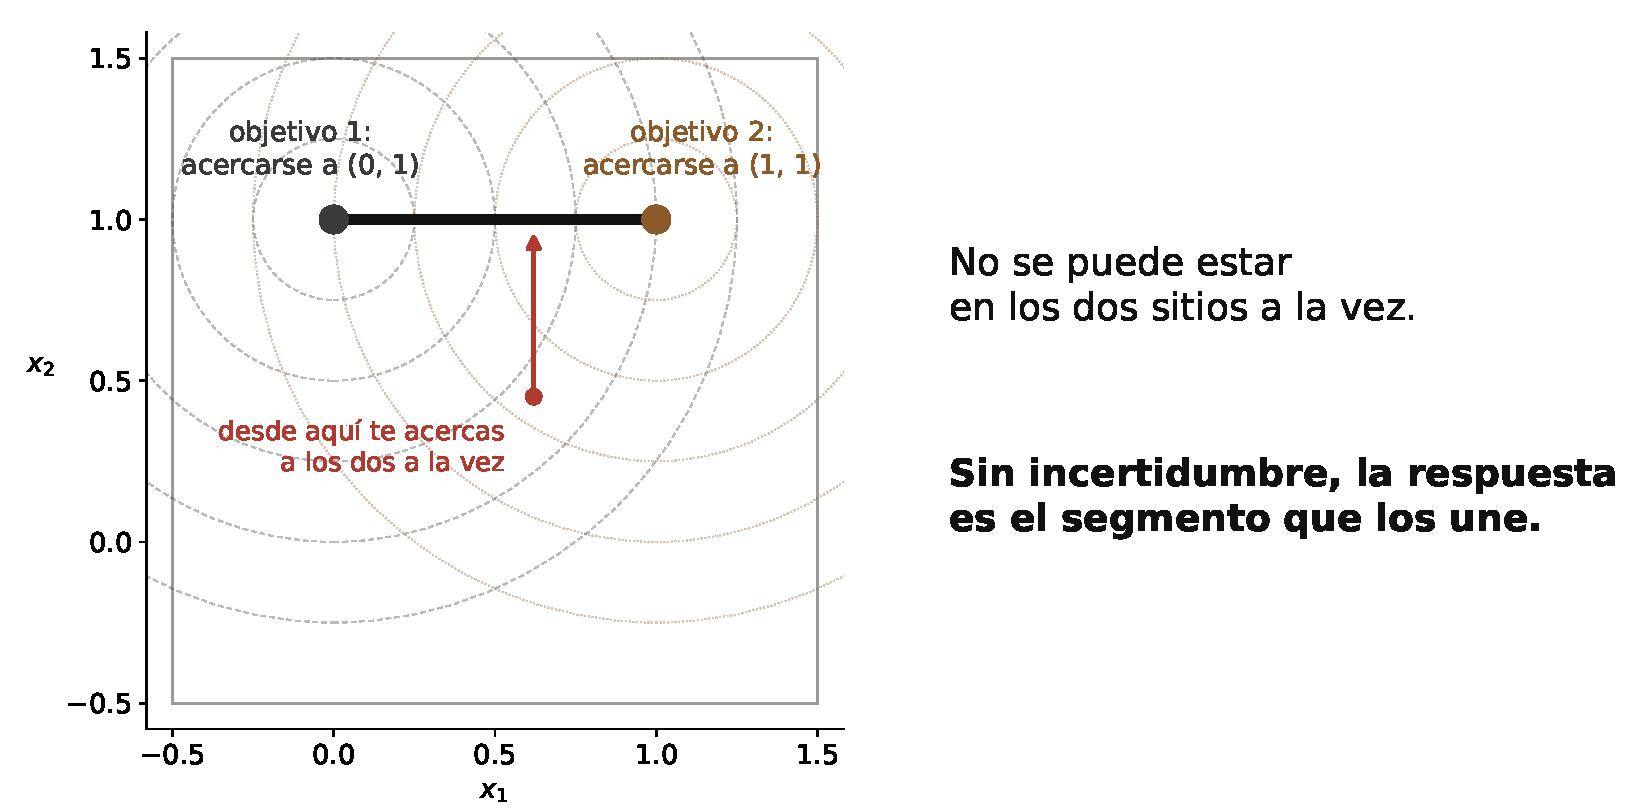
\includegraphics[width=0.99\textwidth,height=0.70\textheight,keepaspectratio]{p1_crisp.pdf}

  \vspace{-2mm}
  {\footnotesize Dos variables, un problema que se puede resolver a mano.}
  \NotaVI
\end{frame}

% ---------------------------------------------------------------- 7
\begin{frame}{p1, tres órdenes, tres respuestas distintas}
  \centering
  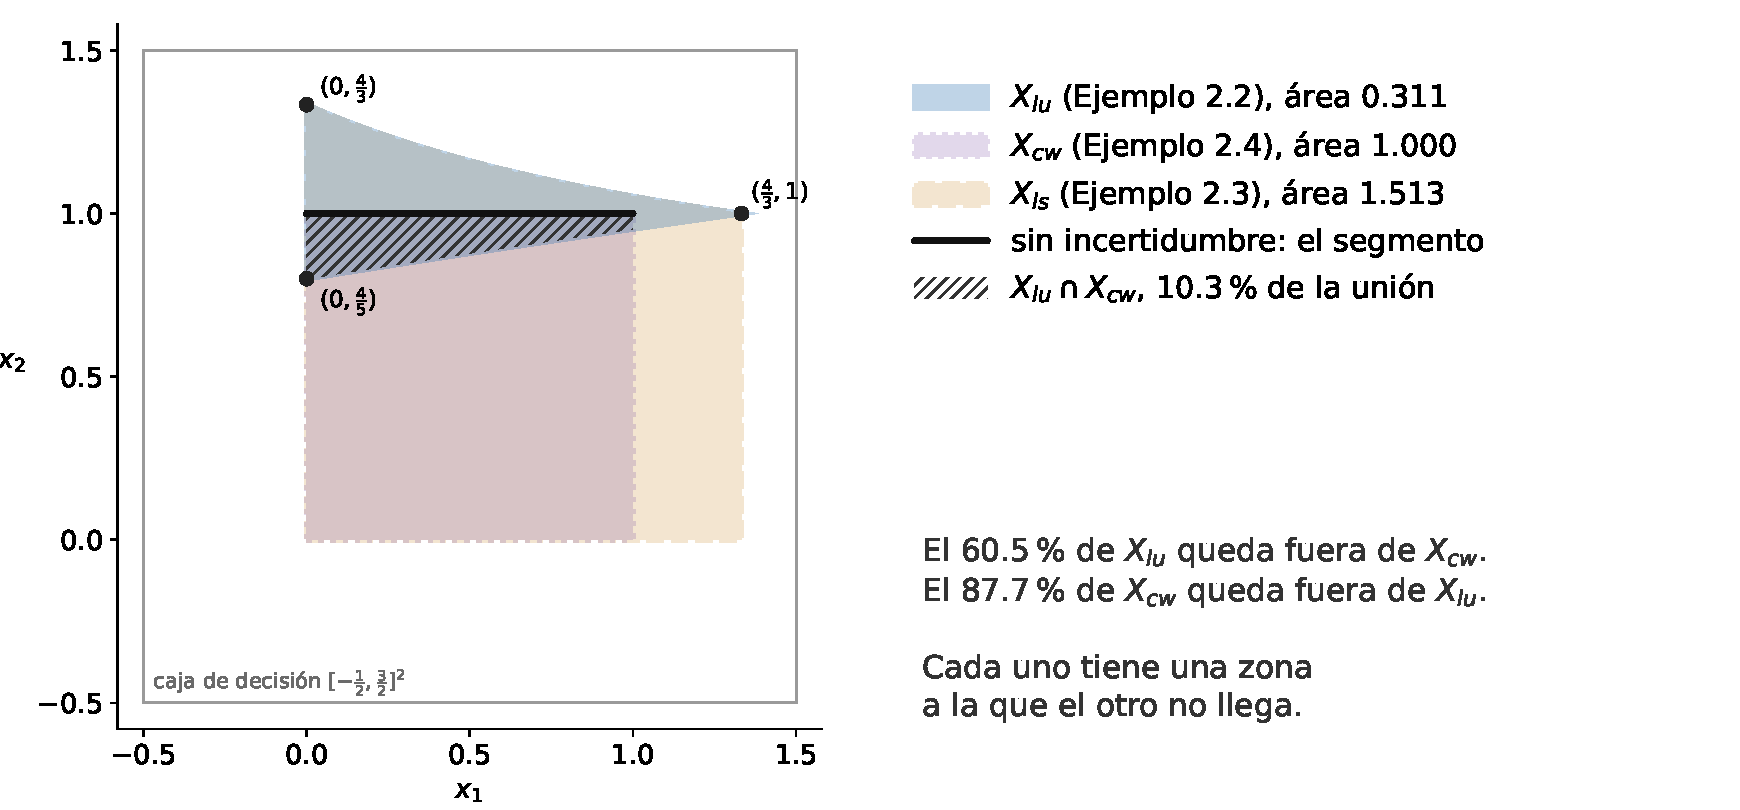
\includegraphics[width=0.98\textwidth,height=0.70\textheight,keepaspectratio]{p1_regiones.pdf}

  \vspace{-2mm}
  {\footnotesize De todo lo que podrían tener en común, sólo comparten el
  \textbf{\pUnionShare\,\%}. \cita{Y esto no lo ha calculado un ordenador: son las tres fórmulas dibujadas.}}
  \NotaVII
\end{frame}

% ---------------------------------------------------------------- 8
\begin{frame}{Y sé cuánto se equivoca lo que uso para medir}
  \centering
  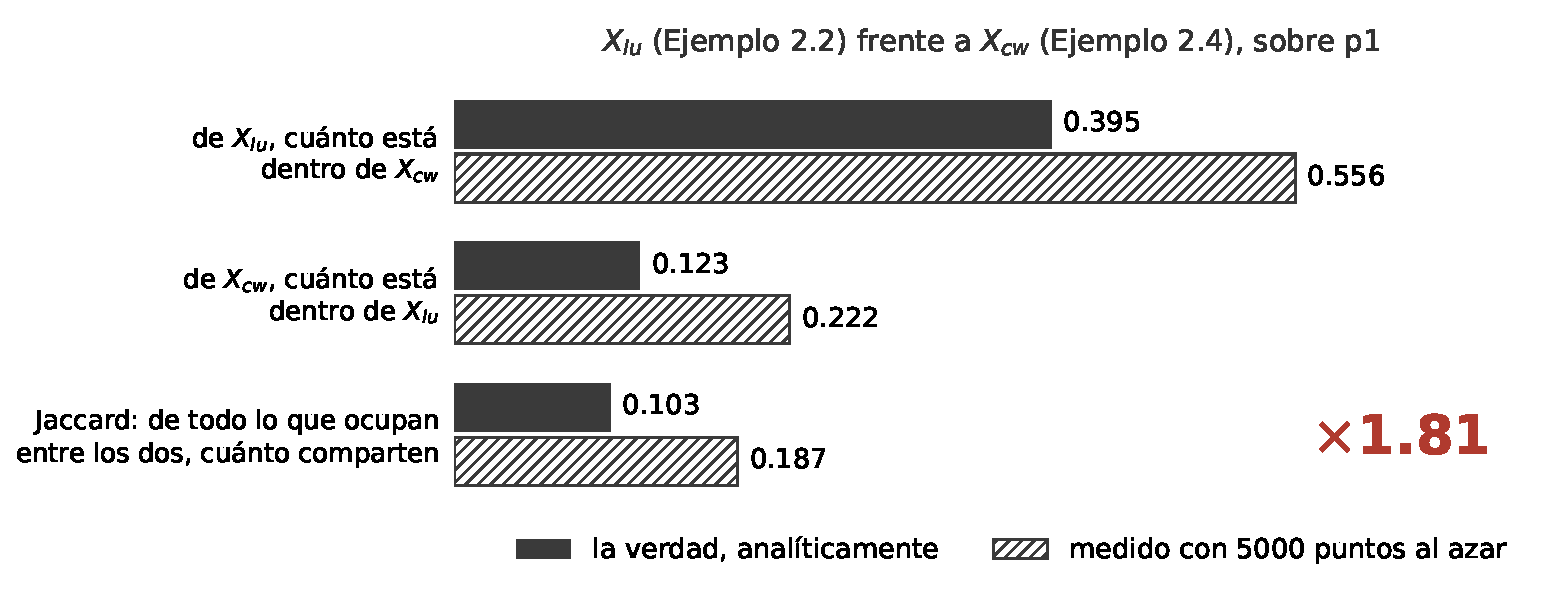
\includegraphics[width=0.97\textwidth,height=0.68\textheight,keepaspectratio]{instrumento.pdf}

  \vspace{-1mm}
  {\small Siempre en la misma dirección: al medir con puntos al azar, los dos
  órdenes salen \textbf{más parecidos de lo que son}.}
  \NotaVIII
\end{frame}

% ---------------------------------------------------------------- 9
\begin{frame}{Y ahora, p2, problemas de referencia del campo}
  \begin{columns}[T,onlytextwidth]
    \begin{column}{0.49\textwidth}
      \centering
      {\large\textbf{\ZdtName}} \quad \cita{\ZdtSize}\\[1mm]
      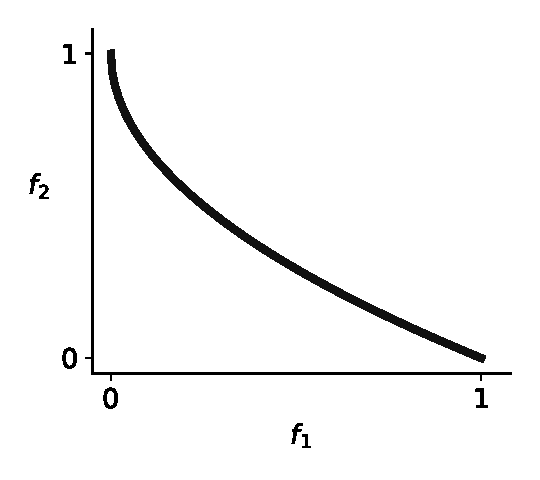
\includegraphics[height=0.33\textheight]{zdt1_frente.pdf}\\[-2mm]
      {\scriptsize $\ZdtF$\\[1mm] $\ZdtG$\\[0.5mm] \phantom{$\ZdtG$}}
    \end{column}
    \begin{column}{0.49\textwidth}
      \centering
      {\large\textbf{\DtlzName}} \quad \cita{\DtlzSize}\\[1mm]
      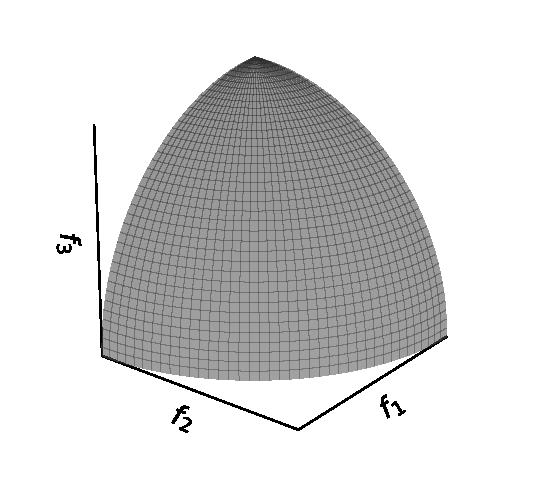
\includegraphics[height=0.33\textheight]{dtlz2_frente.pdf}\\[-2mm]
      {\scriptsize $\DtlzFone$\\[0.5mm] $\DtlzFtwo$\\[0.5mm] $\DtlzFthree$\\[1mm] $\DtlzG$}
    \end{column}
  \end{columns}
  \vspace{1mm}
  \begin{center}
    {\scriptsize Y a cada objetivo, su banda: \quad
    $\ZdtR$ \quad y \quad $\DtlzR$,\\[1mm]
    con $\marca{x_d}$ una variable que no está en el centro
    \cita{($\ZdtDrivers$ y $\DtlzDrivers$)} --- la regla de antes.}
  \end{center}
  \NotaIX
\end{frame}

% ---------------------------------------------------------------- 10
\begin{frame}{En p2: lo que te daba un orden, desaparece con el otro}
  \begin{columns}[c,onlytextwidth]
    \begin{column}{0.30\textwidth}
      \centering
      \begin{tikzpicture}[font=\tiny,scale=0.85,
          caja/.style={draw,rounded corners,minimum height=5mm,minimum width=18mm,align=center},
          filtro/.style={draw,rounded corners,minimum height=5mm,minimum width=13mm,align=center,thick},
          node distance=2.5mm and 4mm]
        \node[caja] (sample) {5000 puntos\\al azar};
        \node[caja,below=of sample] (eval) {una sola\\evaluación};
        \node[filtro,draw=phils,below=9mm of eval,xshift=4mm] (fls) {\pls};
        \node[filtro,draw=philu,below=of fls] (flu) {\plu};
        \node[filtro,draw=phicw,below=of flu] (fcw) {\pcw};
        \draw[-{Stealth}] (sample) -- (eval);
        % un carril a la izquierda, para que ninguna flecha cruce un cuadro
        \coordinate (lane) at ([xshift=-5mm]fls.west);
        \draw (eval.south) -- ++(0,-3mm) -| (lane);
        \draw (lane) -- (lane|-fcw.west);
        \draw[-{Stealth}] (lane|-fls.west) -- (fls.west);
        \draw[-{Stealth}] (lane|-flu.west) -- (flu.west);
        \draw[-{Stealth}] (lane|-fcw.west) -- (fcw.west);
        \node[below=3mm of fcw,align=center,gris,xshift=-2mm] {la misma lista, filtrada tres veces:\\lo único que cambia es el orden};
      \end{tikzpicture}
    \end{column}
    \begin{column}{0.68\textwidth}
      \centering
      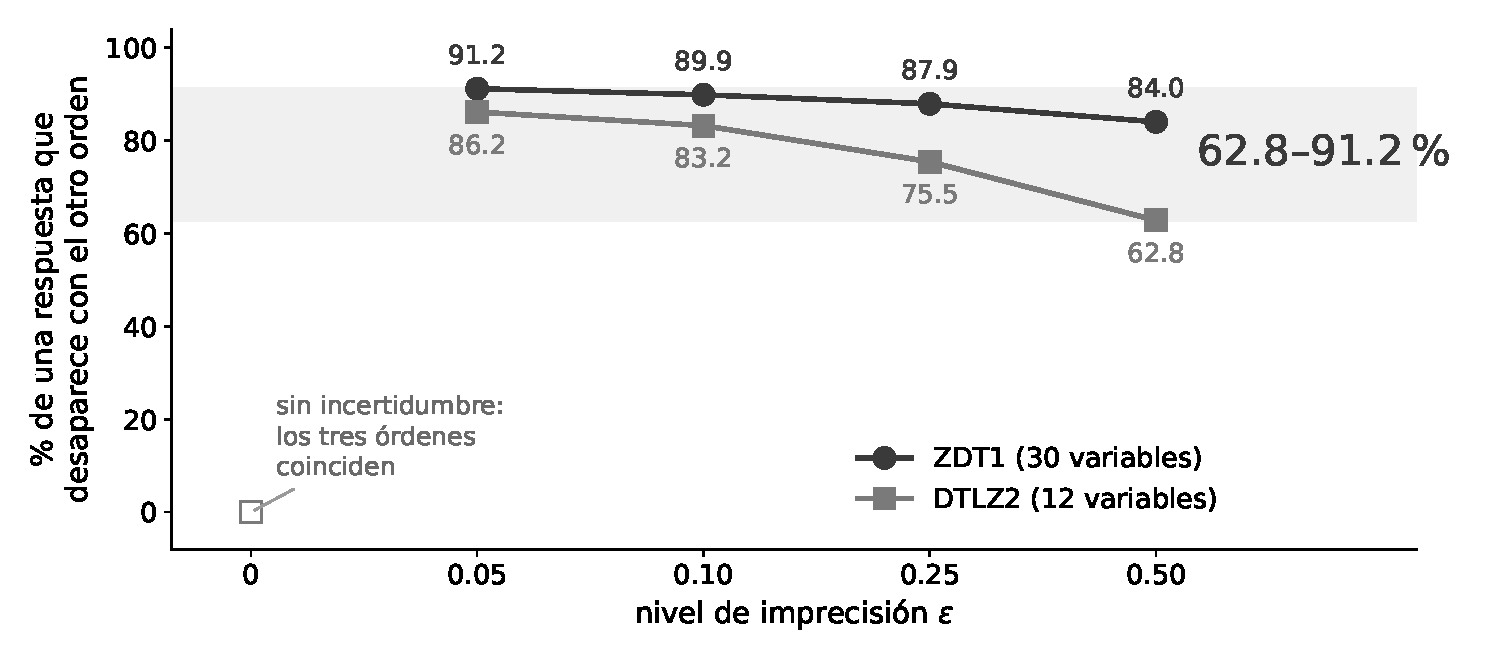
\includegraphics[width=0.98\textwidth,height=0.62\textheight,keepaspectratio]{benchmarks.pdf}
    \end{column}
  \end{columns}
  {\footnotesize Y como sé que mi medida dice que se parecen más de lo que se parecen, esto es un \textbf{mínimo}:
  \\ La diferencia real es mayor.}
  \NotaX
\end{frame}

% ---------------------------------------------------------------- 11
\begin{frame}{Y el tercero no lo he construido yo: está publicado}
  \centering
  \vspace{-2mm}
  {\footnotesize $\IBKone$,\quad $\IBKtwo$,\quad $x\in\IBKbox$}

  \vspace{-1mm}
  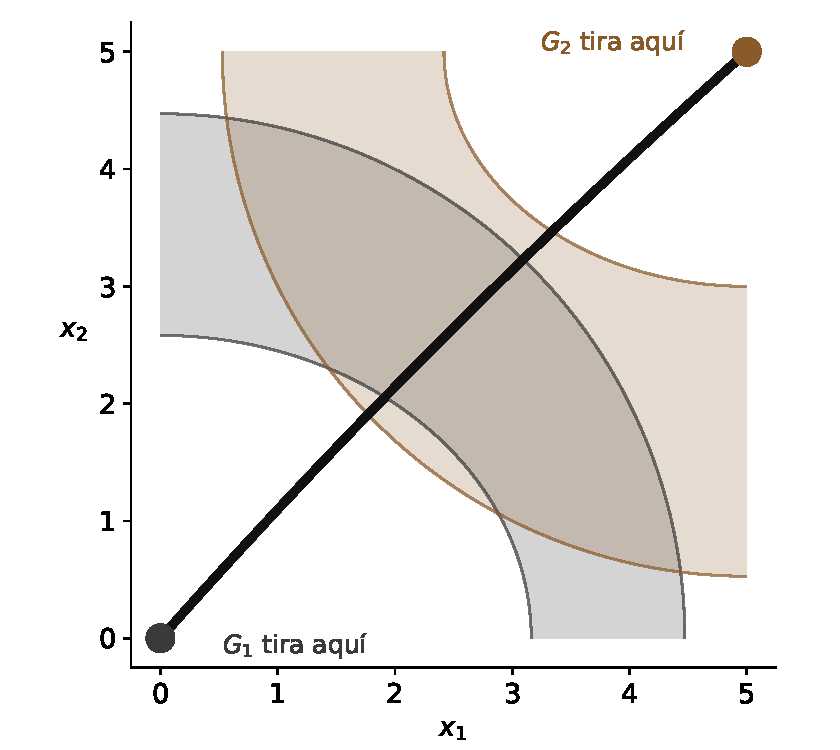
\includegraphics[height=0.69\textheight,keepaspectratio]{ibk1_crisp.pdf}

  \vspace{-1mm}
  {\footnotesize Cada objetivo vale un intervalo.}
  \NotaXI
\end{frame}

% ---------------------------------------------------------------- 12
\begin{frame}{Tres órdenes, tres respuestas: otra vez, y sin tocar el problema}
  \centering
  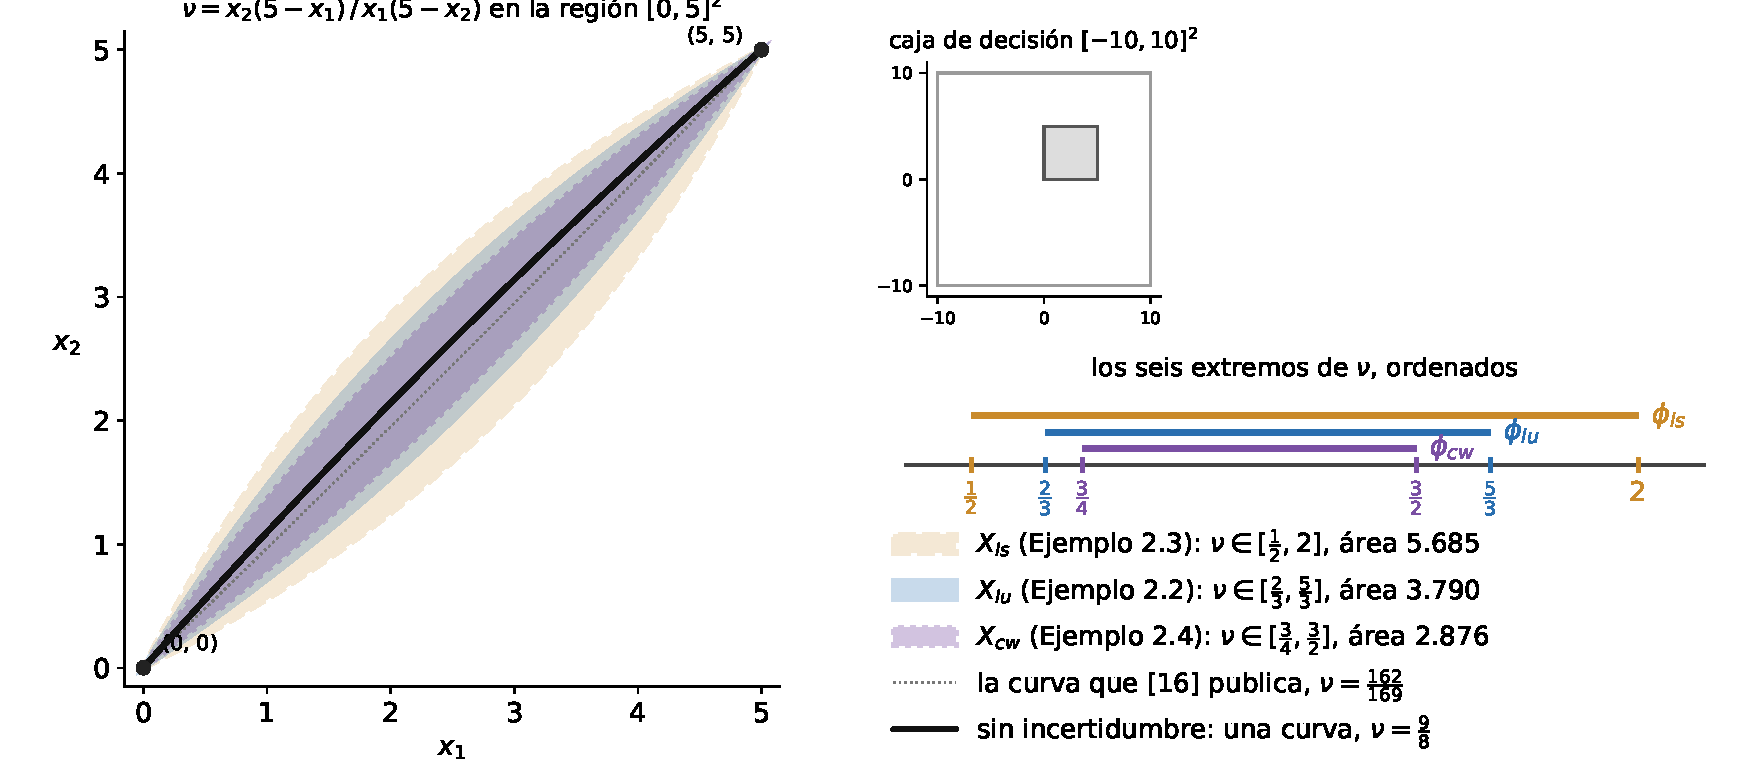
\includegraphics[width=0.98\textwidth,height=0.63\textheight,keepaspectratio]{ibk1_cunas.pdf}

  \vspace{-2mm}
  {\footnotesize Aquí las tres se meten una dentro de otra en vez de cruzarse: el
  \bMinInt--\bMaxInt\,\% de antes no vale aquí.\\ Lo que sí es
  exacto: el \textbf{\iLsOutsideCw\,\%} de la mayor queda fuera de la menor.}
  \NotaXII
\end{frame}

% ---------------------------------------------------------------- 13
\begin{frame}{Y de paso: el punto que publican como óptimo no lo es}
  \centering
  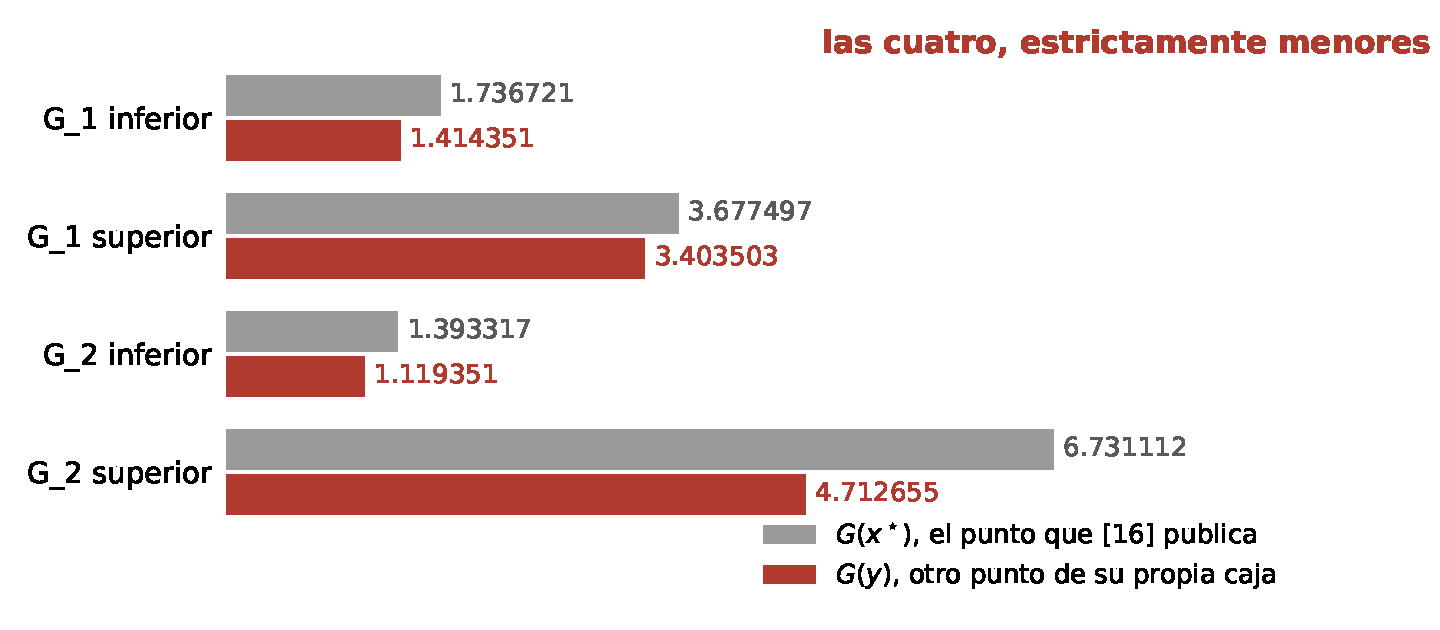
\includegraphics[width=0.88\textwidth,height=0.70\textheight,keepaspectratio]{contraejemplo.pdf}

  \vspace{-1mm}
  {\small Los de arriba son sus números; los de abajo salen con una calculadora
  en dos minutos.\\ \cita{Y los tres algoritmos lo encuentran.}}
  \NotaXIII
\end{frame}

% ---------------------------------------------------------------- cierre
\begin{frame}{Conclusiones}
  \vspace{4mm}
  \begin{center}
    \begin{minipage}{0.88\textwidth}
      {\large Elegir el orden no es un detalle de cómo montas el problema:\\
      \textbf{si no que condiciona la respuesta}.}
    \end{minipage}
  \end{center}
  \vspace{8mm}
  \begin{columns}[T,onlytextwidth]
    \begin{column}{0.32\textwidth}
      \centering
      {\LARGE\textbf{\pUnionShare\,\%}}\\[3mm]
      {\small es todo lo que dos órdenes\\ tienen en común}\\[2mm]
    \end{column}
    \begin{column}{0.32\textwidth}
      \centering
      {\LARGE\textbf{\bMinInt--\bMaxInt\,\%}}\\[3mm]
      {\small de tu respuesta desaparece\\ si te pasas al otro orden}\\[2mm]
    \end{column}
    \begin{column}{0.32\textwidth}
      \centering
      {\LARGE\textbf{\iLsOutsideCw\,\%}}\\[3mm]
      {\small de la respuesta mayor\\ se queda fuera de la menor}\\[2mm]
    \end{column}
  \end{columns}
  \vspace{7mm}
  \begin{center}
    \cita{Y siempre depende del problema: cada cifra viene de un problema concreto.}
  \end{center}
  \NotaXIV
\end{frame}

% ---------------------------------------------------------------- líneas futuras
\begin{frame}{Líneas futuras}
  \vspace{10mm}
  \begin{center}
    \begin{minipage}{0.82\textwidth}
      {\large
      \textbf{La curva de sensibilidad}: ir pasando poco a poco de un orden a
      otro, y ver cómo se mueve la respuesta.\\[8mm]
      \textbf{La aplicación a optimización de carteras}}
    \end{minipage}
  \end{center}
  \NotaXV
\end{frame}

\begin{frame}[plain]
  \vspace{10mm}
  \begin{center}
    {\Huge Gracias}\\[10mm]
  \end{center}
\end{frame}
\end{document}"
%                                                               -> presentacion_notas.pdf
\documentclass[aspectratio=169,11pt]{beamer}

\usetheme[numbering=fraction,progressbar=none,block=fill,background=light]{metropolis}
\usepackage[spanish,es-noshorthands,es-nodecimaldot]{babel}
\usepackage{amsmath,amssymb}
\usepackage{booktabs}
\usepackage{array}
\usepackage{tikz}
\usetikzlibrary{arrows.meta,positioning,calc,patterns,decorations.pathreplacing,shapes.geometric}
\usepackage{pgfpages}
\usepackage{appendixnumberbeamer}

% notas del orador: activadas con \def\shownotes{1} antes de \input
\ifdefined\shownotes
  \setbeameroption{show notes on second screen=right}
  \setbeamertemplate{note page}[plain]
  \setbeamerfont{note page}{size=\scriptsize}
\fi

% ---------------------------------------------------------------- colores
% Los tres órdenes llevan el mismo color en toda la presentación, y son los mismos
% tres valores hexadecimales que experiments/make_presentation.py usa en las
% figuras. Ninguno se lee como bueno o malo. La intersección se raya, nunca lleva
% un cuarto color.
\definecolor{philu}{HTML}{2A6FB0}
\definecolor{phils}{HTML}{C98A2B}
\definecolor{phicw}{HTML}{7A4FA3}
\definecolor{coefcol}{HTML}{B03A2E}
\definecolor{gris}{HTML}{6A6A6A}
\definecolor{grisclaro}{HTML}{DDDDDD}
\setbeamercolor{alerted text}{fg=coefcol}
\setbeamerfont{title}{size=\Large}

\newcommand{\plu}{\textcolor{philu}{$\phi_{lu}$}}
\newcommand{\pls}{\textcolor{phils}{$\phi_{ls}$}}
\newcommand{\pcw}{\textcolor{phicw}{$\phi_{cw}$}}
\newcommand{\Xlu}{\textcolor{philu}{$X_{lu}$}}
\newcommand{\Xls}{\textcolor{phils}{$X_{ls}$}}
\newcommand{\Xcw}{\textcolor{phicw}{$X_{cw}$}}
\newcommand{\coef}[1]{\textcolor{coefcol}{\boldsymbol{#1}}}
\newcommand{\marca}[1]{\textcolor{coefcol}{\boldsymbol{#1}}}
\newcommand{\cita}[1]{\textcolor{gris}{\small #1}}
\newcommand{\refuno}{[1] Costa, Osuna-Gómez y Chalco-Cano (2024)}
\newcommand{\refdieciseis}{[16] Mondal, Ghosh y Kim (2026)}

% ---------------------------------------------------------------- números generados
\graphicspath{{../results/figures/presentation/}}
% generated by experiments/make_presentation.py; do not edit.
% one \newcommand per number, each with the file and key it was read from.
% pRho: src/problems_tier0.py p1_default_params rho
\newcommand{\pRho}{\tfrac{1}{4}}
% pOffset: src/problems_tier0.py p1_default_params, the constant term of the half-width
\newcommand{\pOffset}{\tfrac{1}{8}}
% pBoxLo: src/problems_tier0.py p1_lower
\newcommand{\pBoxLo}{-\tfrac{1}{2}}
% pBoxHi: src/problems_tier0.py p1_upper
\newcommand{\pBoxHi}{\tfrac{3}{2}}
% pAreaLu: results/tier0/exact_regions_p1.csv area,lu
\newcommand{\pAreaLu}{0.311}
% pAreaLs: results/tier0/exact_regions_p1.csv area,ls
\newcommand{\pAreaLs}{1.513}
% pAreaCw: results/tier0/exact_regions_p1.csv area,cw
\newcommand{\pAreaCw}{1.000}
% pUnionShare: results/tier0/exact_regions_p1.csv overlap_union_share,lu,cw (in %)
\newcommand{\pUnionShare}{10.3}
% pLuOutsideCw: results/tier0/exact_regions_p1.csv 1 - coverage_a_in_b,lu,cw (in %)
\newcommand{\pLuOutsideCw}{60.5}
% pCwOutsideLu: results/tier0/exact_regions_p1.csv 1 - coverage_b_in_a,lu,cw (in %)
\newcommand{\pCwOutsideLu}{87.7}
% pCovLuCwExact: results/tier0/exact_regions_p1.csv coverage_a_in_b,lu,cw
\newcommand{\pCovLuCwExact}{0.395}
% pCovCwLuExact: results/tier0/exact_regions_p1.csv coverage_b_in_a,lu,cw
\newcommand{\pCovCwLuExact}{0.123}
% pJacExact: results/tier0/exact_regions_p1.csv overlap_union_share,lu,cw
\newcommand{\pJacExact}{0.103}
% pCovLuCwMeas: results/tier0/instrument_error_p1.csv (lu,cw; delta 0.0; n_evals 5000) measured_median, metric coverage_a_in_b
\newcommand{\pCovLuCwMeas}{0.556}
% pCovLuCwErr: results/tier0/instrument_error_p1.csv (lu,cw; delta 0.0; n_evals 5000) measured/exact, metric coverage_a_in_b
\newcommand{\pCovLuCwErr}{+40.8\,\%}
% pCovLuCwErrLarge: results/tier0/table_2_measured.csv decision block (lu,cw; delta 0.0; n_evals 20000) median/exact, metric coverage_a_in_b
\newcommand{\pCovLuCwErrLarge}{+27.7\,\%}
% pCovCwLuMeas: results/tier0/instrument_error_p1.csv (lu,cw; delta 0.0; n_evals 5000) measured_median, metric coverage_b_in_a
\newcommand{\pCovCwLuMeas}{0.222}
% pCovCwLuErr: results/tier0/instrument_error_p1.csv (lu,cw; delta 0.0; n_evals 5000) measured/exact, metric coverage_b_in_a
\newcommand{\pCovCwLuErr}{+81.0\,\%}
% pCovCwLuErrLarge: results/tier0/table_2_measured.csv decision block (lu,cw; delta 0.0; n_evals 20000) median/exact, metric coverage_b_in_a
\newcommand{\pCovCwLuErrLarge}{+48.6\,\%}
% pJacMeas: results/tier0/instrument_error_p1.csv (lu,cw; delta 0.0; n_evals 5000) measured_median, metric overlap via jaccard = dice/(2-dice)
\newcommand{\pJacMeas}{0.187}
% pJacErr: results/tier0/instrument_error_p1.csv (lu,cw; delta 0.0; n_evals 5000) measured/exact, metric overlap
\newcommand{\pJacErr}{$\times$1.81}
% pJacErrLarge: results/tier0/table_2_measured.csv decision block (lu,cw; delta 0.0; n_evals 20000) median/exact, metric overlap
\newcommand{\pJacErrLarge}{$\times$1.49}
% pJacFactorPlain: results/tier0/instrument_error_p1.csv (lu,cw; delta 0.0; n_evals 5000) jaccard measured/exact
\newcommand{\pJacFactorPlain}{1.81}
% pJacFactorLargePlain: results/tier0/table_2_measured.csv decision block (lu,cw; delta 0.0; n_evals 20000) jaccard measured/exact
\newcommand{\pJacFactorLargePlain}{1.49}
% bMinPct: results/tier1/table_2_measured_eps_{0.05,0.1,0.25,0.5}.csv decision block, lu,cw, finding, coverage_b_in_a, n_evals 5000, delta 0.0: min over the eight cells of 1 - median (in %)
\newcommand{\bMinPct}{62.8}
% bMaxPct: results/tier1/table_2_measured_eps_{0.05,0.1,0.25,0.5}.csv decision block, lu,cw, finding, coverage_b_in_a, n_evals 5000, delta 0.0: max over the eight cells of 1 - median (in %)
\newcommand{\bMaxPct}{91.2}
% bMinInt: results/tier1/table_2_measured_eps_{0.05,0.1,0.25,0.5}.csv decision block, lu,cw, finding, coverage_b_in_a, n_evals 5000, delta 0.0: min, rounded to the integer
\newcommand{\bMinInt}{63}
% bMaxInt: results/tier1/table_2_measured_eps_{0.05,0.1,0.25,0.5}.csv decision block, lu,cw, finding, coverage_b_in_a, n_evals 5000, delta 0.0: max, rounded to the integer
\newcommand{\bMaxInt}{91}
% bZdtVars: src/problems_tier1.py zdt1_n_vars
\newcommand{\bZdtVars}{30}
% bDtlzVars: src/problems_tier1.py dtlz2_n_vars
\newcommand{\bDtlzVars}{12}
% cZdtCardCw: results/tier1/table_2_measured_eps_{0.05,0.1,0.25,0.5}.csv decision block, lu,cw, finding, coverage_b_in_a, n_evals 5000, delta 0.0: cardinality_b, constant over the four eps
\newcommand{\cZdtCardCw}{257}
% cZdtCardLu: results/tier1/table_2_measured_eps_{0.05,0.1,0.25,0.5}.csv decision block, lu,cw, finding, coverage_b_in_a, n_evals 5000, delta 0.0: cardinality_a over eps 0.05, 0.1, 0.25, 0.5
\newcommand{\cZdtCardLu}{26\,\to\,36\,\to\,53\,\to\,68}
% cDtlzCardCw: results/tier1/table_2_measured_eps_{0.05,0.1,0.25,0.5}.csv decision block, lu,cw, finding, coverage_b_in_a, n_evals 5000, delta 0.0: cardinality_b, constant over the four eps
\newcommand{\cDtlzCardCw}{1813}
% cDtlzCardLu: results/tier1/table_2_measured_eps_{0.05,0.1,0.25,0.5}.csv decision block, lu,cw, finding, coverage_b_in_a, n_evals 5000, delta 0.0: cardinality_a over eps 0.05, 0.1, 0.25, 0.5
\newcommand{\cDtlzCardLu}{278\,\to\,351\,\to\,575\,\to\,980}
% ZdtName: src/problems_tier1.py zdt1_interval
\newcommand{\ZdtName}{ZDT1}
% ZdtSize: src/problems_tier1.py zdt1_n_vars, zdt1_n_obj
\newcommand{\ZdtSize}{30 variables, 2 objetivos}
% ZdtF: src/problems_tier1.py evaluate_zdt1, [2] equations (6) and (7)
\newcommand{\ZdtF}{f_1 = x_1, \qquad f_2 = g\,\Bigl(1 - \sqrt{f_1/g}\,\Bigr)}
% ZdtG: src/problems_tier1.py evaluate_zdt1, g with m - 1 = zdt1_n_vars - 1
\newcommand{\ZdtG}{g = 1 + \dfrac{9}{29}\sum_{i \geq 2} x_i}
% ZdtR: src/problems_tier1.py zdt1_half_width
\newcommand{\ZdtR}{r_i = \varepsilon\,\bigl( (\marca{x_d} - \tfrac{1}{2})^2 + \tfrac{1}{20} \bigr)}
% ZdtDrivers: src/problems_tier1.py zdt1_width_drivers, as 1-based names
\newcommand{\ZdtDrivers}{x_{30}, x_{29}}
% DtlzName: src/problems_tier1.py dtlz2_interval
\newcommand{\DtlzName}{DTLZ2}
% DtlzSize: src/problems_tier1.py dtlz2_n_vars, dtlz2_n_obj
\newcommand{\DtlzSize}{12 variables, 3 objetivos}
% DtlzFone: src/problems_tier1.py evaluate_dtlz2, [3] equation (9) at M = 3
\newcommand{\DtlzFone}{f_1 = (1+g)\cos\tfrac{\pi x_1}{2}\cos\tfrac{\pi x_2}{2}}
% DtlzFtwo: src/problems_tier1.py evaluate_dtlz2, [3] equation (9) at M = 3
\newcommand{\DtlzFtwo}{f_2 = (1+g)\cos\tfrac{\pi x_1}{2}\sin\tfrac{\pi x_2}{2}}
% DtlzFthree: src/problems_tier1.py evaluate_dtlz2, [3] equation (9) at M = 3
\newcommand{\DtlzFthree}{f_3 = (1+g)\sin\tfrac{\pi x_1}{2}}
% DtlzG: src/problems_tier1.py evaluate_dtlz2, g over the tail
\newcommand{\DtlzG}{g = \sum_{i \geq 3} (x_i - \tfrac{1}{2})^2}
% DtlzR: src/problems_tier1.py dtlz2_half_width
\newcommand{\DtlzR}{r_i = \varepsilon\,\marca{x_d}}
% DtlzDrivers: src/problems_tier1.py dtlz2_width_drivers, as 1-based names
\newcommand{\DtlzDrivers}{x_{12}, x_{11}, x_{10}}
% IBKone: src/problems_native.py ibk1_coefficients[0]
\newcommand{\IBKone}{G_1 = \coef{[0.1, 0.2]}\, x_1^2 + \coef{[0.1, 0.3]}\, x_2^2}
% IBKtwo: src/problems_native.py ibk1_coefficients[1], ibk1_shift
\newcommand{\IBKtwo}{G_2 = \coef{[0.1, 0.3]}\, (x_1 - 5)^2 + \coef{[0.1, 0.5]}\, (x_2 - 5)^2}
% IBKbox: src/problems_native.py ibk1_lower, ibk1_upper
\newcommand{\IBKbox}{[-10, 10]^2}
% IBKratiosOne: computed from ibk1_coefficients[0]: (b-a)/(a+b) per term
\newcommand{\IBKratiosOne}{\tfrac{1}{3} frente a \tfrac{1}{2}}
% IBKratiosTwo: computed from ibk1_coefficients[1]: (b-a)/(a+b) per term
\newcommand{\IBKratiosTwo}{\tfrac{1}{2} frente a \tfrac{2}{3}}
% iAreaLu: results/part2/exact_regions_ibk1.csv area,lu
\newcommand{\iAreaLu}{3.790}
% iBandLuLo: results/part2/exact_regions_ibk1.csv band_lower,lu
\newcommand{\iBandLuLo}{\tfrac{2}{3}}
% iBandLuHi: results/part2/exact_regions_ibk1.csv band_upper,lu
\newcommand{\iBandLuHi}{\tfrac{5}{3}}
% iAreaLs: results/part2/exact_regions_ibk1.csv area,ls
\newcommand{\iAreaLs}{5.685}
% iBandLsLo: results/part2/exact_regions_ibk1.csv band_lower,ls
\newcommand{\iBandLsLo}{\tfrac{1}{2}}
% iBandLsHi: results/part2/exact_regions_ibk1.csv band_upper,ls
\newcommand{\iBandLsHi}{2}
% iAreaCw: results/part2/exact_regions_ibk1.csv area,cw
\newcommand{\iAreaCw}{2.876}
% iBandCwLo: results/part2/exact_regions_ibk1.csv band_lower,cw
\newcommand{\iBandCwLo}{\tfrac{3}{4}}
% iBandCwHi: results/part2/exact_regions_ibk1.csv band_upper,cw
\newcommand{\iBandCwHi}{\tfrac{3}{2}}
% iOrderedEnds: results/part2/exact_regions_ibk1.csv the six band ends, sorted
\newcommand{\iOrderedEnds}{\tfrac{1}{2} < \tfrac{2}{3} < \tfrac{3}{4} < \tfrac{3}{2} < \tfrac{5}{3} < 2}
% iLsOutsideCw: results/part2/exact_regions_ibk1.csv 1 - coverage_a_in_b,ls,cw (in %)
\newcommand{\iLsOutsideCw}{49.4}
% iCovLsCw: results/part2/exact_regions_ibk1.csv coverage_a_in_b,ls,cw
\newcommand{\iCovLsCw}{0.506}
% iNuCurve: docs/part2/f2_ibk1_derivation.md section 4.1, nu of equation (25)'s curve
\newcommand{\iNuCurve}{\tfrac{162}{169}}
% iCritRatio: docs/part2/f2_ibk1_derivation.md section 4.3, critical set measure over X_lu's
\newcommand{\iCritRatio}{4.24}
% iNuCrisp: computed from src/problems_native.py's coefficients and checked against docs/part2/f2_ibk1_derivation.md section 3.3
\newcommand{\iNuCrisp}{\tfrac{9}{8}}
% IVUone: [16] appendix A problem 2, as docs/part2/f7_ivu2_derivation.md transcribes it
\newcommand{\IVUone}{G_1 = \coef{[1, 1.5]}\, \marca{x_1} + \coef{[1, 1.5]}\, \marca{x_2} + \coef{[1, 1]}}
% IVUtwo: [16] appendix A problem 2, as docs/part2/f7_ivu2_derivation.md transcribes it
\newcommand{\IVUtwo}{G_2 = \coef{[1, 1.5]}\, x_1^2 + \coef{[2, 3]}\, x_2^2 - \coef{[1, 1]}}
% IVUbox: [16] appendix A problem 2, as docs/part2/f7_ivu2_derivation.md transcribes it
\newcommand{\IVUbox}{[-4, 4]^2}
% dXstar: [16] Table 1 page 20, as docs/part2/f2_ibk1_derivation.md section 4.2 (re-computed here in exact rationals from src/problems_native.py's coefficients and asserted equal)
\newcommand{\dXstar}{(3.914930, 1.428474)}
% dY: docs/part2/f2_ibk1_derivation.md section 4.2 (re-computed here in exact rationals from src/problems_native.py's coefficients and asserted equal)
\newcommand{\dY}{(2.8975, 2.3975)}
% dMinMargin: docs/part2/f2_ibk1_derivation.md section 4.2 (re-computed here in exact rationals from src/problems_native.py's coefficients and asserted equal): the smallest of the four margins
\newcommand{\dMinMargin}{0.274}
% dConfigs: results/part2/dominators_summary.csv: number of rows (solver x phi x budget)
\newcommand{\dConfigs}{18}
% dConfigsWithDominator: results/part2/dominators_summary.csv: rows with seeds_with_a_dominator == n_seeds
\newcommand{\dConfigsWithDominator}{18}
% dWidestMargin: results/part2/dominators_summary.csv: max of widest_margin_over_seeds
\newcommand{\dWidestMargin}{0.270}
% iJacFactorMin: results/part2/instrument_error_ibk1.csv, metric overlap, delta 0.0, jaccard = dice/(2-dice), measured/exact over the three pairs (min)
\newcommand{\iJacFactorMin}{1.01}
% iJacFactorMax: results/part2/instrument_error_ibk1.csv, metric overlap, delta 0.0, jaccard = dice/(2-dice), measured/exact over the three pairs (max)
\newcommand{\iJacFactorMax}{1.48}
% aCorrProportional: docs/part1/a1_uncertainty_model.md part 1, the proportional width, corr(centre, width)
\newcommand{\aCorrProportional}{+1.0000}
% rWidthValuesTrue: docs/explicacion_proyecto.md section 10.3
\newcommand{\rWidthValuesTrue}{46}
% rWidthValuesSeen: docs/explicacion_proyecto.md section 10.3
\newcommand{\rWidthValuesSeen}{210}
% rGridPoints: docs/explicacion_proyecto.md section 10.5
\newcommand{\rGridPoints}{40401}
% rFixedCoverage: instrument_error_p1.csv, instrument_error_ibk1.csv, table_2_measured_eps_*.csv: every check row with a containment-fixed direction
\newcommand{\rFixedCoverage}{1.000000}
% rFixedRange: same rows: q3 - q1
\newcommand{\rFixedRange}{0}
% rFixedRows: same rows: how many were checked
\newcommand{\rFixedRows}{28}
% rSatConfigs: results/tier1/rank_one_summary.csv: nsga2 rows with eps > 0 at n_evals 5000
\newcommand{\rSatConfigs}{24}
% rGenerations: results/tier1/rank_one_summary.csv: n_generations
\newcommand{\rGenerations}{50}

% generated by experiments/make_presentation.py from presentation/guion.txt
% one command per slide, in order; presentacion.tex uses them inside \note{}.
\newcommand{\NotaI}{\note{Optimizar es buscar el mejor valor de algo. Con un objetivo hay una respuesta: un punto. En la práctica casi nunca hay uno solo: quieres bajar el coste y bajar el riesgo, y se contradicen. Como optimizar un programa para que sea rápido y gaste poca memoria: no existe el mejor programa. Cuando hay varios objetivos ya no hay un ganador único: hay un conjunto de soluciones que no se pueden mejorar en un objetivo sin empeorar otro. Se llama conjunto eficiente, o frente de Pareto. La regla que lo define es la dominancia, la de la caja. Esto es todo lo que hace falta saber de optimización multiobjetivo}}
\newcommand{\NotaII}{\note{En la realidad no sabemos los valores exactos de las variables. El coste no es 40, es entre 38 y 45: hay un error de medida, hay parámetros que varían, información incompleta. Un intervalo es eso. Tres palabras que hay que fijar ya: centro, semianchura y anchura. Y los objetivos ahora son intervalos, dejan de poder ordenarse. Con A=(1’5 , 5) y =(3,7’5) A parece menor. Pero con A igual a uno a diez y B igual a cuatro a cinco, A puede ser mejor o mucho peor. No hay respuesta. No es un problema técnico: es que no existe una única forma correcta de ordenar intervalos. Existen muchas, y cada una es una decisión sobre qué te importa.}}
\newcommand{\NotaIII}{\note{El primer artículo de Rafaela … , hizo algo elegante: en vez de proponer un orden, describió toda la familia de órdenes posibles, con un parámetro que dice cuál estás usando. Ese parámetro es fi. Un fi coge un intervalo y devuelve dos números reales, que sí se pueden comparar. Los tres que el artículo nombra: fi\_Lu, compara mejor caso con mejor caso y peor con peor fi\_Ls, extremo inferior y anchura; fi\_cw, centro y semianchura. Los tres son válidos, distintos, y cada uno da un conjunto eficiente distinto. Analogía: fi es la función clave de un sort. La regla: m objetivos intervalares se convierten en dos m objetivos reales, y eso ya se sabe resolver con NSGA-II o PSO. El artículo demuestra que resolver el transformado equivale a resolver el original}}
\newcommand{\NotaIV}{\note{Y con esto ya puedo decir qué es lo que me pregunto, que es una sola cosa: si cambio el orden y no cambio nada más, ¿cambia la respuesta? ¿Y cuánto? Hay otra pregunta que la gente hace enseguida y que yo no contesto: cuál de los tres órdenes es el bueno. No la contesto porque no se puede con lo que tengo delante. Cada orden mira el problema a su manera, y para decir cuál acierta haría falta saber qué pasa de verdad después, en la realidad. Estos problemas de prueba no lo dicen. Prefiero decirlo yo ahora y no que se quede la duda.}}
\newcommand{\NotaV}{\note{Lo primero que hice fue lo obvio, y salió mal. Es el hallazgo del que más he aprendido. Cogí un problema normal y le puse un margen de error fijo arriba y abajo: en vez de un número, un intervalo de ancho siempre igual. Parece sensato y es inútil. Si todos los intervalos tienen el mismo ancho, dos de los tres órdenes están mirando un número que nunca cambia. Y un dato que es siempre el mismo no sirve para ordenar nada: es como ordenar una lista de gente por el número siete. Resultado: los tres órdenes daban exactamente el mismo conjunto, y encima el mismo que si no hubiera incertidumbre. Y no lo deduje, lo medí: los tres conjuntos salieron con los mismos puntos, uno por uno. De aquí sale la regla que gobierna todo lo demás: la incertidumbre tiene que depender de algo que el valor central no controle. Si el ancho se puede calcular a partir del centro, los tres órdenes se vuelven el mismo. Si hubiera montado el estudio sin darme cuenta de esto, todas mis tablas habrían salido llenas de unos y habría concluido que el orden da igual. Que es justo lo contrario de la verdad.}}
\newcommand{\NotaVI}{\note{Antes de enseñaros lo que sale, un minuto con el problema, porque si no la siguiente imagen no se entiende. Me construí un problema de dos variables, a medida, para poder resolverlo a mano. Los dos objetivos son lo mismo: acércate a un punto. Uno te pide acercarte a éste y el otro a éste de aquí. Si sólo tuviera el primero, la respuesta sería ese punto, y ya está. Si sólo tuviera el segundo, el otro. Pero no puedo estar en los dos sitios a la vez. Y fijaos en lo que pasa con cualquier punto que no esté en la línea: si tiro hacia la línea me acerco a los dos objetivos a la vez, así que ese punto no puede ser una respuesta, porque hay otro mejor en todo. Conclusión: sin incertidumbre, la respuesta de este problema es exactamente el segmento que une los dos puntos. Una línea. Quedaos con esa línea, porque ahora le voy a meter la incertidumbre y vamos a ver qué le pasa.}}
\newcommand{\NotaVII}{\note{Así que me construí un problema a medida, con dos variables, para poder resolverlo a mano. Tiene dos objetivos, y la gracia está en el cruce: la incertidumbre de cada objetivo depende de la variable del otro. Que es la regla de antes, aplicada. Y como todo es cuadrático, las condiciones de optimalidad se convierten en un sistema de ecuaciones que se resuelve con papel y lápiz. Usando el Teorema 3.3 y el Ejemplo 3.9 del artículo de Rafaela — sus propios resultados, aplicados, no inventados por mí — saco la respuesta exacta bajo cada uno de los tres órdenes. Y esto es lo que sale. Esto no es lo que me ha devuelto un ordenador: son las tres fórmulas dibujadas. No hay muestreo ni algoritmo dentro. Los dos ejes son las dos variables. El cuadrado es la respuesta con un orden, la región grande con otro, la lente con el tercero. Mismo problema, mismos datos; lo único que cambia es el orden. Y mirad lo que pasa: la lente y el cuadrado no se contienen. La lente sube por arriba, donde el cuadrado no llega; el cuadrado ocupa todo lo de abajo, donde la lente no llega. Cada uno tiene una zona a la que el otro no alcanza. De todo lo que podrían tener en común, sólo comparten el diez por ciento. Y esto es exacto, medido sobre las fórmulas. Si alguien está eligiendo entre soluciones, cambiar de orden le cambia casi toda la lista.}}
\newcommand{\NotaVIII}{\note{Ahora, en un problema así yo tengo la respuesta exacta. Pero en un problema de verdad no la voy a tener: voy a tener lo que me devuelva el ordenador. Así que aproveché: tengo las dos cosas a la vez, lo exacto y lo medido, y las puse una al lado de la otra. Esto es algo que casi ningún trabajo tiene: sé cuánto se equivoca mi propio instrumento. Y se equivoca siempre en la misma dirección: dice que los dos órdenes se parecen más de lo que se parecen. Donde de verdad comparten un diez por ciento, él dice dieciocho. La razón es fácil de ver: cuando pruebas puntos al azar, encuentras primero los fáciles, y los fáciles son justo los que están en la zona común. Lo que pertenece a un solo conjunto está en los bordes y cuesta más pillarlo. Ese factor, casi el doble, es de este problema. No lo llevo a ningún otro sitio ni corrijo ningún número con él.}}
\newcommand{\NotaIX}{\note{Hasta aquí todo ha sido un problema de dos variables que me inventé yo. Toca salir a problemas de verdad. Éstos son dos de los que se usan como referencia en el campo: ZDT1 y DTLZ2. No son míos: están publicados y todo el mundo los conoce. El primero tiene treinta variables y dos objetivos, y su respuesta, sin incertidumbre, es esa curva. El segundo tiene doce variables y tres objetivos, y su respuesta es ese trozo de esfera. Fijaos en el salto: antes la respuesta era un segmento en un plano que cabía en una imagen; aquí ya no puedo dibujar el espacio de las soluciones, porque tiene treinta dimensiones. A los dos les pongo una banda de incertidumbre encima, con la regla del principio: la anchura la mueve una variable que no está en el centro. Está marcada en rojo. Y el parámetro épsilon es cuánta imprecisión les meto. Voy a probar cuatro niveles.}}
\newcommand{\NotaX}{\note{Aquí está el método, y es lo que hace que el número de la derecha valga algo. Va de arriba abajo, por el esquema de la izquierda. Uno: cojo cinco mil puntos al azar dentro de la caja. Al azar de verdad, sin mirar los objetivos y sin usar nada de lo que sé del problema. Dos: evalúo esos cinco mil puntos una sola vez. Cada punto me devuelve sus intervalos, uno por objetivo, y esa lista ya no se vuelve a tocar. Tres: cojo esa única lista y la filtro tres veces. En cada pasada uso uno de los tres órdenes: comparo los puntos entre sí con ese criterio y me quedo con los que no domina nadie. Tres pasadas sobre la misma lista, tres subconjuntos. Y aquí está la gracia: los tres salen de los mismos puntos y de los mismos números; lo único distinto es el criterio con el que comparo. Así que cualquier diferencia entre ellos es del orden y de nada más. Si lanzara un algoritmo evolutivo tres veces, una con cada orden, cambiaría dos cosas a la vez: el criterio, que es lo que quiero medir, y por dónde busca el algoritmo. Saldrían mezcladas y no podría separarlas. Por eso probar al azar no es el rival flojo: es el instrumento con el que mido. NSGA-II y el PSO multiobjetivo sí están en el trabajo, pero en otro sitio: comprobando que los solvers llegan a donde la derivación dice, y en la última diapositiva. Y esto es lo que sale: entre el sesenta y tres y el noventa y uno por ciento de lo que te daba un orden desaparece si te pasas al otro. Y como ya sé que mi instrumento exagera el parecido, esto es un mínimo: la diferencia real es mayor. No están inflados a mi favor, sino en mi contra. Abajo a la izquierda, la comprobación: sin incertidumbre, los tres órdenes vuelven a dar lo mismo.}}
\newcommand{\NotaXI}{\note{Llegados aquí alguien puede decirme, con toda la razón: claro, te has construido tú el problema para que salga lo que querías. Y es verdad, y por eso está medido y escrito. Así que el tercer problema no lo he tocado yo. Está publicado por otros autores, para otra cosa, antes de que yo empezara. Y es intervalar de origen: los intervalos están en los propios coeficientes, ahí arriba, entre corchetes. Yo no elegí ni cuánto valen ni de qué variable dependen. Por dentro es el mismo tipo de problema que el mío: dos objetivos, y cada uno te pide acercarte a una esquina. Uno tira hacia el cero y el otro hacia el cinco cinco. Con una diferencia que se ve en el dibujo: como los coeficientes son intervalos, un objetivo ya no vale un número. Pedirle que valga dos no te da una curva, te da esa banda sombreada. Y como antes: si quito la incertidumbre y me quedo con los valores centrales, la respuesta es una sola curva, la negra. Quedaos otra vez con esa curva.}}
\newcommand{\NotaXII}{\note{Y esto es lo que sale al derivarlo a mano, que es más bonito de lo que esperaba: toda la respuesta cabe en un solo número. Cada orden se queda con los puntos cuyo número cae dentro de un intervalo, y el intervalo depende del orden. Tres cuñas, ancladas en las mismas dos esquinas, con la curva de antes por el medio. Otra vez tres órdenes, tres respuestas distintas, en un problema que no es mío. Y fijaos en el salto: sin incertidumbre era una curva; con cada orden es una región con superficie. Pero aquí tengo que ser honesto con una cosa: estas tres se meten una dentro de otra, no se cruzan como antes. Así que el número del sesenta y tres al noventa y uno no tiene equivalente aquí, y no lo reclamo. Lo que sí puedo decir es que la mitad de la mayor se queda fuera de la menor. Y hay una comprobación que no es mía y que sale bien: ellos publican una curva de soluciones, la calculo, y cae dentro de las tres cuñas. Un apunte más, porque marca el límite: derivé un segundo problema suyo y ahí los tres órdenes dan exactamente lo mismo. O sea que ser un problema intervalar de verdad no basta para que el orden importe. Se sabe mirando los coeficientes, antes de resolver nada.}}
\newcommand{\NotaXIII}{\note{Y esto salió de paso. No me puse a buscar errores en nadie: me puse a comprobar mi propia derivación contra lo que ellos publican, que es lo que hay que hacer. Ellos dan este punto como solución óptima de su problema. Su propia definición dice qué significa eso: que no exista otro punto que sea igual o mejor en las cuatro cantidades. Cogí otro punto, que está dentro de su misma caja, y lo comparé con los números que ellos imprimen. Las cuatro salen menores. Las cuatro. Los de arriba son sus números, tal como están en el artículo; los de abajo se calculan con una calculadora en dos minutos. No hace falta creerse nada de lo que yo he hecho. Y no es cosa del redondeo: la diferencia más ajustada es doscientas mil veces mayor que lo que podría moverse el último decimal que ellos imprimen. Además, los tres algoritmos lo encuentran solos. A la sesión que los lanzó no se le dijo nada de este punto, y las dieciocho configuraciones devolvieron puntos que lo ganan. Es una corrección, no una crítica. Y lo que no digo es dónde está el fallo de su demostración: se apoya en otro artículo suyo que yo no tengo. Digo que la conclusión es falsa; no digo por qué.}}
\newcommand{\NotaXIV}{\note{Y resumo con lo que defiendo, que es una sola cosa: elegir el orden no es un detalle de cómo montas el problema, es media respuesta. Con tres medidas. En mi problema, hecho a mano y exacto: de todo lo que podrían tener en común dos órdenes, sólo comparten el diez por ciento. En dos problemas de referencia del campo, medido: entre el sesenta y tres y el noventa y uno por ciento de lo que te daba un orden desaparece si te pasas al otro. Y con un instrumento cuyo error conozco, así que eso es un mínimo. Y en un problema publicado por otros, que no he tocado yo: la mitad de la respuesta mayor se queda fuera de la menor. Todo esto bajo una condición sobre el modelo de incertidumbre que no supuse, sino que medí, y que además se puede comprobar en cualquier problema antes de ponerse a resolver. Y tres cosas que no sé, y que están escritas: por qué a uno de los algoritmos le cuesta más de lo que debería, después de descartar cinco explicaciones midiéndolas; por qué en un problema las respuestas se cruzan y en otro se anidan; y por qué mi instrumento se equivoca casi el doble en un problema y casi nada en otro. Que esas tres estén escritas es parte del resultado, no un defecto.}}
\newcommand{\NotaXV}{\note{Y lo que queda por hacer, que son dos cosas. La primera es la curva de sensibilidad: en vez de tres órdenes sueltos, ir pasando poco a poco de uno a otro y ver cómo se mueve la respuesta. Es admisible por la propia definición del artículo y el código está montado para que sea un bucle; fue lo primero que me quité de encima por falta de tiempo, y es la mejora más grande que hay disponible. Y la segunda son las carteras, que es donde vuestra propia propuesta las pone, como trabajo futuro. Gracias.}}


\title{Técnicas de Optimización Intervalar basadas en Inteligencia Computacional}
\subtitle{¿Cuánto cambia la respuesta cuando lo único que cambia es el orden?}
\author{Francisco Rodríguez-Carretero Roldán}
\institute{Tutores: Antonio Beato Moreno y Rafaela Osuna Gómez · Universidad de Sevilla}
\date{25 de septiembre de 2026 · Proyecto PI3, julio--septiembre 2026}

\begin{document}

% ================================================================ portada
\begin{frame}[plain]
  \vspace{-6mm}\titlepage
\end{frame}

% ================================================================ BLOQUE A
% ---------------------------------------------------------------- 1
\begin{frame}{Optimizar con varios objetivos: no hay un ganador, hay un conjunto}
  \begin{columns}[T]
    \begin{column}{0.52\textwidth}
      \centering
      \begin{tikzpicture}[scale=0.55]
        \draw[-{Stealth}] (0,0) -- (10.5,0) node[below left] {coste};
        \draw[-{Stealth}] (0,0) -- (0,9.5) node[below right,rotate=0] {riesgo};
        % dominados
        \foreach \x/\y in {3/7, 5/6, 6/4.5, 8/4, 4/6.5, 7/3.5, 9/5, 2.5/8.5, 5.5/8, 8.5/6.5, 3.5/5.5, 6.5/6}
          \fill[gris!60] (\x,\y) circle (0.14);
        % no dominados
        \draw[dashed,gris] plot[smooth] coordinates {(1,8) (2,5.5) (3.5,4) (5,3) (7,2.2) (9,1.8)};
        \foreach \x/\y in {1/8, 2/5.5, 3.5/4, 5/3, 7/2.2, 9/1.8}
          \fill[philu] (\x,\y) circle (0.2);
        \node[philu,align=left,font=\small] at (7.6,7.8) {conjunto eficiente\\(frente de Pareto)};
        \node[gris,font=\small] at (6.2,1.2) {dominados};
      \end{tikzpicture}
    \end{column}
    \begin{column}{0.46\textwidth}
      Bajar el coste sube el riesgo: no hay una solución única, existe un conjunto
      de soluciones eficientes.
      \begin{block}{Dominancia}
        $A$ domina a $B$ si $A$ es igual o mejor que $B$ en \textbf{todos} los
        objetivos y estrictamente mejor en \textbf{al menos uno}.
      \end{block}
      \vspace{2mm}
      Una solución es \textbf{eficiente} si nadie la domina.\\[2mm]
    \end{column}
  \end{columns}
  \NotaI
\end{frame}

% ---------------------------------------------------------------- 2
\begin{frame}{Bajo incertidumbre, los intervalos no siempre se ordenan intuitivamente}
  \centering
  \begin{tikzpicture}[scale=0.66]
    % el intervalo [38, 45]
    \begin{scope}
      \draw[thick] (0,0) -- (7,0);
      \draw[very thick,philu] (1,0) -- (6,0);
      \draw[very thick,philu] (1,-0.15) -- (1,0.15) node[above] {$38$};
      \draw[very thick,philu] (6,-0.15) -- (6,0.15) node[above] {$45$};
      \fill[philu] (3.5,0) circle (0.07) node[above,text=black] {centro $41.5$};
      \draw[decorate,decoration={brace,mirror,amplitude=4pt}] (1,-0.3) -- (3.5,-0.3)
        node[midway,below=4pt,font=\small,text=black] {semianchura $3.5$};
      \draw[decorate,decoration={brace,mirror,amplitude=4pt}] (1,-1.1) -- (6,-1.1)
        node[midway,below=4pt,font=\small,text=black] {anchura $7$};
      \node[right,font=\small,gris,align=left,text width=4.8cm] at (7.6,0.2) {``el coste no es $40$, es $[38, 45]$''};
    \end{scope}
    % A = [1.5, 5], B = [3, 7.5]
    \begin{scope}[yshift=-4.6cm]
      \draw[-{Stealth}] (0,0) -- (10,0) node[right] {$\mathbb{R}$};
      \foreach \x in {0,1,...,9} \draw (\x,-0.08) -- (\x,0.08) node[below=2pt,font=\scriptsize] {\x};
      \draw[very thick,philu] (1.5,0.5) -- (5,0.5) node[midway,above,font=\small] {$A = [1.5, 5]$};
      \draw[very thick,phicw] (3,1.5) -- (7.5,1.5) node[midway,above,font=\small] {$B = [3, 7.5]$};
      \node[right,font=\small,align=left,text width=4.8cm] at (10.6,0.9) {$A$ empieza y acaba antes:\\ aquí $A$ parece menor.};
    \end{scope}
    \begin{scope}[yshift=-8.2cm]
      \draw[-{Stealth}] (0,0) -- (10,0) node[right] {$\mathbb{R}$};
      \foreach \x in {0,1,...,9} \draw (\x,-0.08) -- (\x,0.08);
      \draw[very thick,philu] (1,0.5) -- (10,0.5) node[midway,above,font=\small] {$A = [1, 10]$};
      \draw[very thick,phicw] (4,1.5) -- (5,1.5) node[midway,above,font=\small] {$B = [4, 5]$};
      \node[right,font=\small,align=left,text width=4.8cm] at (10.6,0.9) {\textbf{¿Cuál es menor?}\\ No hay respuesta.};
    \end{scope}
  \end{tikzpicture}
  \NotaII
\end{frame}

% ---------------------------------------------------------------- 3
\begin{frame}{Una familia entera de órdenes, con un parámetro que dice cuál usas: $\phi$}
  \begin{columns}[c,onlytextwidth]
    \begin{column}{0.27\textwidth}
      \centering
      \begin{tikzpicture}[node distance=3.5mm,every node/.style={font=\small}]
        \node[draw,rounded corners,minimum height=7mm] (in) {$[\,l,\,u\,]$};
        \node[draw,rounded corners,fill=grisclaro,minimum height=7mm,right=of in] (phi) {$\phi$};
        \node[draw,rounded corners,minimum height=7mm,right=of phi] (out) {$(a,\,b)$};
        \draw[-{Stealth}] (in) -- (phi);
        \draw[-{Stealth}] (phi) -- (out);
      \end{tikzpicture}\\[1mm]
      {\small\color{gris} dos reales sí se comparan}
    \end{column}
    \begin{column}{0.71\textwidth}
      \footnotesize\setlength{\tabcolsep}{4pt}
      \begin{tabular}{@{}lll@{}}
        \toprule
        orden & fórmula & qué mira \\
        \midrule
        \plu\ (Ejemplo 2.2) & $[l,u]\mapsto(l,\;u)$ & inferior y superior \\
        \pls\ (Ejemplo 2.3) & $[l,u]\mapsto(l,\;u-l)$ & inferior y \textbf{anchura} \\
        \pcw\ (Ejemplo 2.4) & $[l,u]\mapsto\bigl(\tfrac{l+u}{2},\;\tfrac{u-l}{2}\bigr)$ & centro y \textbf{semianchura} \\
        \bottomrule
      \end{tabular}
    \end{column}
  \end{columns}
  \vspace{4mm}
  \begin{columns}[T]
    \begin{column}{0.48\textwidth}
      \begin{block}{La analogía}
        $\phi$ es la función \texttt{key} de un \texttt{sort}: cambias la
        \texttt{key}, cambia el orden.
      \end{block}
    \end{column}
    \begin{column}{0.48\textwidth}
      \begin{block}{La regla}
        $m$ objetivos intervalares $\to$ $2m$ objetivos reales, y un problema
        real ya se sabe resolver.
      \end{block}
    \end{column}
  \end{columns}
  \vspace{2mm}
  \cita{Ejemplos 2.2, 2.3 y 2.4 de \refuno. Los tres son válidos}
  \NotaIII
\end{frame}

% ---------------------------------------------------------------- 4
\begin{frame}{}
  \vspace{8mm}
  \begin{center}
    {\LARGE\bfseries Si cambio el orden y no cambio nada más,\\[3mm]
     ¿cambia la respuesta? ¿Y cuánto?}
  \end{center}
\end{frame}

% ---------------------------------------------------------------- 5
\begin{frame}{Lo primero que probé fue lo obvio, y no medía nada}
  \centering
  \begin{tikzpicture}[scale=0.82,font=\scriptsize]
    \begin{scope}
      \draw[-{Stealth},gris] (0,-0.4) -- (4.4,-0.4);
      \fill[gris!25] plot[smooth,domain=0.3:4.1] ({\x},{1.5-0.35*\x+0.09*\x*\x+0.45})
        -- plot[smooth,domain=4.1:0.3] ({\x},{1.5-0.35*\x+0.09*\x*\x-0.45}) -- cycle;
      \draw[very thick,philu] plot[smooth,domain=0.3:4.1] ({\x},{1.5-0.35*\x+0.09*\x*\x});
      \draw[<->,coefcol,thick] (3.1,{1.5-0.35*3.1+0.09*3.1*3.1-0.45}) -- (3.1,{1.5-0.35*3.1+0.09*3.1*3.1+0.45})
        node[midway,right=1.2mm,coefcol] {$2\varepsilon$};
      \node[gris,font=\scriptsize,align=center] at (2.2,-1.25) {un margen de error \textbf{siempre igual}};
    \end{scope}
    \begin{scope}[xshift=5.6cm,yshift=1.3cm,font=\small]
      \node[philu] at (0,0.8) {\plu};
      \node[phils] at (0,0) {\pls};
      \node[phicw] at (0,-0.8) {\pcw};
      \node[anchor=west] at (0.4,0.8) {$(f-\varepsilon,\; f+\varepsilon)$};
      \node[anchor=west] at (0.4,0) {$(f-\varepsilon,\; \coef{2\varepsilon})$};
      \node[anchor=west] at (0.4,-0.8) {$(f,\; \coef{\varepsilon})$};
      \node[coefcol,font=\scriptsize,align=center] at (1.6,-1.6) {nunca cambian};
    \end{scope}
    \begin{scope}[xshift=11.2cm,yshift=1.3cm,font=\scriptsize]
      \draw[very thick,phils,fill=phils!12] (0,0) circle (1.25);
      \draw[very thick,philu,dashed] (0,0) circle (1.25);
      \draw[very thick,phicw,dotted] (0,0) circle (1.25);
      \node[align=center] at (0,0) {los tres dan\\la misma\\respuesta};
    \end{scope}
    \draw[-{Stealth},gris,thick] (9.3,1.3) -- (9.8,1.3);
  \end{tikzpicture}

  \vspace{1mm}
  \begin{minipage}{0.84\textwidth}
    \begin{block}{La regla que saqué de aquí}
      La incertidumbre tiene que depender de algo que el valor central no
      controle. Si el ancho se puede calcular a partir del centro, los tres
      órdenes se vuelven el mismo.
    \end{block}
  \end{minipage}
  \NotaV
\end{frame}

% ---------------------------------------------------------------- 6
\begin{frame}{El problema p1, sin incertidumbre todavía: acercarse a dos sitios a la vez}
  \centering
  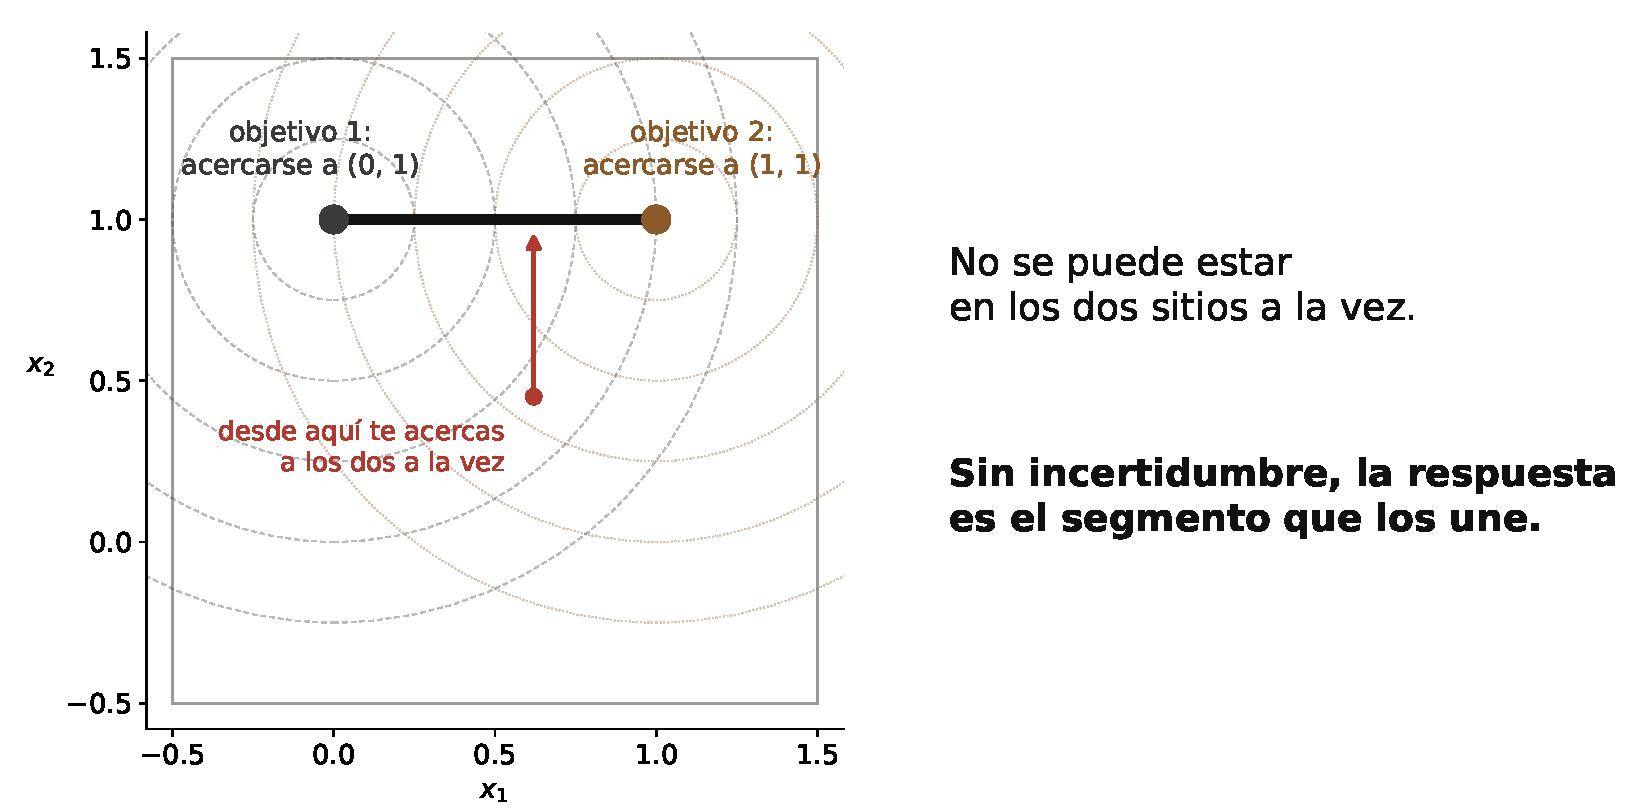
\includegraphics[width=0.99\textwidth,height=0.70\textheight,keepaspectratio]{p1_crisp.pdf}

  \vspace{-2mm}
  {\footnotesize Dos variables, un problema que se puede resolver a mano.}
  \NotaVI
\end{frame}

% ---------------------------------------------------------------- 7
\begin{frame}{p1, tres órdenes, tres respuestas distintas}
  \centering
  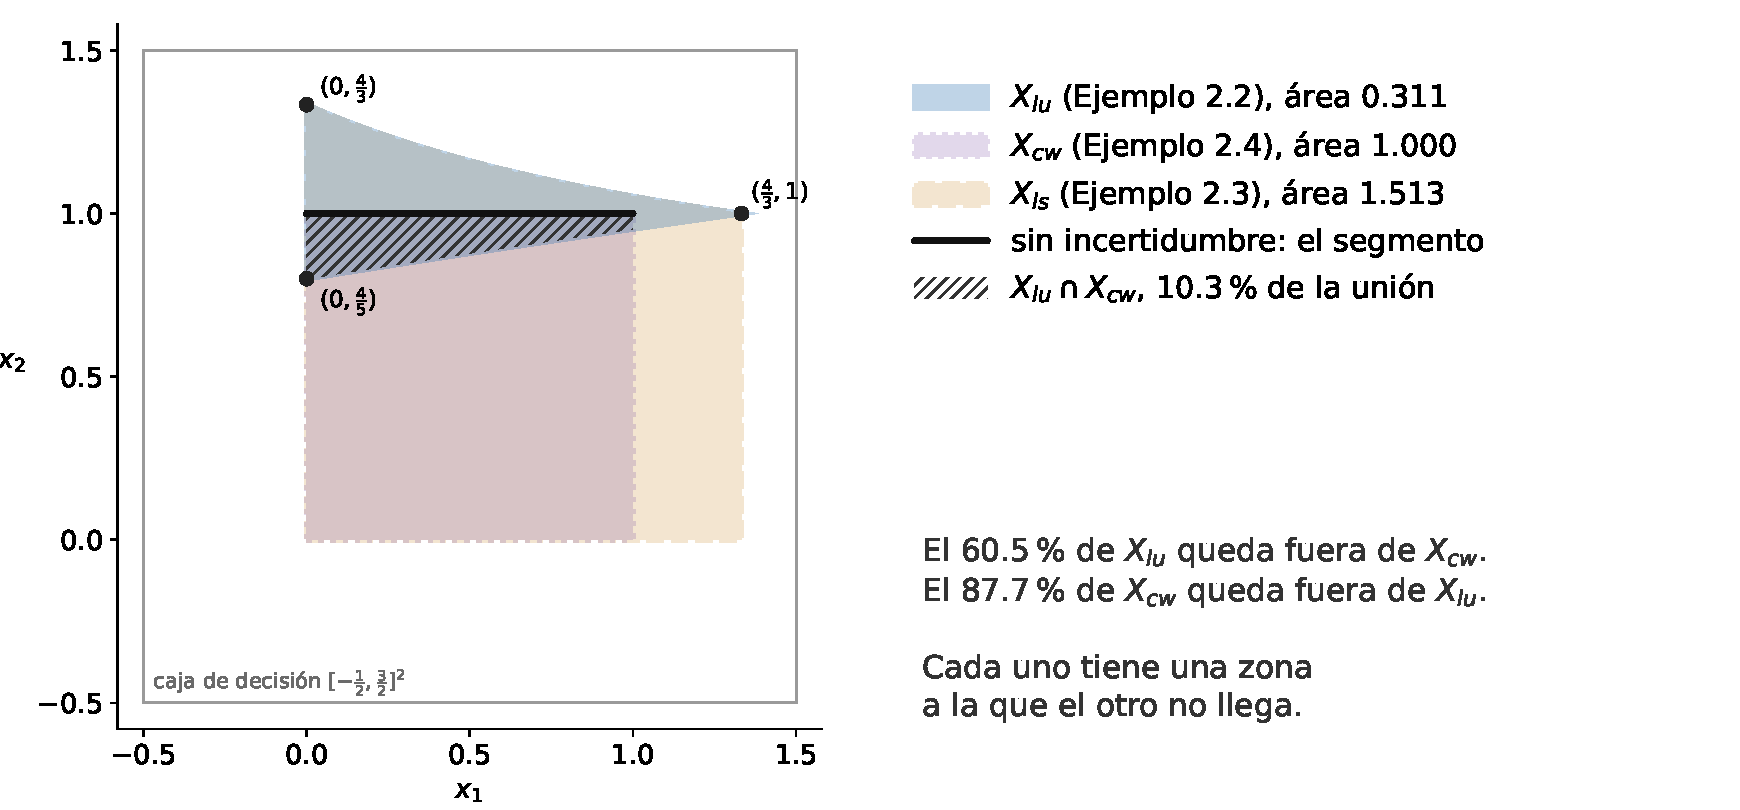
\includegraphics[width=0.98\textwidth,height=0.70\textheight,keepaspectratio]{p1_regiones.pdf}

  \vspace{-2mm}
  {\footnotesize De todo lo que podrían tener en común, sólo comparten el
  \textbf{\pUnionShare\,\%}. \cita{Y esto no lo ha calculado un ordenador: son las tres fórmulas dibujadas.}}
  \NotaVII
\end{frame}

% ---------------------------------------------------------------- 8
\begin{frame}{Y sé cuánto se equivoca lo que uso para medir}
  \centering
  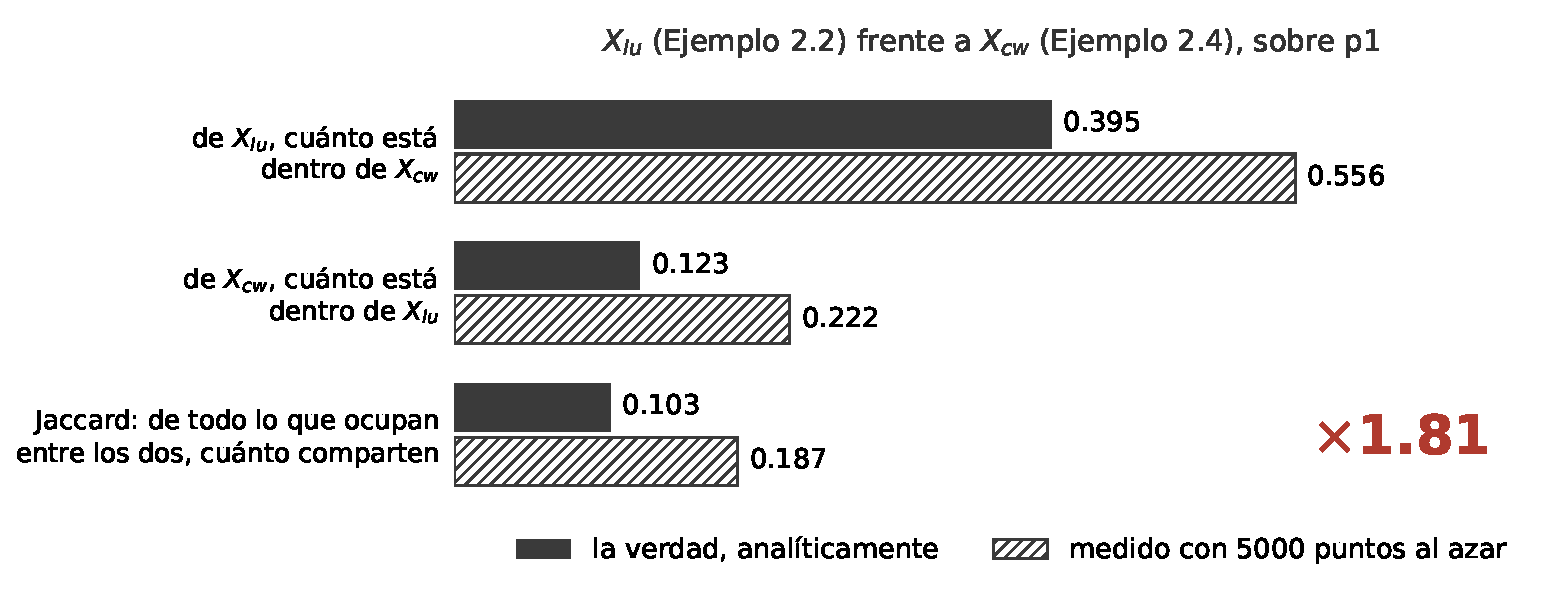
\includegraphics[width=0.97\textwidth,height=0.68\textheight,keepaspectratio]{instrumento.pdf}

  \vspace{-1mm}
  {\small Siempre en la misma dirección: al medir con puntos al azar, los dos
  órdenes salen \textbf{más parecidos de lo que son}.}
  \NotaVIII
\end{frame}

% ---------------------------------------------------------------- 9
\begin{frame}{Y ahora, p2, problemas de referencia del campo}
  \begin{columns}[T,onlytextwidth]
    \begin{column}{0.49\textwidth}
      \centering
      {\large\textbf{\ZdtName}} \quad \cita{\ZdtSize}\\[1mm]
      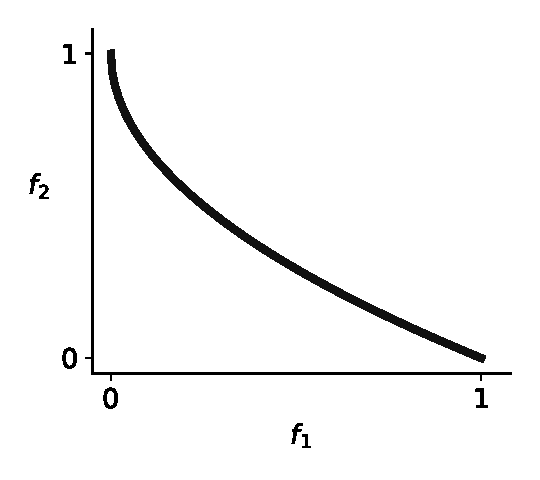
\includegraphics[height=0.33\textheight]{zdt1_frente.pdf}\\[-2mm]
      {\scriptsize $\ZdtF$\\[1mm] $\ZdtG$\\[0.5mm] \phantom{$\ZdtG$}}
    \end{column}
    \begin{column}{0.49\textwidth}
      \centering
      {\large\textbf{\DtlzName}} \quad \cita{\DtlzSize}\\[1mm]
      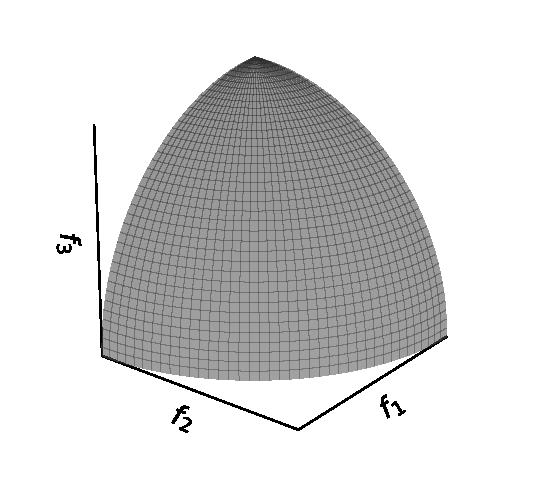
\includegraphics[height=0.33\textheight]{dtlz2_frente.pdf}\\[-2mm]
      {\scriptsize $\DtlzFone$\\[0.5mm] $\DtlzFtwo$\\[0.5mm] $\DtlzFthree$\\[1mm] $\DtlzG$}
    \end{column}
  \end{columns}
  \vspace{1mm}
  \begin{center}
    {\scriptsize Y a cada objetivo, su banda: \quad
    $\ZdtR$ \quad y \quad $\DtlzR$,\\[1mm]
    con $\marca{x_d}$ una variable que no está en el centro
    \cita{($\ZdtDrivers$ y $\DtlzDrivers$)} --- la regla de antes.}
  \end{center}
  \NotaIX
\end{frame}

% ---------------------------------------------------------------- 10
\begin{frame}{En p2: lo que te daba un orden, desaparece con el otro}
  \begin{columns}[c,onlytextwidth]
    \begin{column}{0.30\textwidth}
      \centering
      \begin{tikzpicture}[font=\tiny,scale=0.85,
          caja/.style={draw,rounded corners,minimum height=5mm,minimum width=18mm,align=center},
          filtro/.style={draw,rounded corners,minimum height=5mm,minimum width=13mm,align=center,thick},
          node distance=2.5mm and 4mm]
        \node[caja] (sample) {5000 puntos\\al azar};
        \node[caja,below=of sample] (eval) {una sola\\evaluación};
        \node[filtro,draw=phils,below=9mm of eval,xshift=4mm] (fls) {\pls};
        \node[filtro,draw=philu,below=of fls] (flu) {\plu};
        \node[filtro,draw=phicw,below=of flu] (fcw) {\pcw};
        \draw[-{Stealth}] (sample) -- (eval);
        % un carril a la izquierda, para que ninguna flecha cruce un cuadro
        \coordinate (lane) at ([xshift=-5mm]fls.west);
        \draw (eval.south) -- ++(0,-3mm) -| (lane);
        \draw (lane) -- (lane|-fcw.west);
        \draw[-{Stealth}] (lane|-fls.west) -- (fls.west);
        \draw[-{Stealth}] (lane|-flu.west) -- (flu.west);
        \draw[-{Stealth}] (lane|-fcw.west) -- (fcw.west);
        \node[below=3mm of fcw,align=center,gris,xshift=-2mm] {la misma lista, filtrada tres veces:\\lo único que cambia es el orden};
      \end{tikzpicture}
    \end{column}
    \begin{column}{0.68\textwidth}
      \centering
      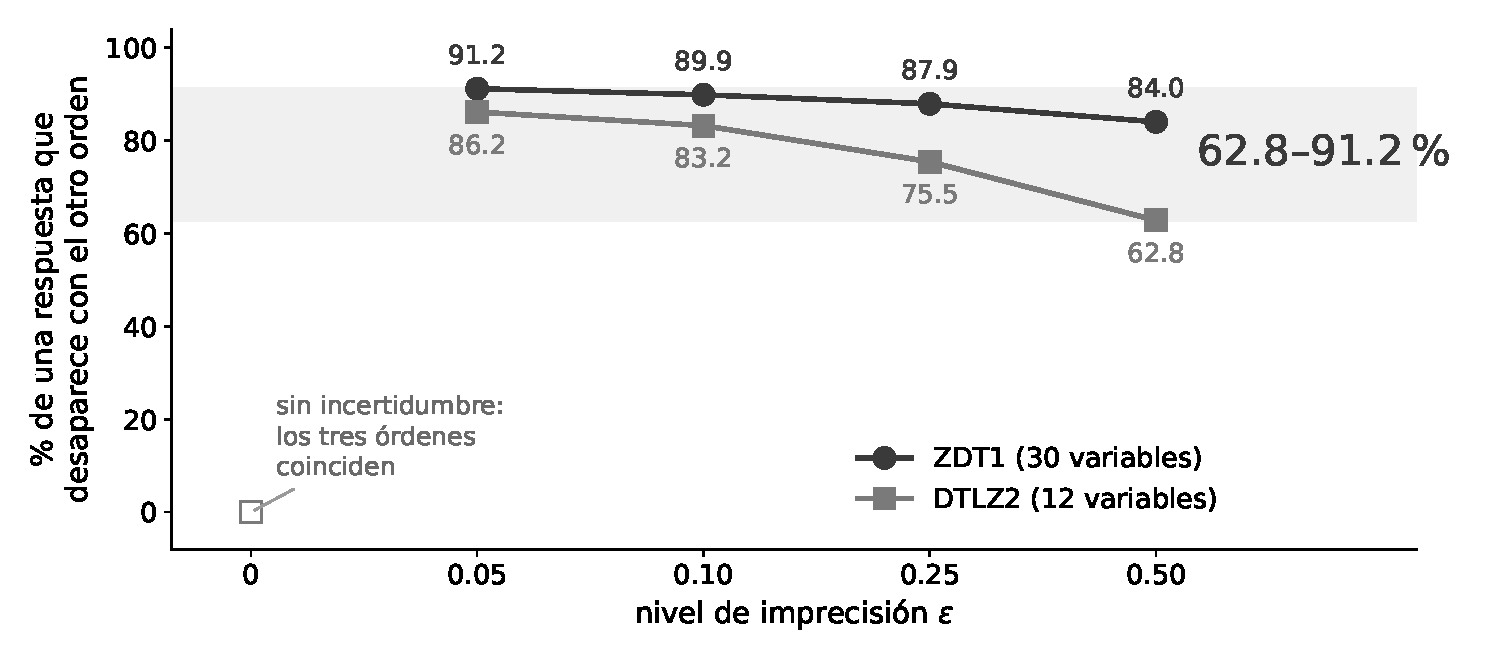
\includegraphics[width=0.98\textwidth,height=0.62\textheight,keepaspectratio]{benchmarks.pdf}
    \end{column}
  \end{columns}
  {\footnotesize Y como sé que mi medida dice que se parecen más de lo que se parecen, esto es un \textbf{mínimo}:
  \\ La diferencia real es mayor.}
  \NotaX
\end{frame}

% ---------------------------------------------------------------- 11
\begin{frame}{Y el tercero no lo he construido yo: está publicado}
  \centering
  \vspace{-2mm}
  {\footnotesize $\IBKone$,\quad $\IBKtwo$,\quad $x\in\IBKbox$}

  \vspace{-1mm}
  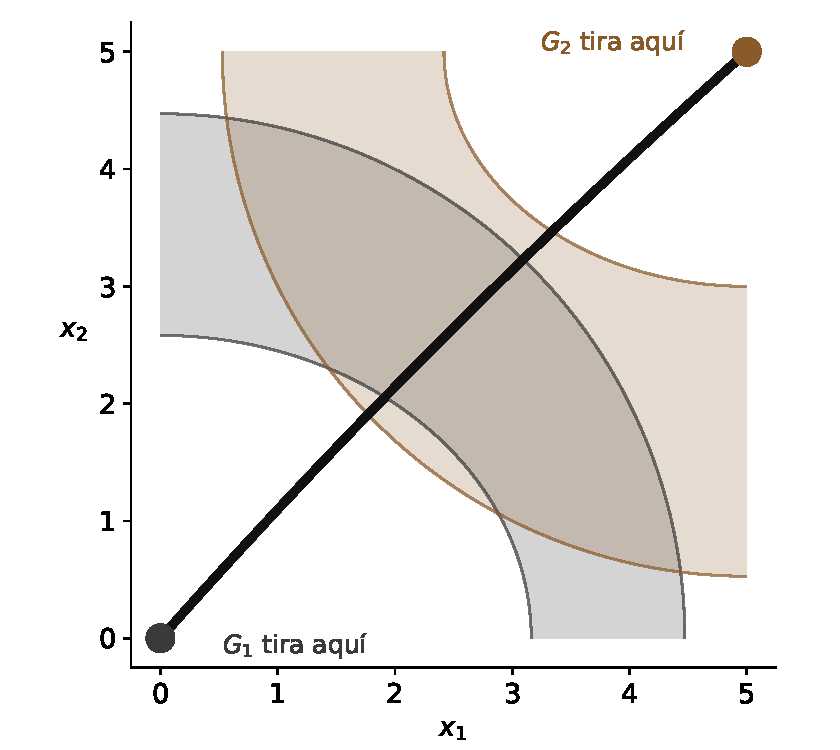
\includegraphics[height=0.69\textheight,keepaspectratio]{ibk1_crisp.pdf}

  \vspace{-1mm}
  {\footnotesize Cada objetivo vale un intervalo.}
  \NotaXI
\end{frame}

% ---------------------------------------------------------------- 12
\begin{frame}{Tres órdenes, tres respuestas: otra vez, y sin tocar el problema}
  \centering
  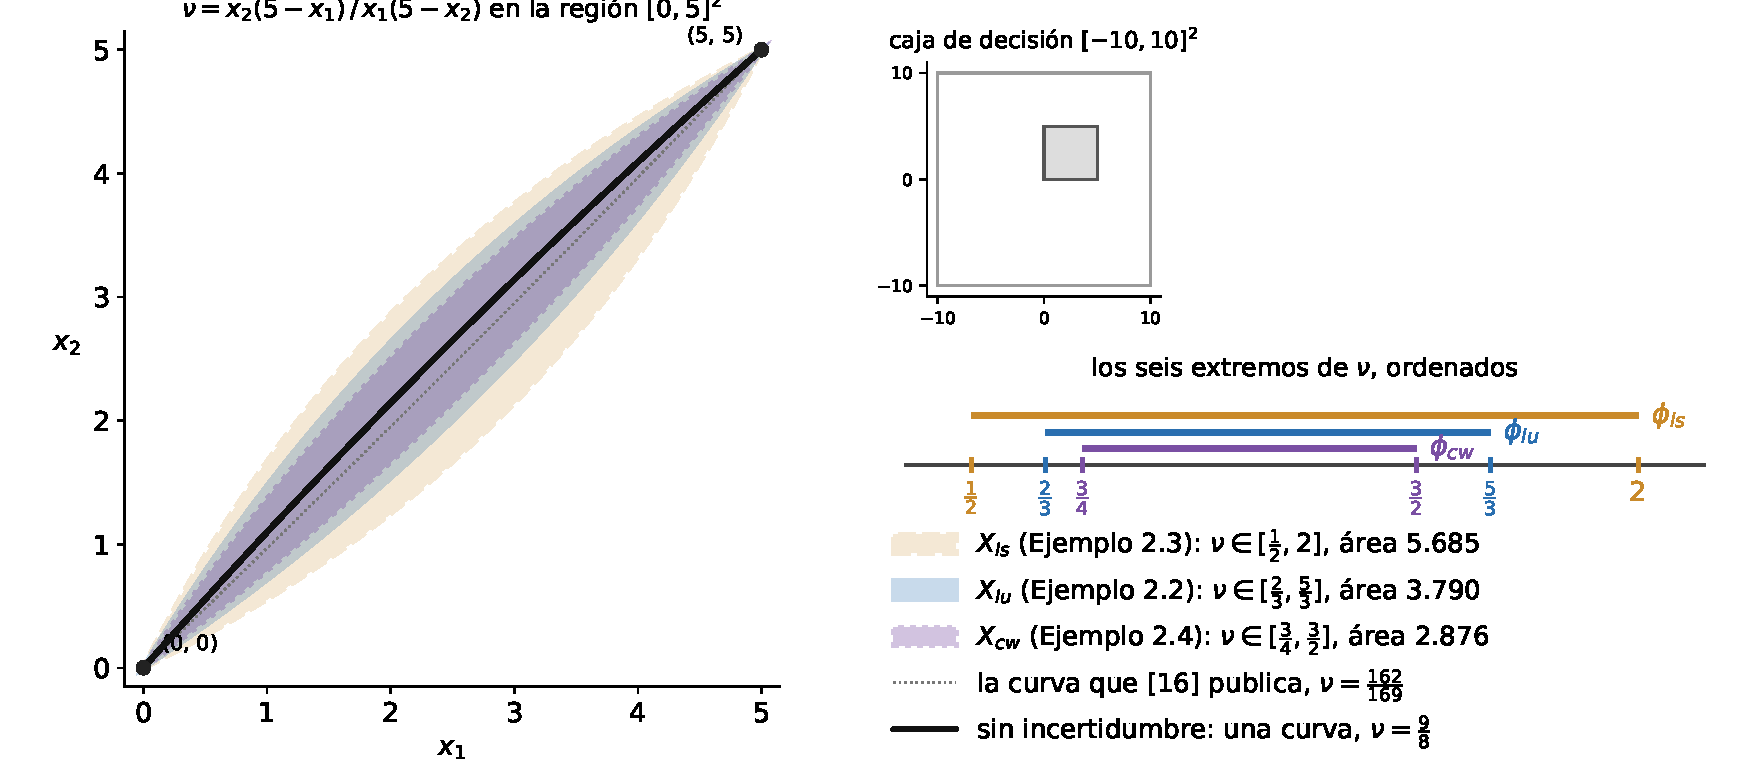
\includegraphics[width=0.98\textwidth,height=0.63\textheight,keepaspectratio]{ibk1_cunas.pdf}

  \vspace{-2mm}
  {\footnotesize Aquí las tres se meten una dentro de otra en vez de cruzarse: el
  \bMinInt--\bMaxInt\,\% de antes no vale aquí.\\ Lo que sí es
  exacto: el \textbf{\iLsOutsideCw\,\%} de la mayor queda fuera de la menor.}
  \NotaXII
\end{frame}

% ---------------------------------------------------------------- 13
\begin{frame}{Y de paso: el punto que publican como óptimo no lo es}
  \centering
  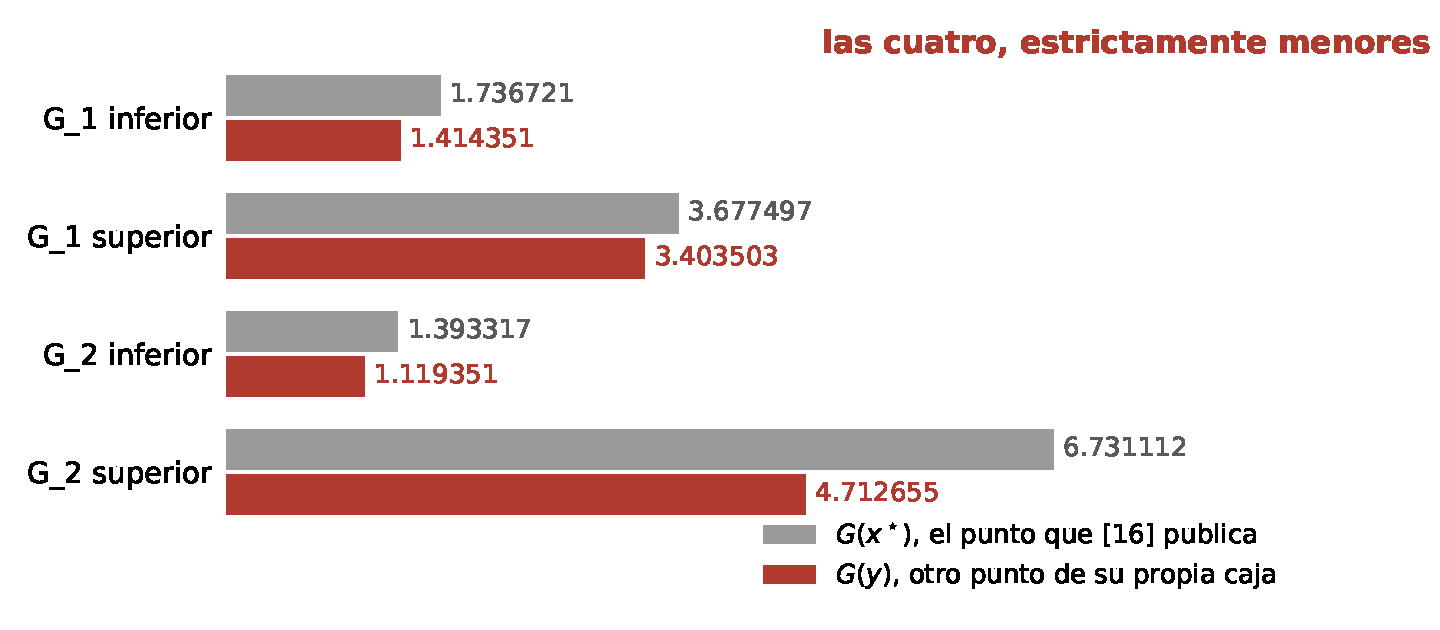
\includegraphics[width=0.88\textwidth,height=0.70\textheight,keepaspectratio]{contraejemplo.pdf}

  \vspace{-1mm}
  {\small Los de arriba son sus números; los de abajo salen con una calculadora
  en dos minutos.\\ \cita{Y los tres algoritmos lo encuentran.}}
  \NotaXIII
\end{frame}

% ---------------------------------------------------------------- cierre
\begin{frame}{Conclusiones}
  \vspace{4mm}
  \begin{center}
    \begin{minipage}{0.88\textwidth}
      {\large Elegir el orden no es un detalle de cómo montas el problema:\\
      \textbf{si no que condiciona la respuesta}.}
    \end{minipage}
  \end{center}
  \vspace{8mm}
  \begin{columns}[T,onlytextwidth]
    \begin{column}{0.32\textwidth}
      \centering
      {\LARGE\textbf{\pUnionShare\,\%}}\\[3mm]
      {\small es todo lo que dos órdenes\\ tienen en común}\\[2mm]
    \end{column}
    \begin{column}{0.32\textwidth}
      \centering
      {\LARGE\textbf{\bMinInt--\bMaxInt\,\%}}\\[3mm]
      {\small de tu respuesta desaparece\\ si te pasas al otro orden}\\[2mm]
    \end{column}
    \begin{column}{0.32\textwidth}
      \centering
      {\LARGE\textbf{\iLsOutsideCw\,\%}}\\[3mm]
      {\small de la respuesta mayor\\ se queda fuera de la menor}\\[2mm]
    \end{column}
  \end{columns}
  \vspace{7mm}
  \begin{center}
    \cita{Y siempre depende del problema: cada cifra viene de un problema concreto.}
  \end{center}
  \NotaXIV
\end{frame}

% ---------------------------------------------------------------- líneas futuras
\begin{frame}{Líneas futuras}
  \vspace{10mm}
  \begin{center}
    \begin{minipage}{0.82\textwidth}
      {\large
      \textbf{La curva de sensibilidad}: ir pasando poco a poco de un orden a
      otro, y ver cómo se mueve la respuesta.\\[8mm]
      \textbf{La aplicación a optimización de carteras}}
    \end{minipage}
  \end{center}
  \NotaXV
\end{frame}

\begin{frame}[plain]
  \vspace{10mm}
  \begin{center}
    {\Huge Gracias}\\[10mm]
  \end{center}
\end{frame}
\end{document}"
%                                                               -> presentacion_notas.pdf
\documentclass[aspectratio=169,11pt]{beamer}

\usetheme[numbering=fraction,progressbar=none,block=fill,background=light]{metropolis}
\usepackage[spanish,es-noshorthands,es-nodecimaldot]{babel}
\usepackage{amsmath,amssymb}
\usepackage{booktabs}
\usepackage{array}
\usepackage{tikz}
\usetikzlibrary{arrows.meta,positioning,calc,patterns,decorations.pathreplacing,shapes.geometric}
\usepackage{pgfpages}
\usepackage{appendixnumberbeamer}

% notas del orador: activadas con \def\shownotes{1} antes de \input
\ifdefined\shownotes
  \setbeameroption{show notes on second screen=right}
  \setbeamertemplate{note page}[plain]
  \setbeamerfont{note page}{size=\scriptsize}
\fi

% ---------------------------------------------------------------- colores
% Los tres órdenes llevan el mismo color en toda la presentación, y son los mismos
% tres valores hexadecimales que experiments/make_presentation.py usa en las
% figuras. Ninguno se lee como bueno o malo. La intersección se raya, nunca lleva
% un cuarto color.
\definecolor{philu}{HTML}{2A6FB0}
\definecolor{phils}{HTML}{C98A2B}
\definecolor{phicw}{HTML}{7A4FA3}
\definecolor{coefcol}{HTML}{B03A2E}
\definecolor{gris}{HTML}{6A6A6A}
\definecolor{grisclaro}{HTML}{DDDDDD}
\setbeamercolor{alerted text}{fg=coefcol}
\setbeamerfont{title}{size=\Large}

\newcommand{\plu}{\textcolor{philu}{$\phi_{lu}$}}
\newcommand{\pls}{\textcolor{phils}{$\phi_{ls}$}}
\newcommand{\pcw}{\textcolor{phicw}{$\phi_{cw}$}}
\newcommand{\Xlu}{\textcolor{philu}{$X_{lu}$}}
\newcommand{\Xls}{\textcolor{phils}{$X_{ls}$}}
\newcommand{\Xcw}{\textcolor{phicw}{$X_{cw}$}}
\newcommand{\coef}[1]{\textcolor{coefcol}{\boldsymbol{#1}}}
\newcommand{\marca}[1]{\textcolor{coefcol}{\boldsymbol{#1}}}
\newcommand{\cita}[1]{\textcolor{gris}{\small #1}}
\newcommand{\refuno}{[1] Costa, Osuna-Gómez y Chalco-Cano (2024)}
\newcommand{\refdieciseis}{[16] Mondal, Ghosh y Kim (2026)}

% ---------------------------------------------------------------- números generados
\graphicspath{{../results/figures/presentation/}}
% generated by experiments/make_presentation.py; do not edit.
% one \newcommand per number, each with the file and key it was read from.
% pRho: src/problems_tier0.py p1_default_params rho
\newcommand{\pRho}{\tfrac{1}{4}}
% pOffset: src/problems_tier0.py p1_default_params, the constant term of the half-width
\newcommand{\pOffset}{\tfrac{1}{8}}
% pBoxLo: src/problems_tier0.py p1_lower
\newcommand{\pBoxLo}{-\tfrac{1}{2}}
% pBoxHi: src/problems_tier0.py p1_upper
\newcommand{\pBoxHi}{\tfrac{3}{2}}
% pAreaLu: results/tier0/exact_regions_p1.csv area,lu
\newcommand{\pAreaLu}{0.311}
% pAreaLs: results/tier0/exact_regions_p1.csv area,ls
\newcommand{\pAreaLs}{1.513}
% pAreaCw: results/tier0/exact_regions_p1.csv area,cw
\newcommand{\pAreaCw}{1.000}
% pUnionShare: results/tier0/exact_regions_p1.csv overlap_union_share,lu,cw (in %)
\newcommand{\pUnionShare}{10.3}
% pLuOutsideCw: results/tier0/exact_regions_p1.csv 1 - coverage_a_in_b,lu,cw (in %)
\newcommand{\pLuOutsideCw}{60.5}
% pCwOutsideLu: results/tier0/exact_regions_p1.csv 1 - coverage_b_in_a,lu,cw (in %)
\newcommand{\pCwOutsideLu}{87.7}
% pCovLuCwExact: results/tier0/exact_regions_p1.csv coverage_a_in_b,lu,cw
\newcommand{\pCovLuCwExact}{0.395}
% pCovCwLuExact: results/tier0/exact_regions_p1.csv coverage_b_in_a,lu,cw
\newcommand{\pCovCwLuExact}{0.123}
% pJacExact: results/tier0/exact_regions_p1.csv overlap_union_share,lu,cw
\newcommand{\pJacExact}{0.103}
% pCovLuCwMeas: results/tier0/instrument_error_p1.csv (lu,cw; delta 0.0; n_evals 5000) measured_median, metric coverage_a_in_b
\newcommand{\pCovLuCwMeas}{0.556}
% pCovLuCwErr: results/tier0/instrument_error_p1.csv (lu,cw; delta 0.0; n_evals 5000) measured/exact, metric coverage_a_in_b
\newcommand{\pCovLuCwErr}{+40.8\,\%}
% pCovLuCwErrLarge: results/tier0/table_2_measured.csv decision block (lu,cw; delta 0.0; n_evals 20000) median/exact, metric coverage_a_in_b
\newcommand{\pCovLuCwErrLarge}{+27.7\,\%}
% pCovCwLuMeas: results/tier0/instrument_error_p1.csv (lu,cw; delta 0.0; n_evals 5000) measured_median, metric coverage_b_in_a
\newcommand{\pCovCwLuMeas}{0.222}
% pCovCwLuErr: results/tier0/instrument_error_p1.csv (lu,cw; delta 0.0; n_evals 5000) measured/exact, metric coverage_b_in_a
\newcommand{\pCovCwLuErr}{+81.0\,\%}
% pCovCwLuErrLarge: results/tier0/table_2_measured.csv decision block (lu,cw; delta 0.0; n_evals 20000) median/exact, metric coverage_b_in_a
\newcommand{\pCovCwLuErrLarge}{+48.6\,\%}
% pJacMeas: results/tier0/instrument_error_p1.csv (lu,cw; delta 0.0; n_evals 5000) measured_median, metric overlap via jaccard = dice/(2-dice)
\newcommand{\pJacMeas}{0.187}
% pJacErr: results/tier0/instrument_error_p1.csv (lu,cw; delta 0.0; n_evals 5000) measured/exact, metric overlap
\newcommand{\pJacErr}{$\times$1.81}
% pJacErrLarge: results/tier0/table_2_measured.csv decision block (lu,cw; delta 0.0; n_evals 20000) median/exact, metric overlap
\newcommand{\pJacErrLarge}{$\times$1.49}
% pJacFactorPlain: results/tier0/instrument_error_p1.csv (lu,cw; delta 0.0; n_evals 5000) jaccard measured/exact
\newcommand{\pJacFactorPlain}{1.81}
% pJacFactorLargePlain: results/tier0/table_2_measured.csv decision block (lu,cw; delta 0.0; n_evals 20000) jaccard measured/exact
\newcommand{\pJacFactorLargePlain}{1.49}
% bMinPct: results/tier1/table_2_measured_eps_{0.05,0.1,0.25,0.5}.csv decision block, lu,cw, finding, coverage_b_in_a, n_evals 5000, delta 0.0: min over the eight cells of 1 - median (in %)
\newcommand{\bMinPct}{62.8}
% bMaxPct: results/tier1/table_2_measured_eps_{0.05,0.1,0.25,0.5}.csv decision block, lu,cw, finding, coverage_b_in_a, n_evals 5000, delta 0.0: max over the eight cells of 1 - median (in %)
\newcommand{\bMaxPct}{91.2}
% bMinInt: results/tier1/table_2_measured_eps_{0.05,0.1,0.25,0.5}.csv decision block, lu,cw, finding, coverage_b_in_a, n_evals 5000, delta 0.0: min, rounded to the integer
\newcommand{\bMinInt}{63}
% bMaxInt: results/tier1/table_2_measured_eps_{0.05,0.1,0.25,0.5}.csv decision block, lu,cw, finding, coverage_b_in_a, n_evals 5000, delta 0.0: max, rounded to the integer
\newcommand{\bMaxInt}{91}
% bZdtVars: src/problems_tier1.py zdt1_n_vars
\newcommand{\bZdtVars}{30}
% bDtlzVars: src/problems_tier1.py dtlz2_n_vars
\newcommand{\bDtlzVars}{12}
% cZdtCardCw: results/tier1/table_2_measured_eps_{0.05,0.1,0.25,0.5}.csv decision block, lu,cw, finding, coverage_b_in_a, n_evals 5000, delta 0.0: cardinality_b, constant over the four eps
\newcommand{\cZdtCardCw}{257}
% cZdtCardLu: results/tier1/table_2_measured_eps_{0.05,0.1,0.25,0.5}.csv decision block, lu,cw, finding, coverage_b_in_a, n_evals 5000, delta 0.0: cardinality_a over eps 0.05, 0.1, 0.25, 0.5
\newcommand{\cZdtCardLu}{26\,\to\,36\,\to\,53\,\to\,68}
% cDtlzCardCw: results/tier1/table_2_measured_eps_{0.05,0.1,0.25,0.5}.csv decision block, lu,cw, finding, coverage_b_in_a, n_evals 5000, delta 0.0: cardinality_b, constant over the four eps
\newcommand{\cDtlzCardCw}{1813}
% cDtlzCardLu: results/tier1/table_2_measured_eps_{0.05,0.1,0.25,0.5}.csv decision block, lu,cw, finding, coverage_b_in_a, n_evals 5000, delta 0.0: cardinality_a over eps 0.05, 0.1, 0.25, 0.5
\newcommand{\cDtlzCardLu}{278\,\to\,351\,\to\,575\,\to\,980}
% ZdtName: src/problems_tier1.py zdt1_interval
\newcommand{\ZdtName}{ZDT1}
% ZdtSize: src/problems_tier1.py zdt1_n_vars, zdt1_n_obj
\newcommand{\ZdtSize}{30 variables, 2 objetivos}
% ZdtF: src/problems_tier1.py evaluate_zdt1, [2] equations (6) and (7)
\newcommand{\ZdtF}{f_1 = x_1, \qquad f_2 = g\,\Bigl(1 - \sqrt{f_1/g}\,\Bigr)}
% ZdtG: src/problems_tier1.py evaluate_zdt1, g with m - 1 = zdt1_n_vars - 1
\newcommand{\ZdtG}{g = 1 + \dfrac{9}{29}\sum_{i \geq 2} x_i}
% ZdtR: src/problems_tier1.py zdt1_half_width
\newcommand{\ZdtR}{r_i = \varepsilon\,\bigl( (\marca{x_d} - \tfrac{1}{2})^2 + \tfrac{1}{20} \bigr)}
% ZdtDrivers: src/problems_tier1.py zdt1_width_drivers, as 1-based names
\newcommand{\ZdtDrivers}{x_{30}, x_{29}}
% DtlzName: src/problems_tier1.py dtlz2_interval
\newcommand{\DtlzName}{DTLZ2}
% DtlzSize: src/problems_tier1.py dtlz2_n_vars, dtlz2_n_obj
\newcommand{\DtlzSize}{12 variables, 3 objetivos}
% DtlzFone: src/problems_tier1.py evaluate_dtlz2, [3] equation (9) at M = 3
\newcommand{\DtlzFone}{f_1 = (1+g)\cos\tfrac{\pi x_1}{2}\cos\tfrac{\pi x_2}{2}}
% DtlzFtwo: src/problems_tier1.py evaluate_dtlz2, [3] equation (9) at M = 3
\newcommand{\DtlzFtwo}{f_2 = (1+g)\cos\tfrac{\pi x_1}{2}\sin\tfrac{\pi x_2}{2}}
% DtlzFthree: src/problems_tier1.py evaluate_dtlz2, [3] equation (9) at M = 3
\newcommand{\DtlzFthree}{f_3 = (1+g)\sin\tfrac{\pi x_1}{2}}
% DtlzG: src/problems_tier1.py evaluate_dtlz2, g over the tail
\newcommand{\DtlzG}{g = \sum_{i \geq 3} (x_i - \tfrac{1}{2})^2}
% DtlzR: src/problems_tier1.py dtlz2_half_width
\newcommand{\DtlzR}{r_i = \varepsilon\,\marca{x_d}}
% DtlzDrivers: src/problems_tier1.py dtlz2_width_drivers, as 1-based names
\newcommand{\DtlzDrivers}{x_{12}, x_{11}, x_{10}}
% IBKone: src/problems_native.py ibk1_coefficients[0]
\newcommand{\IBKone}{G_1 = \coef{[0.1, 0.2]}\, x_1^2 + \coef{[0.1, 0.3]}\, x_2^2}
% IBKtwo: src/problems_native.py ibk1_coefficients[1], ibk1_shift
\newcommand{\IBKtwo}{G_2 = \coef{[0.1, 0.3]}\, (x_1 - 5)^2 + \coef{[0.1, 0.5]}\, (x_2 - 5)^2}
% IBKbox: src/problems_native.py ibk1_lower, ibk1_upper
\newcommand{\IBKbox}{[-10, 10]^2}
% IBKratiosOne: computed from ibk1_coefficients[0]: (b-a)/(a+b) per term
\newcommand{\IBKratiosOne}{\tfrac{1}{3} frente a \tfrac{1}{2}}
% IBKratiosTwo: computed from ibk1_coefficients[1]: (b-a)/(a+b) per term
\newcommand{\IBKratiosTwo}{\tfrac{1}{2} frente a \tfrac{2}{3}}
% iAreaLu: results/part2/exact_regions_ibk1.csv area,lu
\newcommand{\iAreaLu}{3.790}
% iBandLuLo: results/part2/exact_regions_ibk1.csv band_lower,lu
\newcommand{\iBandLuLo}{\tfrac{2}{3}}
% iBandLuHi: results/part2/exact_regions_ibk1.csv band_upper,lu
\newcommand{\iBandLuHi}{\tfrac{5}{3}}
% iAreaLs: results/part2/exact_regions_ibk1.csv area,ls
\newcommand{\iAreaLs}{5.685}
% iBandLsLo: results/part2/exact_regions_ibk1.csv band_lower,ls
\newcommand{\iBandLsLo}{\tfrac{1}{2}}
% iBandLsHi: results/part2/exact_regions_ibk1.csv band_upper,ls
\newcommand{\iBandLsHi}{2}
% iAreaCw: results/part2/exact_regions_ibk1.csv area,cw
\newcommand{\iAreaCw}{2.876}
% iBandCwLo: results/part2/exact_regions_ibk1.csv band_lower,cw
\newcommand{\iBandCwLo}{\tfrac{3}{4}}
% iBandCwHi: results/part2/exact_regions_ibk1.csv band_upper,cw
\newcommand{\iBandCwHi}{\tfrac{3}{2}}
% iOrderedEnds: results/part2/exact_regions_ibk1.csv the six band ends, sorted
\newcommand{\iOrderedEnds}{\tfrac{1}{2} < \tfrac{2}{3} < \tfrac{3}{4} < \tfrac{3}{2} < \tfrac{5}{3} < 2}
% iLsOutsideCw: results/part2/exact_regions_ibk1.csv 1 - coverage_a_in_b,ls,cw (in %)
\newcommand{\iLsOutsideCw}{49.4}
% iCovLsCw: results/part2/exact_regions_ibk1.csv coverage_a_in_b,ls,cw
\newcommand{\iCovLsCw}{0.506}
% iNuCurve: docs/part2/f2_ibk1_derivation.md section 4.1, nu of equation (25)'s curve
\newcommand{\iNuCurve}{\tfrac{162}{169}}
% iCritRatio: docs/part2/f2_ibk1_derivation.md section 4.3, critical set measure over X_lu's
\newcommand{\iCritRatio}{4.24}
% iNuCrisp: computed from src/problems_native.py's coefficients and checked against docs/part2/f2_ibk1_derivation.md section 3.3
\newcommand{\iNuCrisp}{\tfrac{9}{8}}
% IVUone: [16] appendix A problem 2, as docs/part2/f7_ivu2_derivation.md transcribes it
\newcommand{\IVUone}{G_1 = \coef{[1, 1.5]}\, \marca{x_1} + \coef{[1, 1.5]}\, \marca{x_2} + \coef{[1, 1]}}
% IVUtwo: [16] appendix A problem 2, as docs/part2/f7_ivu2_derivation.md transcribes it
\newcommand{\IVUtwo}{G_2 = \coef{[1, 1.5]}\, x_1^2 + \coef{[2, 3]}\, x_2^2 - \coef{[1, 1]}}
% IVUbox: [16] appendix A problem 2, as docs/part2/f7_ivu2_derivation.md transcribes it
\newcommand{\IVUbox}{[-4, 4]^2}
% dXstar: [16] Table 1 page 20, as docs/part2/f2_ibk1_derivation.md section 4.2 (re-computed here in exact rationals from src/problems_native.py's coefficients and asserted equal)
\newcommand{\dXstar}{(3.914930, 1.428474)}
% dY: docs/part2/f2_ibk1_derivation.md section 4.2 (re-computed here in exact rationals from src/problems_native.py's coefficients and asserted equal)
\newcommand{\dY}{(2.8975, 2.3975)}
% dMinMargin: docs/part2/f2_ibk1_derivation.md section 4.2 (re-computed here in exact rationals from src/problems_native.py's coefficients and asserted equal): the smallest of the four margins
\newcommand{\dMinMargin}{0.274}
% dConfigs: results/part2/dominators_summary.csv: number of rows (solver x phi x budget)
\newcommand{\dConfigs}{18}
% dConfigsWithDominator: results/part2/dominators_summary.csv: rows with seeds_with_a_dominator == n_seeds
\newcommand{\dConfigsWithDominator}{18}
% dWidestMargin: results/part2/dominators_summary.csv: max of widest_margin_over_seeds
\newcommand{\dWidestMargin}{0.270}
% iJacFactorMin: results/part2/instrument_error_ibk1.csv, metric overlap, delta 0.0, jaccard = dice/(2-dice), measured/exact over the three pairs (min)
\newcommand{\iJacFactorMin}{1.01}
% iJacFactorMax: results/part2/instrument_error_ibk1.csv, metric overlap, delta 0.0, jaccard = dice/(2-dice), measured/exact over the three pairs (max)
\newcommand{\iJacFactorMax}{1.48}
% aCorrProportional: docs/part1/a1_uncertainty_model.md part 1, the proportional width, corr(centre, width)
\newcommand{\aCorrProportional}{+1.0000}
% rWidthValuesTrue: docs/explicacion_proyecto.md section 10.3
\newcommand{\rWidthValuesTrue}{46}
% rWidthValuesSeen: docs/explicacion_proyecto.md section 10.3
\newcommand{\rWidthValuesSeen}{210}
% rGridPoints: docs/explicacion_proyecto.md section 10.5
\newcommand{\rGridPoints}{40401}
% rFixedCoverage: instrument_error_p1.csv, instrument_error_ibk1.csv, table_2_measured_eps_*.csv: every check row with a containment-fixed direction
\newcommand{\rFixedCoverage}{1.000000}
% rFixedRange: same rows: q3 - q1
\newcommand{\rFixedRange}{0}
% rFixedRows: same rows: how many were checked
\newcommand{\rFixedRows}{28}
% rSatConfigs: results/tier1/rank_one_summary.csv: nsga2 rows with eps > 0 at n_evals 5000
\newcommand{\rSatConfigs}{24}
% rGenerations: results/tier1/rank_one_summary.csv: n_generations
\newcommand{\rGenerations}{50}

% generated by experiments/make_presentation.py from presentation/guion.txt
% one command per slide, in order; presentacion.tex uses them inside \note{}.
\newcommand{\NotaI}{\note{Optimizar es buscar el mejor valor de algo. Con un objetivo hay una respuesta: un punto. En la práctica casi nunca hay uno solo: quieres bajar el coste y bajar el riesgo, y se contradicen. Como optimizar un programa para que sea rápido y gaste poca memoria: no existe el mejor programa. Cuando hay varios objetivos ya no hay un ganador único: hay un conjunto de soluciones que no se pueden mejorar en un objetivo sin empeorar otro. Se llama conjunto eficiente, o frente de Pareto. La regla que lo define es la dominancia, la de la caja. Esto es todo lo que hace falta saber de optimización multiobjetivo}}
\newcommand{\NotaII}{\note{En la realidad no sabemos los valores exactos de las variables. El coste no es 40, es entre 38 y 45: hay un error de medida, hay parámetros que varían, información incompleta. Un intervalo es eso. Tres palabras que hay que fijar ya: centro, semianchura y anchura. Y los objetivos ahora son intervalos, dejan de poder ordenarse. Con A=(1’5 , 5) y =(3,7’5) A parece menor. Pero con A igual a uno a diez y B igual a cuatro a cinco, A puede ser mejor o mucho peor. No hay respuesta. No es un problema técnico: es que no existe una única forma correcta de ordenar intervalos. Existen muchas, y cada una es una decisión sobre qué te importa.}}
\newcommand{\NotaIII}{\note{El primer artículo de Rafaela … , hizo algo elegante: en vez de proponer un orden, describió toda la familia de órdenes posibles, con un parámetro que dice cuál estás usando. Ese parámetro es fi. Un fi coge un intervalo y devuelve dos números reales, que sí se pueden comparar. Los tres que el artículo nombra: fi\_Lu, compara mejor caso con mejor caso y peor con peor fi\_Ls, extremo inferior y anchura; fi\_cw, centro y semianchura. Los tres son válidos, distintos, y cada uno da un conjunto eficiente distinto. Analogía: fi es la función clave de un sort. La regla: m objetivos intervalares se convierten en dos m objetivos reales, y eso ya se sabe resolver con NSGA-II o PSO. El artículo demuestra que resolver el transformado equivale a resolver el original}}
\newcommand{\NotaIV}{\note{Y con esto ya puedo decir qué es lo que me pregunto, que es una sola cosa: si cambio el orden y no cambio nada más, ¿cambia la respuesta? ¿Y cuánto? Hay otra pregunta que la gente hace enseguida y que yo no contesto: cuál de los tres órdenes es el bueno. No la contesto porque no se puede con lo que tengo delante. Cada orden mira el problema a su manera, y para decir cuál acierta haría falta saber qué pasa de verdad después, en la realidad. Estos problemas de prueba no lo dicen. Prefiero decirlo yo ahora y no que se quede la duda.}}
\newcommand{\NotaV}{\note{Lo primero que hice fue lo obvio, y salió mal. Es el hallazgo del que más he aprendido. Cogí un problema normal y le puse un margen de error fijo arriba y abajo: en vez de un número, un intervalo de ancho siempre igual. Parece sensato y es inútil. Si todos los intervalos tienen el mismo ancho, dos de los tres órdenes están mirando un número que nunca cambia. Y un dato que es siempre el mismo no sirve para ordenar nada: es como ordenar una lista de gente por el número siete. Resultado: los tres órdenes daban exactamente el mismo conjunto, y encima el mismo que si no hubiera incertidumbre. Y no lo deduje, lo medí: los tres conjuntos salieron con los mismos puntos, uno por uno. De aquí sale la regla que gobierna todo lo demás: la incertidumbre tiene que depender de algo que el valor central no controle. Si el ancho se puede calcular a partir del centro, los tres órdenes se vuelven el mismo. Si hubiera montado el estudio sin darme cuenta de esto, todas mis tablas habrían salido llenas de unos y habría concluido que el orden da igual. Que es justo lo contrario de la verdad.}}
\newcommand{\NotaVI}{\note{Antes de enseñaros lo que sale, un minuto con el problema, porque si no la siguiente imagen no se entiende. Me construí un problema de dos variables, a medida, para poder resolverlo a mano. Los dos objetivos son lo mismo: acércate a un punto. Uno te pide acercarte a éste y el otro a éste de aquí. Si sólo tuviera el primero, la respuesta sería ese punto, y ya está. Si sólo tuviera el segundo, el otro. Pero no puedo estar en los dos sitios a la vez. Y fijaos en lo que pasa con cualquier punto que no esté en la línea: si tiro hacia la línea me acerco a los dos objetivos a la vez, así que ese punto no puede ser una respuesta, porque hay otro mejor en todo. Conclusión: sin incertidumbre, la respuesta de este problema es exactamente el segmento que une los dos puntos. Una línea. Quedaos con esa línea, porque ahora le voy a meter la incertidumbre y vamos a ver qué le pasa.}}
\newcommand{\NotaVII}{\note{Así que me construí un problema a medida, con dos variables, para poder resolverlo a mano. Tiene dos objetivos, y la gracia está en el cruce: la incertidumbre de cada objetivo depende de la variable del otro. Que es la regla de antes, aplicada. Y como todo es cuadrático, las condiciones de optimalidad se convierten en un sistema de ecuaciones que se resuelve con papel y lápiz. Usando el Teorema 3.3 y el Ejemplo 3.9 del artículo de Rafaela — sus propios resultados, aplicados, no inventados por mí — saco la respuesta exacta bajo cada uno de los tres órdenes. Y esto es lo que sale. Esto no es lo que me ha devuelto un ordenador: son las tres fórmulas dibujadas. No hay muestreo ni algoritmo dentro. Los dos ejes son las dos variables. El cuadrado es la respuesta con un orden, la región grande con otro, la lente con el tercero. Mismo problema, mismos datos; lo único que cambia es el orden. Y mirad lo que pasa: la lente y el cuadrado no se contienen. La lente sube por arriba, donde el cuadrado no llega; el cuadrado ocupa todo lo de abajo, donde la lente no llega. Cada uno tiene una zona a la que el otro no alcanza. De todo lo que podrían tener en común, sólo comparten el diez por ciento. Y esto es exacto, medido sobre las fórmulas. Si alguien está eligiendo entre soluciones, cambiar de orden le cambia casi toda la lista.}}
\newcommand{\NotaVIII}{\note{Ahora, en un problema así yo tengo la respuesta exacta. Pero en un problema de verdad no la voy a tener: voy a tener lo que me devuelva el ordenador. Así que aproveché: tengo las dos cosas a la vez, lo exacto y lo medido, y las puse una al lado de la otra. Esto es algo que casi ningún trabajo tiene: sé cuánto se equivoca mi propio instrumento. Y se equivoca siempre en la misma dirección: dice que los dos órdenes se parecen más de lo que se parecen. Donde de verdad comparten un diez por ciento, él dice dieciocho. La razón es fácil de ver: cuando pruebas puntos al azar, encuentras primero los fáciles, y los fáciles son justo los que están en la zona común. Lo que pertenece a un solo conjunto está en los bordes y cuesta más pillarlo. Ese factor, casi el doble, es de este problema. No lo llevo a ningún otro sitio ni corrijo ningún número con él.}}
\newcommand{\NotaIX}{\note{Hasta aquí todo ha sido un problema de dos variables que me inventé yo. Toca salir a problemas de verdad. Éstos son dos de los que se usan como referencia en el campo: ZDT1 y DTLZ2. No son míos: están publicados y todo el mundo los conoce. El primero tiene treinta variables y dos objetivos, y su respuesta, sin incertidumbre, es esa curva. El segundo tiene doce variables y tres objetivos, y su respuesta es ese trozo de esfera. Fijaos en el salto: antes la respuesta era un segmento en un plano que cabía en una imagen; aquí ya no puedo dibujar el espacio de las soluciones, porque tiene treinta dimensiones. A los dos les pongo una banda de incertidumbre encima, con la regla del principio: la anchura la mueve una variable que no está en el centro. Está marcada en rojo. Y el parámetro épsilon es cuánta imprecisión les meto. Voy a probar cuatro niveles.}}
\newcommand{\NotaX}{\note{Aquí está el método, y es lo que hace que el número de la derecha valga algo. Va de arriba abajo, por el esquema de la izquierda. Uno: cojo cinco mil puntos al azar dentro de la caja. Al azar de verdad, sin mirar los objetivos y sin usar nada de lo que sé del problema. Dos: evalúo esos cinco mil puntos una sola vez. Cada punto me devuelve sus intervalos, uno por objetivo, y esa lista ya no se vuelve a tocar. Tres: cojo esa única lista y la filtro tres veces. En cada pasada uso uno de los tres órdenes: comparo los puntos entre sí con ese criterio y me quedo con los que no domina nadie. Tres pasadas sobre la misma lista, tres subconjuntos. Y aquí está la gracia: los tres salen de los mismos puntos y de los mismos números; lo único distinto es el criterio con el que comparo. Así que cualquier diferencia entre ellos es del orden y de nada más. Si lanzara un algoritmo evolutivo tres veces, una con cada orden, cambiaría dos cosas a la vez: el criterio, que es lo que quiero medir, y por dónde busca el algoritmo. Saldrían mezcladas y no podría separarlas. Por eso probar al azar no es el rival flojo: es el instrumento con el que mido. NSGA-II y el PSO multiobjetivo sí están en el trabajo, pero en otro sitio: comprobando que los solvers llegan a donde la derivación dice, y en la última diapositiva. Y esto es lo que sale: entre el sesenta y tres y el noventa y uno por ciento de lo que te daba un orden desaparece si te pasas al otro. Y como ya sé que mi instrumento exagera el parecido, esto es un mínimo: la diferencia real es mayor. No están inflados a mi favor, sino en mi contra. Abajo a la izquierda, la comprobación: sin incertidumbre, los tres órdenes vuelven a dar lo mismo.}}
\newcommand{\NotaXI}{\note{Llegados aquí alguien puede decirme, con toda la razón: claro, te has construido tú el problema para que salga lo que querías. Y es verdad, y por eso está medido y escrito. Así que el tercer problema no lo he tocado yo. Está publicado por otros autores, para otra cosa, antes de que yo empezara. Y es intervalar de origen: los intervalos están en los propios coeficientes, ahí arriba, entre corchetes. Yo no elegí ni cuánto valen ni de qué variable dependen. Por dentro es el mismo tipo de problema que el mío: dos objetivos, y cada uno te pide acercarte a una esquina. Uno tira hacia el cero y el otro hacia el cinco cinco. Con una diferencia que se ve en el dibujo: como los coeficientes son intervalos, un objetivo ya no vale un número. Pedirle que valga dos no te da una curva, te da esa banda sombreada. Y como antes: si quito la incertidumbre y me quedo con los valores centrales, la respuesta es una sola curva, la negra. Quedaos otra vez con esa curva.}}
\newcommand{\NotaXII}{\note{Y esto es lo que sale al derivarlo a mano, que es más bonito de lo que esperaba: toda la respuesta cabe en un solo número. Cada orden se queda con los puntos cuyo número cae dentro de un intervalo, y el intervalo depende del orden. Tres cuñas, ancladas en las mismas dos esquinas, con la curva de antes por el medio. Otra vez tres órdenes, tres respuestas distintas, en un problema que no es mío. Y fijaos en el salto: sin incertidumbre era una curva; con cada orden es una región con superficie. Pero aquí tengo que ser honesto con una cosa: estas tres se meten una dentro de otra, no se cruzan como antes. Así que el número del sesenta y tres al noventa y uno no tiene equivalente aquí, y no lo reclamo. Lo que sí puedo decir es que la mitad de la mayor se queda fuera de la menor. Y hay una comprobación que no es mía y que sale bien: ellos publican una curva de soluciones, la calculo, y cae dentro de las tres cuñas. Un apunte más, porque marca el límite: derivé un segundo problema suyo y ahí los tres órdenes dan exactamente lo mismo. O sea que ser un problema intervalar de verdad no basta para que el orden importe. Se sabe mirando los coeficientes, antes de resolver nada.}}
\newcommand{\NotaXIII}{\note{Y esto salió de paso. No me puse a buscar errores en nadie: me puse a comprobar mi propia derivación contra lo que ellos publican, que es lo que hay que hacer. Ellos dan este punto como solución óptima de su problema. Su propia definición dice qué significa eso: que no exista otro punto que sea igual o mejor en las cuatro cantidades. Cogí otro punto, que está dentro de su misma caja, y lo comparé con los números que ellos imprimen. Las cuatro salen menores. Las cuatro. Los de arriba son sus números, tal como están en el artículo; los de abajo se calculan con una calculadora en dos minutos. No hace falta creerse nada de lo que yo he hecho. Y no es cosa del redondeo: la diferencia más ajustada es doscientas mil veces mayor que lo que podría moverse el último decimal que ellos imprimen. Además, los tres algoritmos lo encuentran solos. A la sesión que los lanzó no se le dijo nada de este punto, y las dieciocho configuraciones devolvieron puntos que lo ganan. Es una corrección, no una crítica. Y lo que no digo es dónde está el fallo de su demostración: se apoya en otro artículo suyo que yo no tengo. Digo que la conclusión es falsa; no digo por qué.}}
\newcommand{\NotaXIV}{\note{Y resumo con lo que defiendo, que es una sola cosa: elegir el orden no es un detalle de cómo montas el problema, es media respuesta. Con tres medidas. En mi problema, hecho a mano y exacto: de todo lo que podrían tener en común dos órdenes, sólo comparten el diez por ciento. En dos problemas de referencia del campo, medido: entre el sesenta y tres y el noventa y uno por ciento de lo que te daba un orden desaparece si te pasas al otro. Y con un instrumento cuyo error conozco, así que eso es un mínimo. Y en un problema publicado por otros, que no he tocado yo: la mitad de la respuesta mayor se queda fuera de la menor. Todo esto bajo una condición sobre el modelo de incertidumbre que no supuse, sino que medí, y que además se puede comprobar en cualquier problema antes de ponerse a resolver. Y tres cosas que no sé, y que están escritas: por qué a uno de los algoritmos le cuesta más de lo que debería, después de descartar cinco explicaciones midiéndolas; por qué en un problema las respuestas se cruzan y en otro se anidan; y por qué mi instrumento se equivoca casi el doble en un problema y casi nada en otro. Que esas tres estén escritas es parte del resultado, no un defecto.}}
\newcommand{\NotaXV}{\note{Y lo que queda por hacer, que son dos cosas. La primera es la curva de sensibilidad: en vez de tres órdenes sueltos, ir pasando poco a poco de uno a otro y ver cómo se mueve la respuesta. Es admisible por la propia definición del artículo y el código está montado para que sea un bucle; fue lo primero que me quité de encima por falta de tiempo, y es la mejora más grande que hay disponible. Y la segunda son las carteras, que es donde vuestra propia propuesta las pone, como trabajo futuro. Gracias.}}


\title{Técnicas de Optimización Intervalar basadas en Inteligencia Computacional}
\subtitle{¿Cuánto cambia la respuesta cuando lo único que cambia es el orden?}
\author{Francisco Rodríguez-Carretero Roldán}
\institute{Tutores: Antonio Beato Moreno y Rafaela Osuna Gómez · Universidad de Sevilla}
\date{25 de septiembre de 2026 · Proyecto PI3, julio--septiembre 2026}

\begin{document}

% ================================================================ portada
\begin{frame}[plain]
  \vspace{-6mm}\titlepage
\end{frame}

% ================================================================ BLOQUE A
% ---------------------------------------------------------------- 1
\begin{frame}{Optimizar con varios objetivos: no hay un ganador, hay un conjunto}
  \begin{columns}[T]
    \begin{column}{0.52\textwidth}
      \centering
      \begin{tikzpicture}[scale=0.55]
        \draw[-{Stealth}] (0,0) -- (10.5,0) node[below left] {coste};
        \draw[-{Stealth}] (0,0) -- (0,9.5) node[below right,rotate=0] {riesgo};
        % dominados
        \foreach \x/\y in {3/7, 5/6, 6/4.5, 8/4, 4/6.5, 7/3.5, 9/5, 2.5/8.5, 5.5/8, 8.5/6.5, 3.5/5.5, 6.5/6}
          \fill[gris!60] (\x,\y) circle (0.14);
        % no dominados
        \draw[dashed,gris] plot[smooth] coordinates {(1,8) (2,5.5) (3.5,4) (5,3) (7,2.2) (9,1.8)};
        \foreach \x/\y in {1/8, 2/5.5, 3.5/4, 5/3, 7/2.2, 9/1.8}
          \fill[philu] (\x,\y) circle (0.2);
        \node[philu,align=left,font=\small] at (7.6,7.8) {conjunto eficiente\\(frente de Pareto)};
        \node[gris,font=\small] at (6.2,1.2) {dominados};
      \end{tikzpicture}
    \end{column}
    \begin{column}{0.46\textwidth}
      Bajar el coste sube el riesgo: no hay una solución única, existe un conjunto
      de soluciones eficientes.
      \begin{block}{Dominancia}
        $A$ domina a $B$ si $A$ es igual o mejor que $B$ en \textbf{todos} los
        objetivos y estrictamente mejor en \textbf{al menos uno}.
      \end{block}
      \vspace{2mm}
      Una solución es \textbf{eficiente} si nadie la domina.\\[2mm]
    \end{column}
  \end{columns}
  \NotaI
\end{frame}

% ---------------------------------------------------------------- 2
\begin{frame}{Bajo incertidumbre, los intervalos no siempre se ordenan intuitivamente}
  \centering
  \begin{tikzpicture}[scale=0.66]
    % el intervalo [38, 45]
    \begin{scope}
      \draw[thick] (0,0) -- (7,0);
      \draw[very thick,philu] (1,0) -- (6,0);
      \draw[very thick,philu] (1,-0.15) -- (1,0.15) node[above] {$38$};
      \draw[very thick,philu] (6,-0.15) -- (6,0.15) node[above] {$45$};
      \fill[philu] (3.5,0) circle (0.07) node[above,text=black] {centro $41.5$};
      \draw[decorate,decoration={brace,mirror,amplitude=4pt}] (1,-0.3) -- (3.5,-0.3)
        node[midway,below=4pt,font=\small,text=black] {semianchura $3.5$};
      \draw[decorate,decoration={brace,mirror,amplitude=4pt}] (1,-1.1) -- (6,-1.1)
        node[midway,below=4pt,font=\small,text=black] {anchura $7$};
      \node[right,font=\small,gris,align=left,text width=4.8cm] at (7.6,0.2) {``el coste no es $40$, es $[38, 45]$''};
    \end{scope}
    % A = [1.5, 5], B = [3, 7.5]
    \begin{scope}[yshift=-4.6cm]
      \draw[-{Stealth}] (0,0) -- (10,0) node[right] {$\mathbb{R}$};
      \foreach \x in {0,1,...,9} \draw (\x,-0.08) -- (\x,0.08) node[below=2pt,font=\scriptsize] {\x};
      \draw[very thick,philu] (1.5,0.5) -- (5,0.5) node[midway,above,font=\small] {$A = [1.5, 5]$};
      \draw[very thick,phicw] (3,1.5) -- (7.5,1.5) node[midway,above,font=\small] {$B = [3, 7.5]$};
      \node[right,font=\small,align=left,text width=4.8cm] at (10.6,0.9) {$A$ empieza y acaba antes:\\ aquí $A$ parece menor.};
    \end{scope}
    \begin{scope}[yshift=-8.2cm]
      \draw[-{Stealth}] (0,0) -- (10,0) node[right] {$\mathbb{R}$};
      \foreach \x in {0,1,...,9} \draw (\x,-0.08) -- (\x,0.08);
      \draw[very thick,philu] (1,0.5) -- (10,0.5) node[midway,above,font=\small] {$A = [1, 10]$};
      \draw[very thick,phicw] (4,1.5) -- (5,1.5) node[midway,above,font=\small] {$B = [4, 5]$};
      \node[right,font=\small,align=left,text width=4.8cm] at (10.6,0.9) {\textbf{¿Cuál es menor?}\\ No hay respuesta.};
    \end{scope}
  \end{tikzpicture}
  \NotaII
\end{frame}

% ---------------------------------------------------------------- 3
\begin{frame}{Una familia entera de órdenes, con un parámetro que dice cuál usas: $\phi$}
  \begin{columns}[c,onlytextwidth]
    \begin{column}{0.27\textwidth}
      \centering
      \begin{tikzpicture}[node distance=3.5mm,every node/.style={font=\small}]
        \node[draw,rounded corners,minimum height=7mm] (in) {$[\,l,\,u\,]$};
        \node[draw,rounded corners,fill=grisclaro,minimum height=7mm,right=of in] (phi) {$\phi$};
        \node[draw,rounded corners,minimum height=7mm,right=of phi] (out) {$(a,\,b)$};
        \draw[-{Stealth}] (in) -- (phi);
        \draw[-{Stealth}] (phi) -- (out);
      \end{tikzpicture}\\[1mm]
      {\small\color{gris} dos reales sí se comparan}
    \end{column}
    \begin{column}{0.71\textwidth}
      \footnotesize\setlength{\tabcolsep}{4pt}
      \begin{tabular}{@{}lll@{}}
        \toprule
        orden & fórmula & qué mira \\
        \midrule
        \plu\ (Ejemplo 2.2) & $[l,u]\mapsto(l,\;u)$ & inferior y superior \\
        \pls\ (Ejemplo 2.3) & $[l,u]\mapsto(l,\;u-l)$ & inferior y \textbf{anchura} \\
        \pcw\ (Ejemplo 2.4) & $[l,u]\mapsto\bigl(\tfrac{l+u}{2},\;\tfrac{u-l}{2}\bigr)$ & centro y \textbf{semianchura} \\
        \bottomrule
      \end{tabular}
    \end{column}
  \end{columns}
  \vspace{4mm}
  \begin{columns}[T]
    \begin{column}{0.48\textwidth}
      \begin{block}{La analogía}
        $\phi$ es la función \texttt{key} de un \texttt{sort}: cambias la
        \texttt{key}, cambia el orden.
      \end{block}
    \end{column}
    \begin{column}{0.48\textwidth}
      \begin{block}{La regla}
        $m$ objetivos intervalares $\to$ $2m$ objetivos reales, y un problema
        real ya se sabe resolver.
      \end{block}
    \end{column}
  \end{columns}
  \vspace{2mm}
  \cita{Ejemplos 2.2, 2.3 y 2.4 de \refuno. Los tres son válidos}
  \NotaIII
\end{frame}

% ---------------------------------------------------------------- 4
\begin{frame}{}
  \vspace{8mm}
  \begin{center}
    {\LARGE\bfseries Si cambio el orden y no cambio nada más,\\[3mm]
     ¿cambia la respuesta? ¿Y cuánto?}
  \end{center}
\end{frame}

% ---------------------------------------------------------------- 5
\begin{frame}{Lo primero que probé fue lo obvio, y no medía nada}
  \centering
  \begin{tikzpicture}[scale=0.82,font=\scriptsize]
    \begin{scope}
      \draw[-{Stealth},gris] (0,-0.4) -- (4.4,-0.4);
      \fill[gris!25] plot[smooth,domain=0.3:4.1] ({\x},{1.5-0.35*\x+0.09*\x*\x+0.45})
        -- plot[smooth,domain=4.1:0.3] ({\x},{1.5-0.35*\x+0.09*\x*\x-0.45}) -- cycle;
      \draw[very thick,philu] plot[smooth,domain=0.3:4.1] ({\x},{1.5-0.35*\x+0.09*\x*\x});
      \draw[<->,coefcol,thick] (3.1,{1.5-0.35*3.1+0.09*3.1*3.1-0.45}) -- (3.1,{1.5-0.35*3.1+0.09*3.1*3.1+0.45})
        node[midway,right=1.2mm,coefcol] {$2\varepsilon$};
      \node[gris,font=\scriptsize,align=center] at (2.2,-1.25) {un margen de error \textbf{siempre igual}};
    \end{scope}
    \begin{scope}[xshift=5.6cm,yshift=1.3cm,font=\small]
      \node[philu] at (0,0.8) {\plu};
      \node[phils] at (0,0) {\pls};
      \node[phicw] at (0,-0.8) {\pcw};
      \node[anchor=west] at (0.4,0.8) {$(f-\varepsilon,\; f+\varepsilon)$};
      \node[anchor=west] at (0.4,0) {$(f-\varepsilon,\; \coef{2\varepsilon})$};
      \node[anchor=west] at (0.4,-0.8) {$(f,\; \coef{\varepsilon})$};
      \node[coefcol,font=\scriptsize,align=center] at (1.6,-1.6) {nunca cambian};
    \end{scope}
    \begin{scope}[xshift=11.2cm,yshift=1.3cm,font=\scriptsize]
      \draw[very thick,phils,fill=phils!12] (0,0) circle (1.25);
      \draw[very thick,philu,dashed] (0,0) circle (1.25);
      \draw[very thick,phicw,dotted] (0,0) circle (1.25);
      \node[align=center] at (0,0) {los tres dan\\la misma\\respuesta};
    \end{scope}
    \draw[-{Stealth},gris,thick] (9.3,1.3) -- (9.8,1.3);
  \end{tikzpicture}

  \vspace{1mm}
  \begin{minipage}{0.84\textwidth}
    \begin{block}{La regla que saqué de aquí}
      La incertidumbre tiene que depender de algo que el valor central no
      controle. Si el ancho se puede calcular a partir del centro, los tres
      órdenes se vuelven el mismo.
    \end{block}
  \end{minipage}
  \NotaV
\end{frame}

% ---------------------------------------------------------------- 6
\begin{frame}{El problema p1, sin incertidumbre todavía: acercarse a dos sitios a la vez}
  \centering
  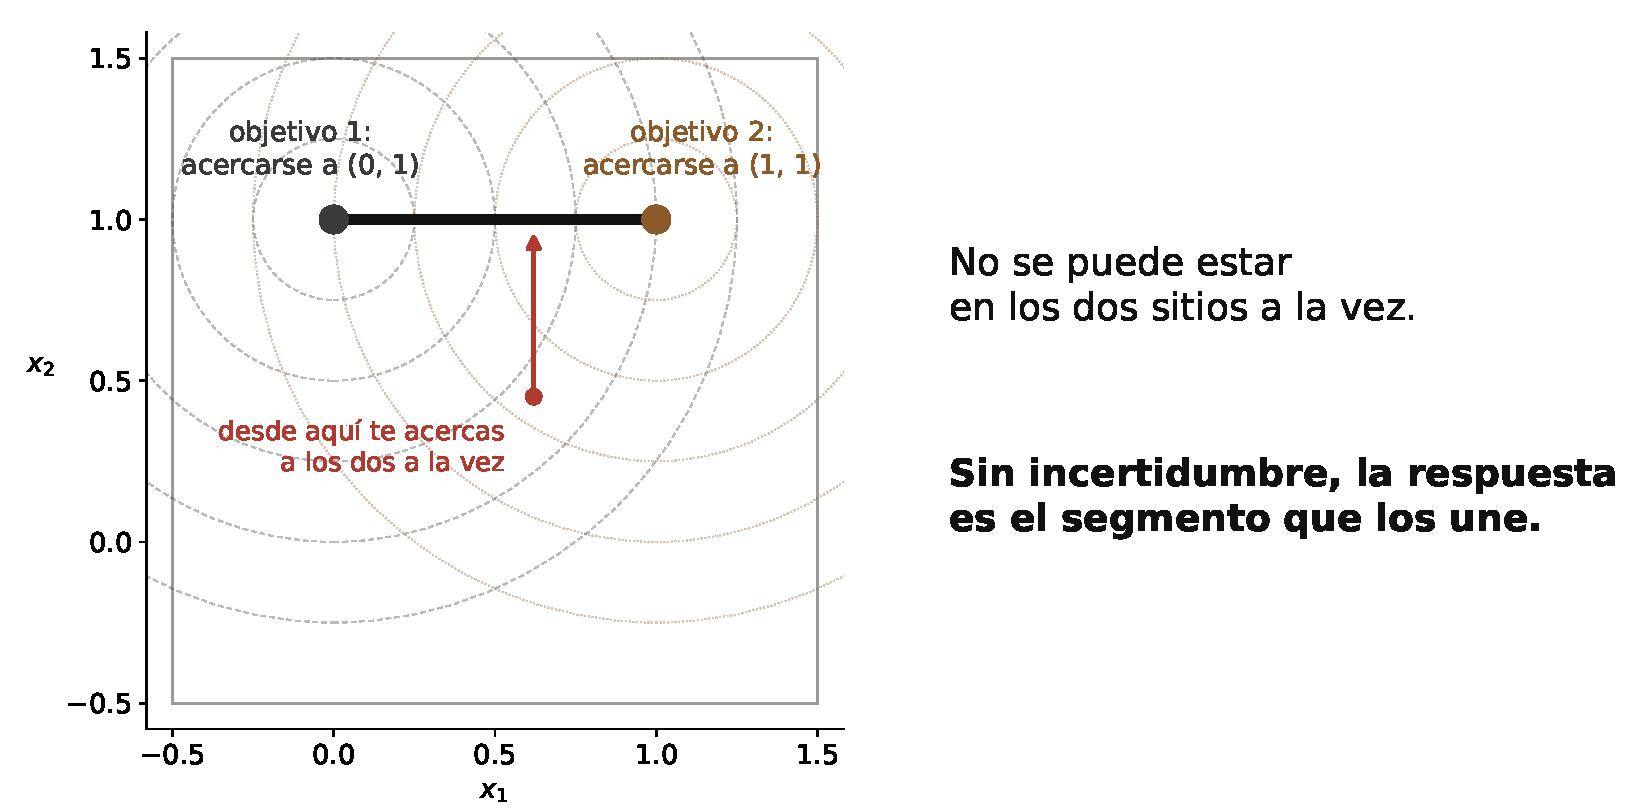
\includegraphics[width=0.99\textwidth,height=0.70\textheight,keepaspectratio]{p1_crisp.pdf}

  \vspace{-2mm}
  {\footnotesize Dos variables, un problema que se puede resolver a mano.}
  \NotaVI
\end{frame}

% ---------------------------------------------------------------- 7
\begin{frame}{p1, tres órdenes, tres respuestas distintas}
  \centering
  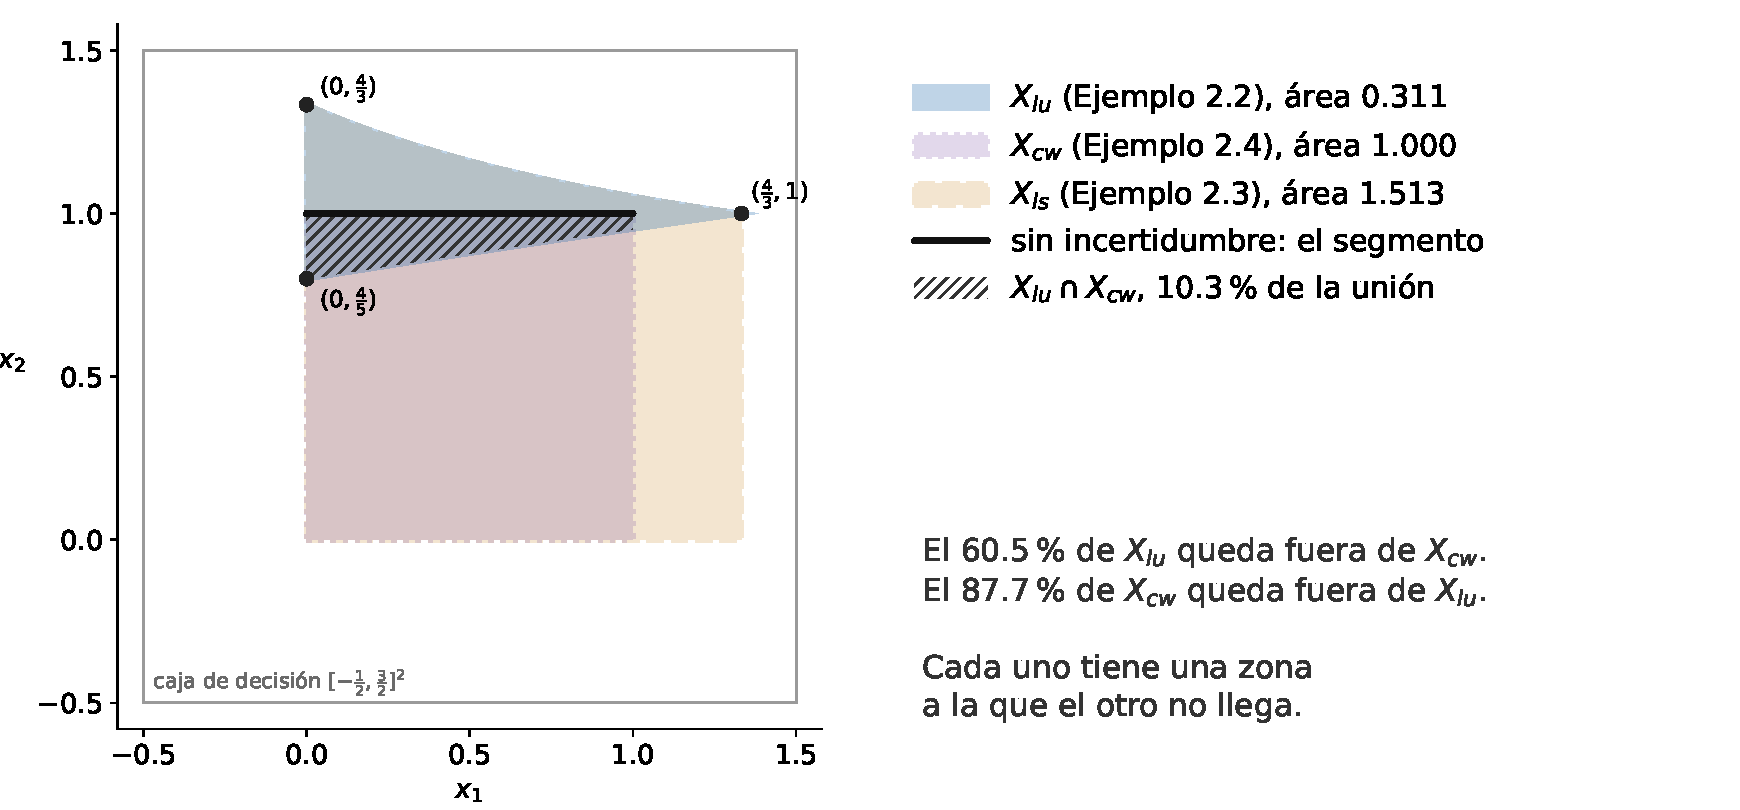
\includegraphics[width=0.98\textwidth,height=0.70\textheight,keepaspectratio]{p1_regiones.pdf}

  \vspace{-2mm}
  {\footnotesize De todo lo que podrían tener en común, sólo comparten el
  \textbf{\pUnionShare\,\%}. \cita{Y esto no lo ha calculado un ordenador: son las tres fórmulas dibujadas.}}
  \NotaVII
\end{frame}

% ---------------------------------------------------------------- 8
\begin{frame}{Y sé cuánto se equivoca lo que uso para medir}
  \centering
  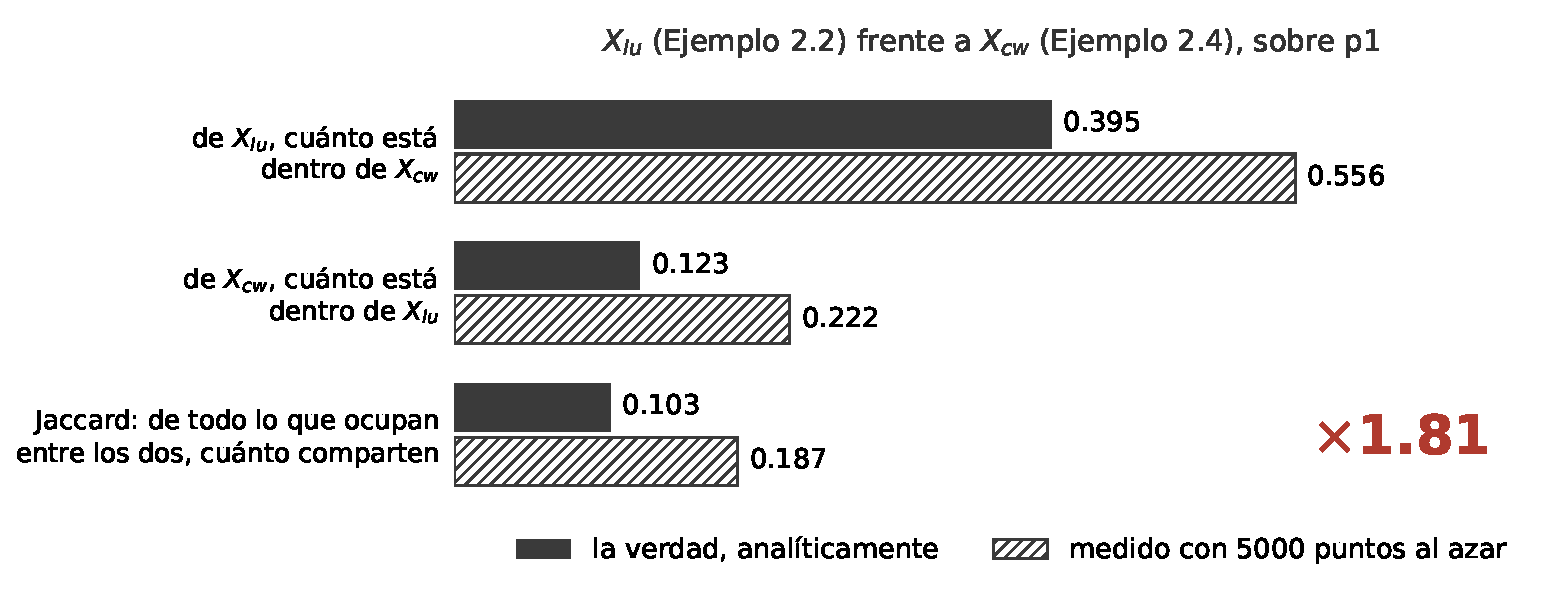
\includegraphics[width=0.97\textwidth,height=0.68\textheight,keepaspectratio]{instrumento.pdf}

  \vspace{-1mm}
  {\small Siempre en la misma dirección: al medir con puntos al azar, los dos
  órdenes salen \textbf{más parecidos de lo que son}.}
  \NotaVIII
\end{frame}

% ---------------------------------------------------------------- 9
\begin{frame}{Y ahora, p2, problemas de referencia del campo}
  \begin{columns}[T,onlytextwidth]
    \begin{column}{0.49\textwidth}
      \centering
      {\large\textbf{\ZdtName}} \quad \cita{\ZdtSize}\\[1mm]
      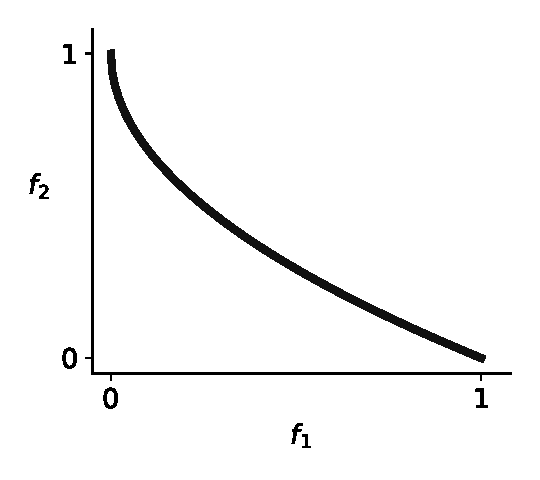
\includegraphics[height=0.33\textheight]{zdt1_frente.pdf}\\[-2mm]
      {\scriptsize $\ZdtF$\\[1mm] $\ZdtG$\\[0.5mm] \phantom{$\ZdtG$}}
    \end{column}
    \begin{column}{0.49\textwidth}
      \centering
      {\large\textbf{\DtlzName}} \quad \cita{\DtlzSize}\\[1mm]
      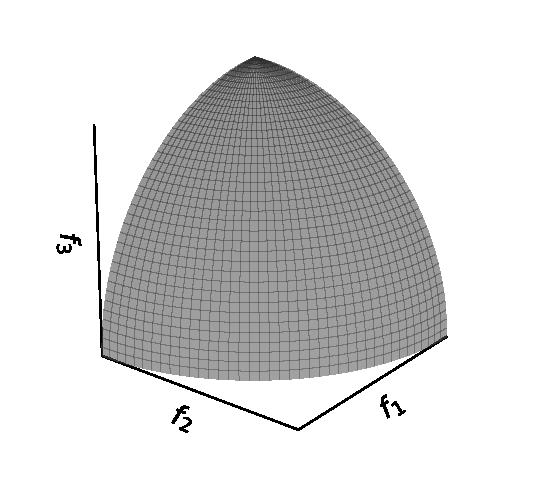
\includegraphics[height=0.33\textheight]{dtlz2_frente.pdf}\\[-2mm]
      {\scriptsize $\DtlzFone$\\[0.5mm] $\DtlzFtwo$\\[0.5mm] $\DtlzFthree$\\[1mm] $\DtlzG$}
    \end{column}
  \end{columns}
  \vspace{1mm}
  \begin{center}
    {\scriptsize Y a cada objetivo, su banda: \quad
    $\ZdtR$ \quad y \quad $\DtlzR$,\\[1mm]
    con $\marca{x_d}$ una variable que no está en el centro
    \cita{($\ZdtDrivers$ y $\DtlzDrivers$)} --- la regla de antes.}
  \end{center}
  \NotaIX
\end{frame}

% ---------------------------------------------------------------- 10
\begin{frame}{En p2: lo que te daba un orden, desaparece con el otro}
  \begin{columns}[c,onlytextwidth]
    \begin{column}{0.30\textwidth}
      \centering
      \begin{tikzpicture}[font=\tiny,scale=0.85,
          caja/.style={draw,rounded corners,minimum height=5mm,minimum width=18mm,align=center},
          filtro/.style={draw,rounded corners,minimum height=5mm,minimum width=13mm,align=center,thick},
          node distance=2.5mm and 4mm]
        \node[caja] (sample) {5000 puntos\\al azar};
        \node[caja,below=of sample] (eval) {una sola\\evaluación};
        \node[filtro,draw=phils,below=9mm of eval,xshift=4mm] (fls) {\pls};
        \node[filtro,draw=philu,below=of fls] (flu) {\plu};
        \node[filtro,draw=phicw,below=of flu] (fcw) {\pcw};
        \draw[-{Stealth}] (sample) -- (eval);
        % un carril a la izquierda, para que ninguna flecha cruce un cuadro
        \coordinate (lane) at ([xshift=-5mm]fls.west);
        \draw (eval.south) -- ++(0,-3mm) -| (lane);
        \draw (lane) -- (lane|-fcw.west);
        \draw[-{Stealth}] (lane|-fls.west) -- (fls.west);
        \draw[-{Stealth}] (lane|-flu.west) -- (flu.west);
        \draw[-{Stealth}] (lane|-fcw.west) -- (fcw.west);
        \node[below=3mm of fcw,align=center,gris,xshift=-2mm] {la misma lista, filtrada tres veces:\\lo único que cambia es el orden};
      \end{tikzpicture}
    \end{column}
    \begin{column}{0.68\textwidth}
      \centering
      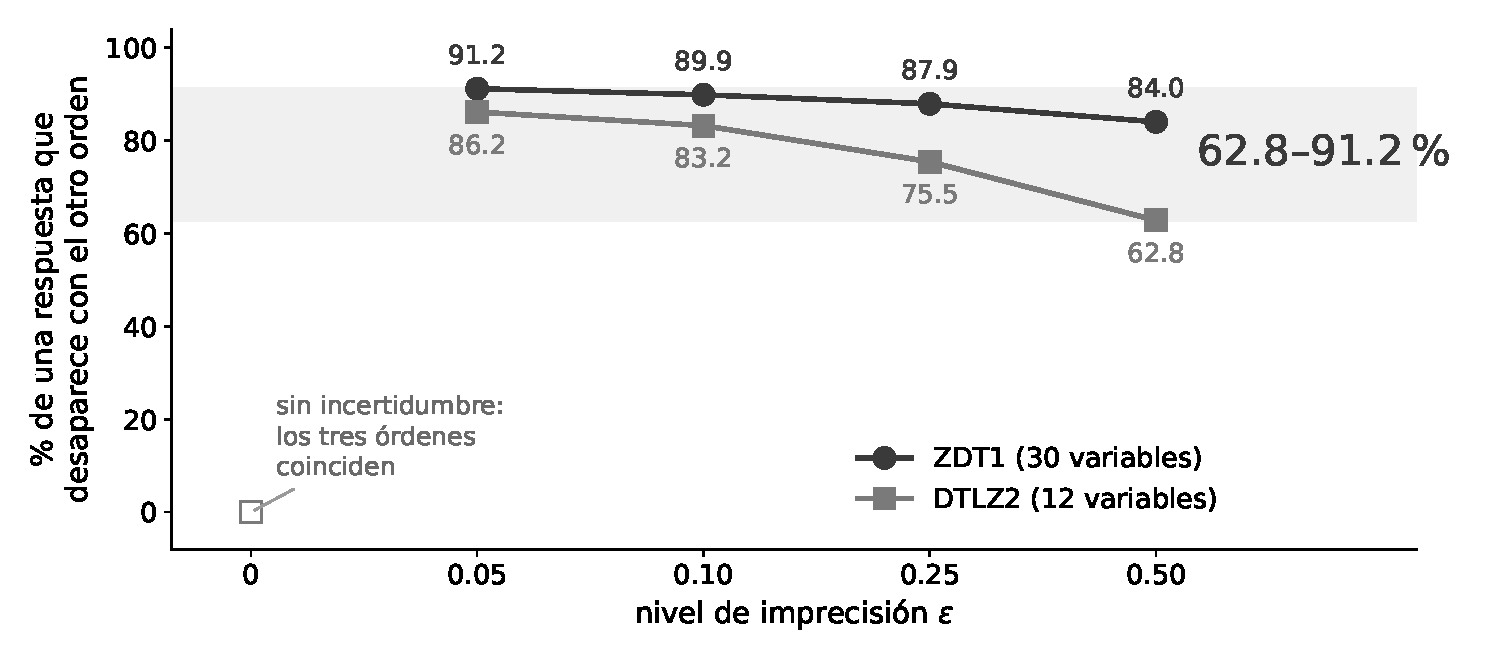
\includegraphics[width=0.98\textwidth,height=0.62\textheight,keepaspectratio]{benchmarks.pdf}
    \end{column}
  \end{columns}
  {\footnotesize Y como sé que mi medida dice que se parecen más de lo que se parecen, esto es un \textbf{mínimo}:
  \\ La diferencia real es mayor.}
  \NotaX
\end{frame}

% ---------------------------------------------------------------- 11
\begin{frame}{Y el tercero no lo he construido yo: está publicado}
  \centering
  \vspace{-2mm}
  {\footnotesize $\IBKone$,\quad $\IBKtwo$,\quad $x\in\IBKbox$}

  \vspace{-1mm}
  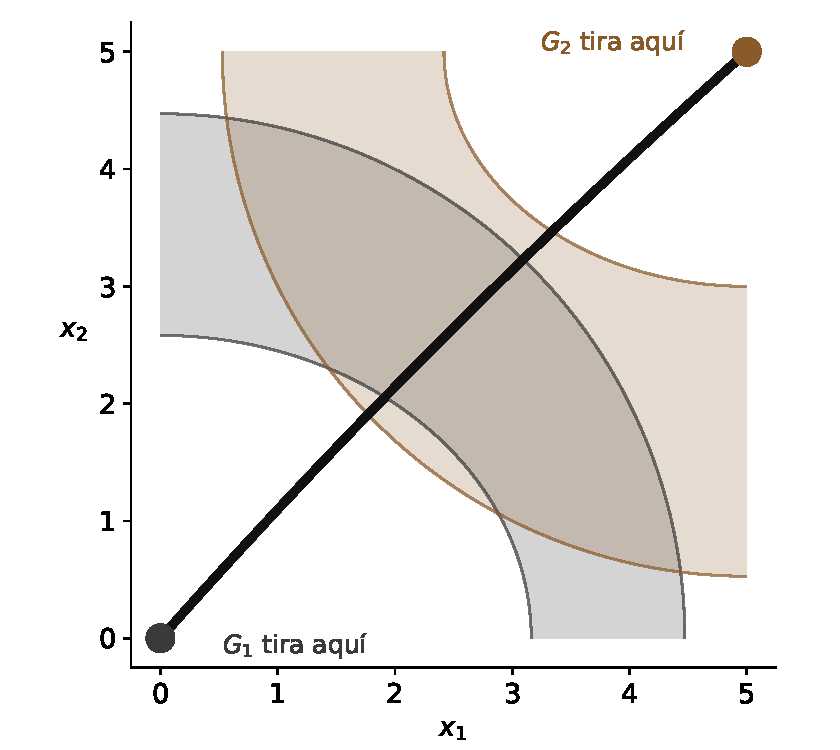
\includegraphics[height=0.69\textheight,keepaspectratio]{ibk1_crisp.pdf}

  \vspace{-1mm}
  {\footnotesize Cada objetivo vale un intervalo.}
  \NotaXI
\end{frame}

% ---------------------------------------------------------------- 12
\begin{frame}{Tres órdenes, tres respuestas: otra vez, y sin tocar el problema}
  \centering
  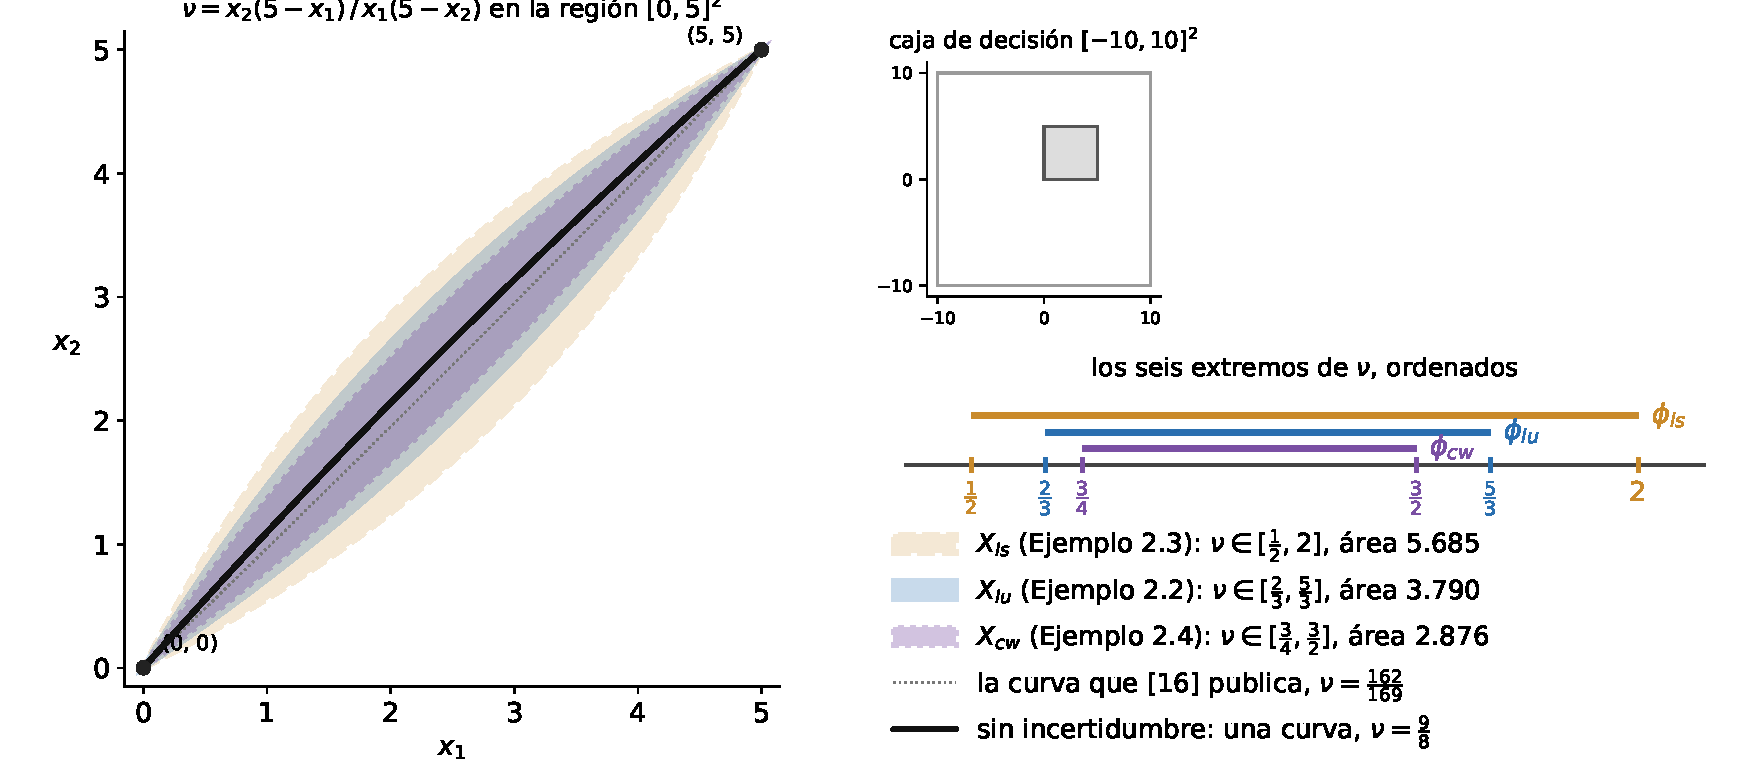
\includegraphics[width=0.98\textwidth,height=0.63\textheight,keepaspectratio]{ibk1_cunas.pdf}

  \vspace{-2mm}
  {\footnotesize Aquí las tres se meten una dentro de otra en vez de cruzarse: el
  \bMinInt--\bMaxInt\,\% de antes no vale aquí.\\ Lo que sí es
  exacto: el \textbf{\iLsOutsideCw\,\%} de la mayor queda fuera de la menor.}
  \NotaXII
\end{frame}

% ---------------------------------------------------------------- 13
\begin{frame}{Y de paso: el punto que publican como óptimo no lo es}
  \centering
  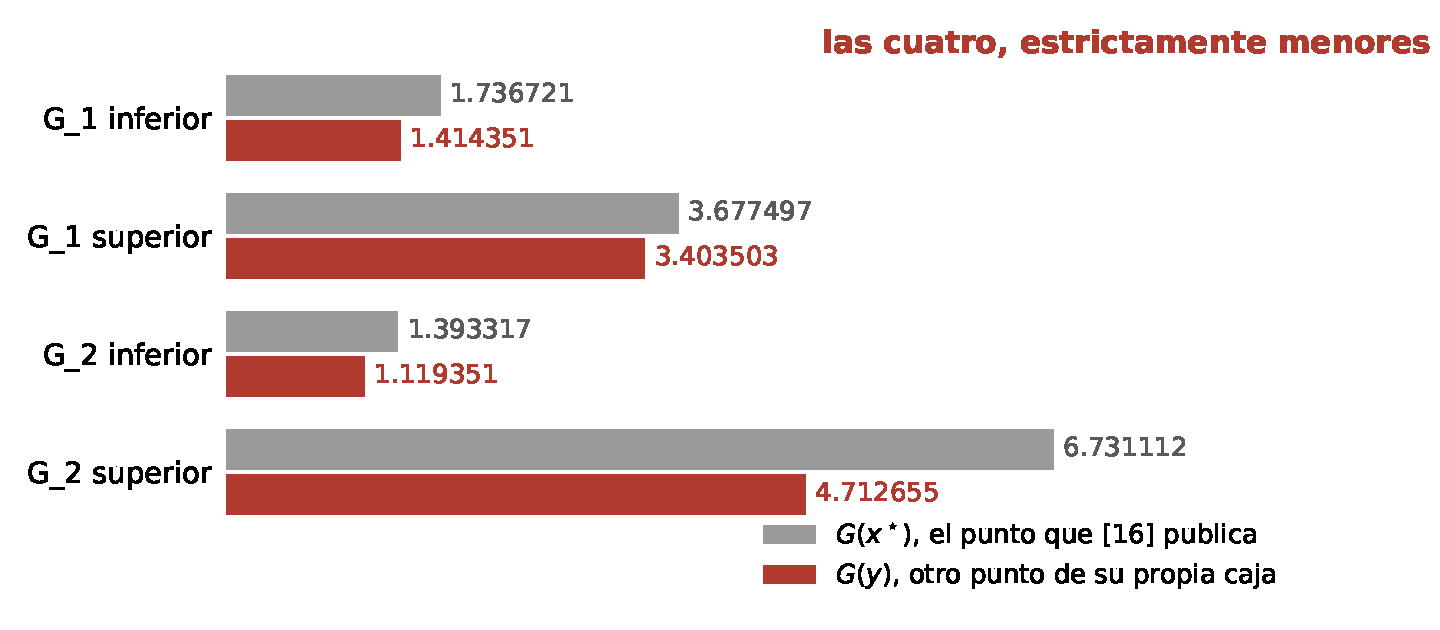
\includegraphics[width=0.88\textwidth,height=0.70\textheight,keepaspectratio]{contraejemplo.pdf}

  \vspace{-1mm}
  {\small Los de arriba son sus números; los de abajo salen con una calculadora
  en dos minutos.\\ \cita{Y los tres algoritmos lo encuentran.}}
  \NotaXIII
\end{frame}

% ---------------------------------------------------------------- cierre
\begin{frame}{Conclusiones}
  \vspace{4mm}
  \begin{center}
    \begin{minipage}{0.88\textwidth}
      {\large Elegir el orden no es un detalle de cómo montas el problema:\\
      \textbf{si no que condiciona la respuesta}.}
    \end{minipage}
  \end{center}
  \vspace{8mm}
  \begin{columns}[T,onlytextwidth]
    \begin{column}{0.32\textwidth}
      \centering
      {\LARGE\textbf{\pUnionShare\,\%}}\\[3mm]
      {\small es todo lo que dos órdenes\\ tienen en común}\\[2mm]
    \end{column}
    \begin{column}{0.32\textwidth}
      \centering
      {\LARGE\textbf{\bMinInt--\bMaxInt\,\%}}\\[3mm]
      {\small de tu respuesta desaparece\\ si te pasas al otro orden}\\[2mm]
    \end{column}
    \begin{column}{0.32\textwidth}
      \centering
      {\LARGE\textbf{\iLsOutsideCw\,\%}}\\[3mm]
      {\small de la respuesta mayor\\ se queda fuera de la menor}\\[2mm]
    \end{column}
  \end{columns}
  \vspace{7mm}
  \begin{center}
    \cita{Y siempre depende del problema: cada cifra viene de un problema concreto.}
  \end{center}
  \NotaXIV
\end{frame}

% ---------------------------------------------------------------- líneas futuras
\begin{frame}{Líneas futuras}
  \vspace{10mm}
  \begin{center}
    \begin{minipage}{0.82\textwidth}
      {\large
      \textbf{La curva de sensibilidad}: ir pasando poco a poco de un orden a
      otro, y ver cómo se mueve la respuesta.\\[8mm]
      \textbf{La aplicación a optimización de carteras}}
    \end{minipage}
  \end{center}
  \NotaXV
\end{frame}

\begin{frame}[plain]
  \vspace{10mm}
  \begin{center}
    {\Huge Gracias}\\[10mm]
  \end{center}
\end{frame}
\end{document}